\documentclass[12pt,a4paper]{article}

% Using Packages {{{
\usepackage[margin=2cm]{geometry}
\usepackage{fontspec}
\usepackage{graphicx}
\usepackage[table]{xcolor}
\usepackage{tabularx}
%\usepackage{enumitem,amssymb}
\usepackage{multicol}
\usepackage{listings}
\usepackage{titlesec}
\usepackage{tocloft}
\usepackage{titling}
\usepackage{hyperref}
%\usepackage{setspace}
\usepackage{fancyvrb}
\usepackage{fontawesome5}
\usepackage{tikz}
\usepackage[most]{tcolorbox}
\usepackage{fancyhdr}
\usepackage[normalem]{ulem}
\usepackage{longtable}
% }}}
% Preambles {{{
% Color Definition {{{
\definecolor{backcolour}{rgb}{0.95,0.95,0.95}
\definecolor{keywordsColor}{rgb}{0.000000, 0.000000, 0.635294}
\definecolor{ndkeywordColor}{rgb}{0.558215, 0.000000, 0.135316}
\definecolor{stringColor}{rgb}{0.000000, 0.558215, 0.135316}
\definecolor{emphColor}{rgb}{0.000000, 0.135316, 0.558215}
%% some commented ones {{{
%\definecolor{commentsColor}{rgb}{0.497495, 0.497587, 0.497464}
%\definecolor{codegreen}{rgb}{0,0.6,0}
%\definecolor{mygray}{gray}{0.5}
%\definecolor{codepurple}{rgb}{0.58,0,0.82}
%\definecolor{armygreen}{rgb}{0.29, 0.33, 0.13}
%\definecolor{keywordsColor}{rgb}{0.000000, 0.000000, 0.635294}
%\definecolor{stringColor}{rgb}{0.558215, 0.000000, 0.135316}
%\definecolor{alizarin}{rgb}{0.82, 0.1, 0.26}
%\definecolor{frenchbeige}{rgb}{0.65, 0.48, 0.36}
%\definecolor{beaver}{rgb}{0.62, 0.51, 0.44}
%%
%%%\definecolor{bostonuniversityred}{rgb}{0.8, 0.0, 0.0}
%%%\definecolor{lavenderpurple}{rgb}{0.59, 0.48, 0.71}
%%%\definecolor{lavenderfloral}{rgb}{0.71, 0.49, 0.86}
%%%\definecolor{goldmetallic}{rgb}{0.83, 0.69, 0.22}
%%
%%%\definecolor{onyx}{rgb}{0.66, 0.66, 0.66}
%%%\definecolor{grullo}{rgb}{0.66, 0.6, 0.53}
%% }}}
% }}}
% Font Families {{{
%% Ubuntu {{{
%\newfontfamily\Ubfam{UbuntuMono}[
%Path				=	/home/hos/.fonts/ubuntu/,
%Extension			=	.ttf,
%UprightFont			=	*-R,
%BoldFont			=	*-B,
%ItalicFont			=	*-RI,
%BoldItalicFont		=	*-BI,
%%SmallCapsFont		=	*-C,
%%SlantedFont		=	*-Th,
%%BoldSlantedFont	=	*-,
%]
%% }}}
% Modern Computer {{{
\newfontfamily\Cmu{cmun}[
Path				=	/home/hos/.fonts/cmu/Code/,
Extension			=	.ttf,
UprightFont			=	*tt,
BoldFont			=	*tb,
ItalicFont			=	*it,
BoldItalicFont		=	*tx,
%SmallCapsFont		=	*tt,
%SlantedFont		=	*-Th,
%BoldSlantedFont	=	*-,
]
% }}}
%% Neuton {{{
%\newfontfamily\Neu{Neuton}[
%Path			=   /home/hos/.fonts/neuton/,
%Extension	   =   .ttf,
%UprightFont	 =   *-Regular,
%BoldFont		=   *-Bold,
%ItalicFont	  =   *-Italic,
%%BoldItalicFont  =   *-BoldItalic,
%SmallCapsFont   =   *Cursive-Regular,
%%SlantedFont	 =   *-Th,
%%BoldSlantedFont =   *-,
%]
%% }}}
% Fira-script {{{
\newfontfamily\FiraCiS{FiraCodeiScript}[
Path				=	/home/hos/.fonts/FiraCodeiScript/,
Extension			=	.ttf,
UprightFont			=	*-Regular,
BoldFont			=	*-Bold,
ItalicFont			=	*-Italic,
%BoldItalicFont		=	*-BoldItalic,
%SmallCapsFont		=	*Cursive-Regular,
%SlantedFont		=	*-Th,
%BoldSlantedFont	=	*-,
]
% }}}
% Fira-script {{{
\newfontfamily\CodeNewR{Code New Roman}[
Path				=	/home/hos/.fonts/code-new/,
Extension			=	.otf,
UprightFont			=	*,
BoldFont			=	* b,
ItalicFont			=	* i,
%BoldItalicFont		=	*-BoldItalic,
%SmallCapsFont		=	*Cursive-Regular,
%SlantedFont		=	*-Th,
%BoldSlantedFont	=	*-,
]
% }}}
%\setmainfont{Liberation Serif}
%\setmainfont{FreeSerif}
%\setmainfont{Spectral}
%\setmainfont{IBM Plex Serif}
%\setmainfont{Avrile Serif}
%
%\setsansfont{Liberation Sans}
%\setsansfont{Ubuntu}
\setmainfont{Libertinus Serif}
\setsansfont{Ubuntu}
\setmonofont{Fira Mono}
%
%\setmonofont{UbuntuMono-Regular}
% }}}
%% Global Code:Block Formatting {{{
%\lstset{frame=tb,
%  language=c,
%  showstringspaces=false,
%  columns=flexible,
%  numbers=left,
%   xleftmargin=.03\textwidth,
%  xrightmargin=.03\textwidth,
%%
%  basicstyle={\ttfamily\footnotesize},
%  commentstyle={\itshape},
%  emphstyle={\underline},
%  stringstyle={\bfseries\normalsize\Cmu},
%  numberstyle={\ttfamily\scriptsize\color{black!50!white}},
%%
%  rulecolor=\color{black!50!white},
%%
%%  keywordstyle={\color{codepurple}},
%%  commentstyle={\color{frenchbeige}},
%%  stringstyle={\color{alizarin}},
%%  keywordstyle={\color{codepurple}},
%%  ndkeywordstyle={\ttfamily\color{keywordsColor}},
%%  emph={ls},
%%  emphstyle={\color{red}},
%%  backgroundcolor=\color{white!96!black},
%%  ndkeywordstyle={\underline},
%  morekeywords={True, False,},
%  emph={unsigned, int, char, void, float, bool, FILE},
%%  emphstyle={\color{red}},
%  breaklines=true,
%  breakatwhitespace=false,
%  numbersep=3mm,
%  frame=leftline,
%%  frame=left top right bottom,
%%  caption=\code{e.g.},
%%  frame=shadowbox,
%%  frame=none,
%%
%  aboveskip=5mm,
%  belowskip=2mm,
%  captionpos=t,
%  tabsize=8
%}
%% end code block formatting }}}
% code block formatting {{{
%% Python {{{
%\lstdefinelanguage{Python}{
	%sensitive=true,
	%comment=[l]{\#},
	%string=[b]{"},
	%string=[b]{'},
	%keywords={print, input, range, type, return},
	%ndkeywords={in, if, else, for, while, def},
	%emph={and, or, not, True, False,},
	%%literate=%
	%%*{0}{{\color{red!70!black}0}}1
		%%{1}{{\color{red!70!black}1}}1
		%%{2}{{\color{red!70!black}2}}1
		%%{3}{{\color{red!70!black}3}}1
		%%{4}{{\color{red!70!black}4}}1
		%%{5}{{\color{red!70!black}5}}1
		%%{6}{{\color{red!70!black}6}}1
		%%{7}{{\color{red!70!black}7}}1
		%%{8}{{\color{red!70!black}8}}1
		%%{9}{{\color{red!70!black}9}}1
%}
%% }}}
% JavaScript {{{
\lstdefinelanguage{JavaScript} {
	keywords={break, case, catch, continue, debugger,
		default, delete, do, else, false, finally, for,
		function, if, in, instanceof, new, null, return,
		switch, this, throw, true, try, typeof, var, void,
		while, with
	},
	morecomment=[l]{//},
	morecomment=[s]{/*}{*/},
	morestring=[b]',
	morestring=[b]",
	ndkeywords={class, export, boolean, throw, implements, import, this, script},
	emph={language, type},
	sensitive=true
}
% }}}
% Global {{{
\lstset{
	language=python,
	showstringspaces=false,
	columns=flexible,
	basicstyle={\ttfamily\small},
	numbers=left,
	xleftmargin=.03\textwidth,
	xrightmargin=.03\textwidth,
	emph={ True, False, None, __iter__, __next__, __init__,
		random, platform, datetime, math, json, re, os, statistics,
		requests, 
	},
	morendkeywords={lower, upper, strip, replace, split,
		capitalize, casefold, center, count, encode,
		endswith, expandtabs, find, format_map,
		index, isalnum, isalpha, isdecimal, isdigit,
		islower, isnumeric, isprintable, isspace, istitle,
		isidentifier, isupper, join, ljust,  lstrip,
		maketrans, partition, rfind, rindex, rjust,
		rpartition, rsplit, rstrip,  splitlines, startswith,
		swapcase, title, translate,  zfill, append, insert,
		extend, clear, pop, remove, sort, copy, reverse,
		update, add, discard, union, intersection_update,
		intersection, difference, difference_update,
		symmetric_difference, symmetric_difference_update,
		isdisjoint, issubset, issuperset, get, keys, values,
		items, fromkeys, popitem, setdefault, self, now,
		sqrt, ceil, floor, loads, dumps, search, findall,
		sub, system, strftime, span, string, group, write, close,
		Exception, TypeError, isqrt, rmdir, path, exists, 
		acos, acosh, asin, asinh, atan, atan2, atanh, comb, copysign, cos, cosh,
		degrees, dist, erf, erfc, exp, expm1, fabs, factorial, fmod, frexp, fsum,
		gamma, gcd, hypot, isclose, isfinite, isinf, isnan, ldexp, lgamma, log, log10,
		log1p, log2, perm, prod, radians, remainder, sin, sinh, tan, tanh, trunc, 
		seed, getstate, setstate, getrandbits, randrange, randint, choice, choices,
		shuffle, sample, random, uniform, triangular, betavariate, expovariate,
		gammavariate, gauss, lognormvariate, normalvariate, vonmisesvariate,
		paretovariate, weibullvariate, read, text, 
		delete, get, head, patch, post, put, request,
		harmonic_mean, mean, median, median_grouped, median_high,
		median_low, mode, pstdev, stdev, pvariance, variance
	},
	morekeywords={as, input},
%
	%keywordstyle={\bfseries},
	%emphstyle={\color{white!25!black}\itshape},
	%ndkeywordstyle={\bfseries\CodeNewR\color{white!20!black}},
	%stringstyle={\CodeNewR\color{white!30!black}},
%
	emphstyle={\color{red!50!blue}\FiraCiS},
	ndkeywordstyle={\CodeNewR\color{ndkeywordColor}},
	stringstyle={\color{stringColor}},
	keywordstyle={\color{keywordsColor}},
%
	commentstyle={\CodeNewR\color{white!50!black}},
	numberstyle={\ttfamily\scriptsize\color{white!60!black}},
	rulecolor=\color{black!50!white},
	breaklines=true,
	breakatwhitespace=false,
	numbersep=3mm,
	%frame=none,
	frame=leftline,
	%frame=left top right bottom,
	aboveskip=2mm,
	belowskip=2mm,
	escapechar=\`,
	captionpos=t,
	tabsize=4
}
% }}}
% }}}
% Macros {{{
% centered text box {{{
\newcommand{\wspace}[1]{%
	\color{white}\colorbox{white}{\texttt{#1}}%
}
% }}}
% in-line code {{{
\newcommand{\code}[1]{%
	\colorbox{backcolour}{\lstinline{#1}}%
}
% }}}
% in-line code no-bg {{{
\newcommand{\lcode}[1]{%
	\lstinline{#1}%
}
% }}}
% Figures {{{
\newcommand{\picin}[3]{%
	\begin{figure}[h]
	\begin{center}
		\includegraphics[width=#3\textwidth]{#1}
	\end{center}
		\caption{#2}
	\end{figure}
}
% }}}
% table two column {{{
\newcommand{\tcol}[2]{%
	\quad #1 & #2 \\
}
% }}}
% table three column {{{
\newcommand{\trcol}[3]{%
	#1 \quad  & #2 & #3 \\
}
% }}}
% items {{{
\newcommand{\titem}[2]{%
%$\circ$
\item #1: #2
}
% }}}
% }}}

% vercode {{{
\DefineVerbatimEnvironment{vercode}{Verbatim}%
	{fontsize=\small,
		fontfamily=tt,
		gobble=0,
		%frame=leftline,
		%frame=single,
		%frame=none,
		%frame=topline,
		frame=lines,
		framerule=0mm,
		framesep=2mm,
		baselinestretch=1.1,
		labelposition=topline,
		%numbers=left,
		samepage=true,
		%commandchars=+\[\]
}
% }}}
% alert box env {{{
\newtcolorbox{abox}{
	title={\centering\color{red!70!black}{\textsf{Error}\hspace{2mm}\faExclamationTriangle}},
	boxrule=1pt,
	arc = 0.05mm,
	sharp corners = all,
	enlarge top by=3mm,
	minipage boxed title*=-15cm,
	beamer,
	enhanced,
	center,
	%attach boxed title to top center={yshift=-2.5mm},
	attach boxed title to top right={yshift=-2mm, xshift=-1cm},
	colback  = red!05!white,
	colframe = red!70!black,
	colbacktitle = white,
}
% }}}
% test box env {{{
\newtcolorbox{tbox}{
	title={\centering\color{blue!70!black}{\textsf{Test}\hspace{2mm}\faClipboard[regular]}},
	boxrule=1pt,
	arc = 0.05mm,
	sharp corners = all,
	enlarge top by=3mm,
	minipage boxed title*=-15cm,
	beamer,
	enhanced,
	center,
	%attach boxed title to top center={yshift=-2.5mm},
	attach boxed title to top right={yshift=-2mm, xshift=-1cm},
	colback  = blue!05!white,
	colframe = blue!70!black,
	colbacktitle = white,
}
% }}}
% note box env {{{
\newtcolorbox{nbox}{
	title={\centering\color{green!50!black}{\textsf{Note}\hspace{2mm}\faExclamationCircle}},
	boxrule=1pt,
	arc = 0.05mm,
	%sharp corners = all,
	enlarge top by=3mm,
	minipage boxed title*=-15cm,
	beamer,
	enhanced,
	center,
	%attach boxed title to top center={yshift=-2.5mm},
	attach boxed title to top right={yshift=-2mm, xshift=-1cm},
	colback  = green!07!white,
	colframe = green!50!black,
	colbacktitle = white,
}
% }}}
% exmaple box env {{{
\newtcolorbox{ebox}{
	title={\centering \color{black}{\textsf{Example} }},
	boxrule=1pt,
	arc = 0.5mm,
	%sharp corners = downhill,
	enlarge top by=3mm,
	minipage boxed title*=-15cm,
	beamer,
	enhanced,
	center,
	%attach boxed title to top center={yshift=-2.5mm},
	attach boxed title to top left={yshift=-2mm, xshift=1cm},
	colback  = black!03!white,
	colframe = black!90!white,
	colbacktitle = white,
}
% }}}
% no box env {{{
\newtcolorbox{bbox}{
	%title={\centering \color{black}{\textsf{Example} }},
	boxrule=1pt,
	arc = 0.5mm,
	%sharp corners = downhill,
	enlarge top by=3mm,
	minipage boxed title*=-15cm,
	beamer,
	enhanced,
	center,
	%attach boxed title to top center={yshift=-2.5mm},
	attach boxed title to top left={yshift=-2mm, xshift=1cm},
	colback  = black!03!white,
	colframe = black!90!white,
	colbacktitle = white,
}
% }}}
% tcb env {{{
\newtcolorbox{tcb}[1][]{
	title={\centering \color{black}{#1}},
	boxrule=1pt,
	arc = 0.5mm,
	%sharp corners = downhill,
	enlarge top by=3mm,
	minipage boxed title*=-15cm,
	beamer,
	enhanced,
	center,
	attach boxed title to top center={yshift=-2.5mm},
	%attach boxed title to top right={yshift=-2.5mm, xshift=-1cm},
	colback  = black!03!white,
	colframe = black!90!white,
	colbacktitle = white,
}
% }}}

% Formatting {{{
%% part {{{
%\titleformat{\part}{\huge\bfseries}{}{1em}{}
%\titleformat{\part}[display]
	%{\filcenter}
	%{}
	%{-5mm}
	%{\LARGE}
	%[\vspace{1cm}]
%
%\titlecontents{part}[0pt]
	%{\bfseries\protect\addvspace{15pt}\titlerule[1pt]\addvspace{1.2ex}}
	%{}
	%{\color{blue!60!black}\partname~}%numbered, unnumbered
	%{\hfill\contentspage}
	%[\addvspace{0.7ex}{\titlerule[1pt]}\addvspace{1.5ex}]
%% }}}
% Sections {{{
\titleformat{\section} {\Large\bfseries\sffamily}
{\thesection\quad}{0em}{}[{\titlerule[0pt]}]
\titlespacing{\section}{0pt}{7mm}{5mm}

\titleformat{\subsection} {\large\bfseries\sffamily}
{\thesubsection\quad}{0em}{}[{\titlerule[0pt]}]
\titlespacing{\subsection}{0pt}{7mm}{3mm}

\titleformat{\subsubsection} {\bfseries\sffamily}
{\thesubsubsection\quad}{0em}{}
\titlespacing{\subsubsection}{0pt}{7mm}{3mm}

% }}}
% toc {{{
\cftsetindents{subsection}{1em}{3em}
% }}}
\setlength{\parindent}{0mm}
\setlength{\headheight}{13pt}
%\onehalfspacing
\linespread{1.2}
% }}}
% Links color {{{
\hypersetup{
	colorlinks=true,
	linkcolor={blue!60!black},
	urlcolor={blue!60!green},
	citecolor={red!75!yellow},
	pdftitle={Python},
}
% }}}

%% Persian font {{{
%\usepackage{xepersian}
%\settextfont{Yas}
%\ExplSyntaxOn \cs_set_eq:NN \etex_iffontchar:D \tex_iffontchar:D \ExplSyntaxOff
%
%\defpersianfont\nast{IranNastaliq}
%\defpersianfont\titre{XB Titre}
%\defpersianfont\khali{XB Kayhan Sayeh}
%\defpersianfont\yekan{XM Yekan}
%% }}}

% Title {{{
\title{\textbf{Python Programming} \\ \vspace{1cm} {\Large Basics}}
\author{PJ}
\date{}
% }}}
% }}}

\begin{document}
%% start alternating shades from 3rd row
\rowcolors{2}{white!96!black}{white}
\setcounter{tocdepth}{2}
% Body {{{

% beginning {{{
\pagestyle{fancy}
\maketitle
%\vspace{1cm}
\vfill\newpage
\pagestyle{fancy}
\pagenumbering{roman}
\renewcommand{\headrulewidth}{0pt}
\addtolength{\topmargin}{-1.49998pt}
\setlength{\headheight}{14.49998pt}
\renewcommand{\sectionmark}[1]{%
\markboth{\thesection\quad #1}{}}
\fancyhead[R]{}
\fancyhead[C]{}
\fancyhead[L]{}
\fancyfoot{}
\fancyfoot[R]{(\thepage)}
\fancyfoot[C]{}
\fancyfoot[L]{}
\tableofcontents
\vfill\newpage
%\fancyhf{}
%\fancyhead[L]{\rightmark}
%\fancyhead[R]{\thepage}
\renewcommand{\headrulewidth}{0.3pt}
\addtolength{\topmargin}{-1.49998pt}
\setlength{\headheight}{14.49998pt}
\renewcommand{\sectionmark}[1]{%
\markboth{\thesection\quad #1}{}}
\fancyhead[R]{\rightmark}
\fancyhead[C]{}
\fancyhead[L]{\leftmark}
\fancyfoot{}
\fancyfoot[R]{(\thepage)}
\fancyfoot[C]{}
\fancyfoot[L]{}

%\pagestyle{scrheadings}
%\clearpairofpagestyles
%%\ohead{\rightmark}
%\lohead{\thesection}
%\rehead{\thesubsection}
%%\cfoot[\pagemark]{\pagemark}
% }}}
\pagenumbering{arabic}
% }}}
% finished {{{
% intro {{{
\section{Python Introduction}
\subsection{What is Python?}
Python is a popular programming language. It was created by {\itshape Guido van Rossum}, and released in 1991.

It is used for:

\begin{itemize}
	\item web development (server-side)
	\item software development
	\item mathematics
	\item system scripting
\end{itemize}

\subsection{What can Python do?}

\begin{itemize}
	\item Python can be used on a server to create web applications.
	\item Python can be used alongside software to create workflows.
	\item Python can connect to database systems. It can also read and modify files.
	\item Python can be used to handle big data and perform complex mathematics.
	\item Python can be used for rapid prototyping, or for production-ready software development
\end{itemize}

\subsection{Why Python?}

\begin{itemize}
	\item Python works on different platforms (Windows, Mac, Linux, Raspberry Pi, etc).
	\item Python has a simple syntax similar to the English language.
	\item Python has syntax that allows developers to write programs with fewer lines than some other programming languages.
	\item Python runs on an interpreter system, meaning that code can be executed as soon as it is written. This means that prototyping can be very quick.
	\item Python can be treated in a procedural way, an object-oriented way or a functional way.
\end{itemize}

\subsection{Good to know}

\begin{itemize}
	\item The most recent major version of Python is Python 3, which we shall be using in this tutorial. However, Python 2, although not being updated with anything other than security updates, is still quite popular.
	\item In this tutorial Python will be written in a text editor. It is possible to write Python in an Integrated Development Environment, such as Thonny, Pycharm, Netbeans or Eclipse which are particularly useful when managing larger collections of Python files.
\end{itemize}

\subsection{Python Syntax compared to other programming languages}

\begin{itemize}
	\item Python was designed for readability, and has some similarities to the English language with influence from mathematics.
	\item Python uses new lines to complete a command, as opposed to other programming languages which often use semicolons or parentheses.
	\item Python relies on indentation, using whitespace, to define scope; such as the scope of loops, functions and classes. Other programming languages often use curly-brackets for this purpose.
\end{itemize}

\begin{tcb}[Python]
\begin{lstlisting}[numbers=none,xrightmargin=0mm,xleftmargin=0mm,frame=none]
print("Hello World!")
\end{lstlisting}
\end{tcb}

\begin{tcb}[C]
\begin{lstlisting}[language=c,numbers=none,xrightmargin=0mm,xleftmargin=0mm,frame=none]
#include <stdio.h>
int main(void) {
      printf("Hello World!\n");
      return 0;
}
\end{lstlisting}
\end{tcb}

\begin{tcb}[Java]
%\filcenter
\begin{lstlisting}[language=Java,numbers=none,xrightmargin=0mm,xleftmargin=0mm,frame=none]
class HelloWorld {
      public static void main(String[] args) {
          System.out.println("Hello, World!");
      }
}
\end{lstlisting}
\end{tcb}
% }}}
\vfill\newpage
% getting started {{{
\section{Getting Started}
% Installation {{{
\subsection{Installations}
Many PCs and Macs will have python already installed.

To check if you have python installed on a Windows PC, search in the start bar
for Python or run the following on the Command Line (cmd.exe):

\begin{vercode}
C:\Users\Your Name> python --version
\end{vercode}

To check if you have python installed on a Linux or Mac, then on linux open the
command line or on Mac open the Terminal and type:

\begin{vercode}
$ python --version
\end{vercode}

% Install Python {{{
% Windows {{{
\subsubsection{Install Python on Windows}

If you find that you do not have Python installed on your computer, then you
can download it for free from the following website:
\underline{\href{https://www.python.org/}{python.org}}.

\begin{center}
	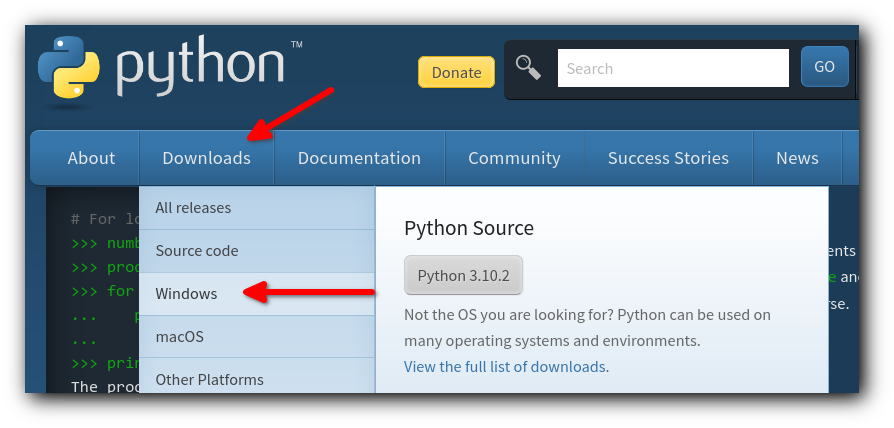
\includegraphics[width=.9\textwidth]{shots/installation/python-page.png}
\end{center}

Download and install \textsf{Latest Python 3 Release - Python 3.X}

\begin{center}
	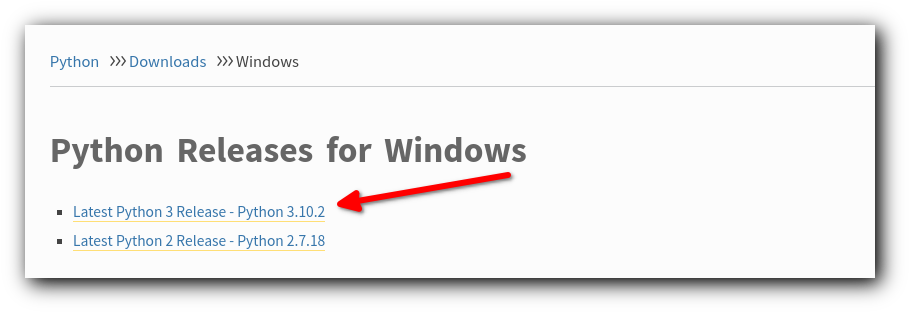
\includegraphics[width=.9\textwidth]{shots/installation/python-version.png}
\end{center}

I'd prefer to go with \textsf{Recommended} versions

\begin{center}
	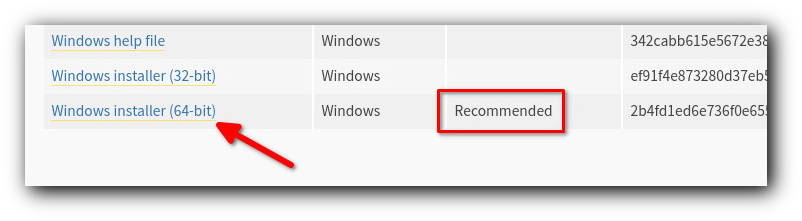
\includegraphics[width=.9\textwidth]{shots/installation/python-download.png}
\end{center}
% }}}
% Linux {{{
\subsubsection{Install Python on Linux}
The best way to install Python on Linux, is installing it from
our distribution's \texttt{Package Manager}.

\begin{itemize}
\item {Ubuntu/Mint/Debian:}
	\code{\$ sudo apt install python3}

\item {Arch/Manajaro:}
	\code{\$ sudo pacman -Sy python}

\item {Redhat/Fedora:}
	\code{\$ sudo dnf install python}

\item {OpenSUSE:}
	\code{\$ sudo zypper install python}
\end{itemize}
% }}}
% }}}
% Install Editor {{{
\subsubsection{Install Text-editor/IDE}
To writing Python programs, we can use any text editor or IDE
which we are comfortable with.
For example we are going to install \textsf{VSCodium} here
and set it up for Python development.

First of all, we need to go to its website and download the software
from its webstie:
\underline{\href{https://vscodium.com}{vscodium.com}}.

\begin{center}
	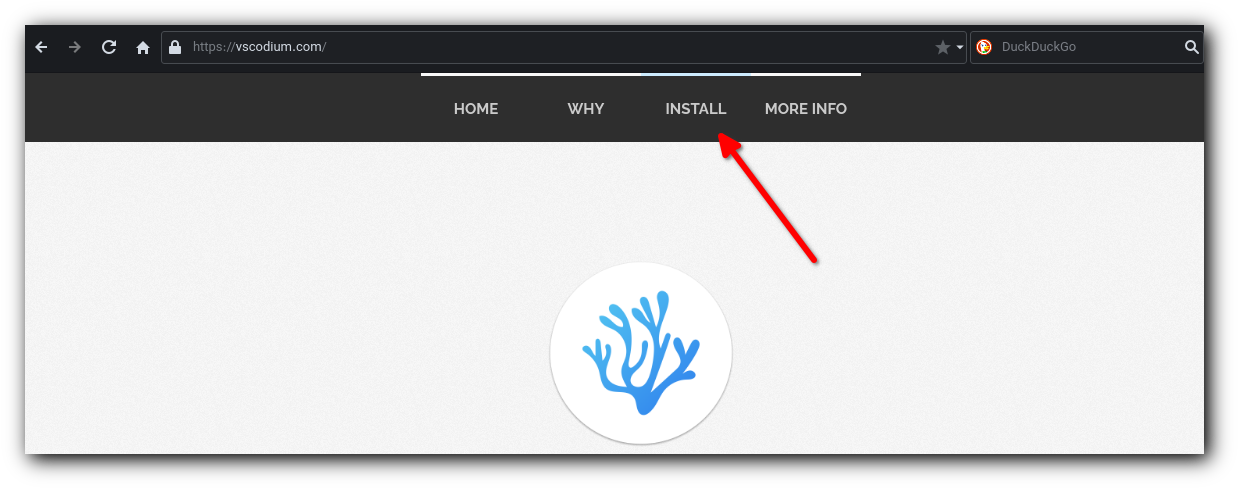
\includegraphics[width=.9\textwidth]{shots/installation/vscodium-page.png}
\end{center}

Go download and install the latest version of VSCodium.

\begin{center}
	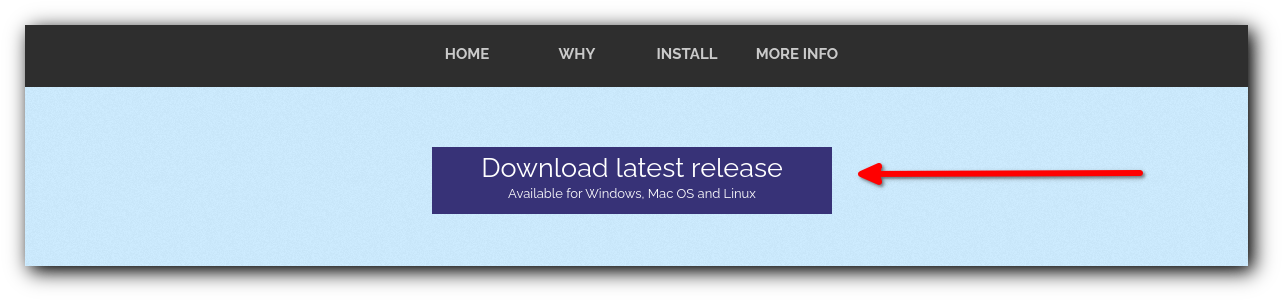
\includegraphics[width=.9\textwidth]{shots/installation/vscodium-download.png}
\end{center}

\begin{center}
	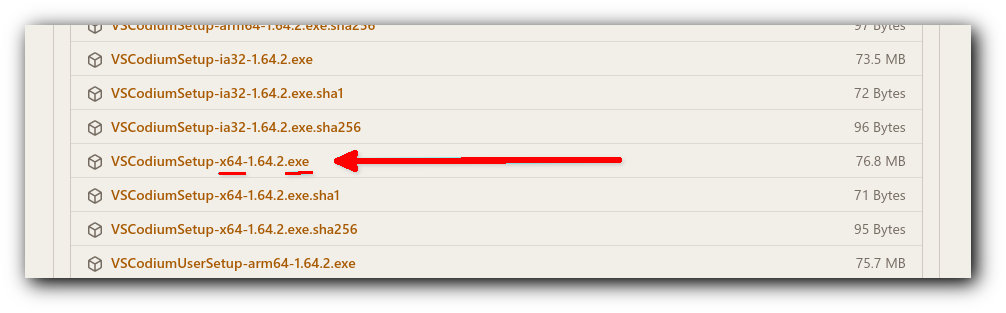
\includegraphics[width=.9\textwidth]{shots/installation/vscodium-version.png}
\end{center}
% }}}
% setup vscodium {{{
\subsubsection{Setup VSCodium}
After installing VSCodium, we need to install python extension on it
to run and debug our python programs:

\begin{center}
	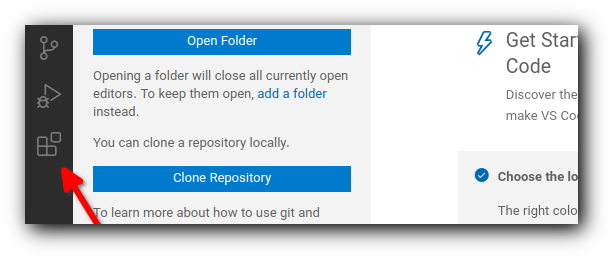
\includegraphics[width=.9\textwidth]{shots/installation/vscodium-first-open.png}

	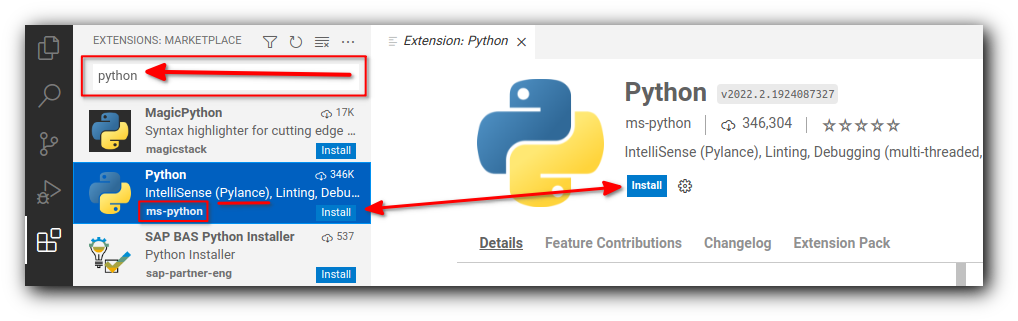
\includegraphics[width=.9\textwidth]{shots/installation/vscodium-extention.png}

	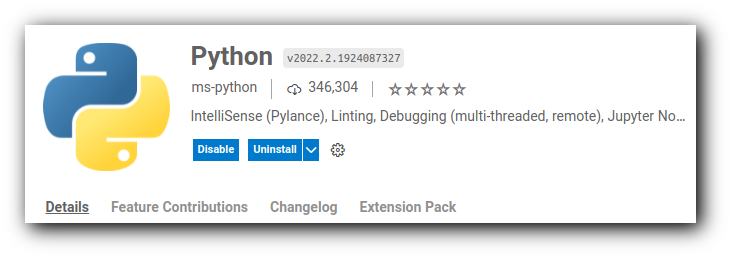
\includegraphics[width=.9\textwidth]{shots/installation/vscodium-extention-installed.png}
\end{center}
% }}}
% create and run python program in vscodium {{{
\subsubsection{Create and Run a Python program in VSCodium}

First of all, we need to choose a folder/directory to start working in.

You open a folder either from \textsf{File > Open Folder},
from the \textsf{Getting Started} tab or with \\
\code{control-k control-o} key combination:

\begin{center}
	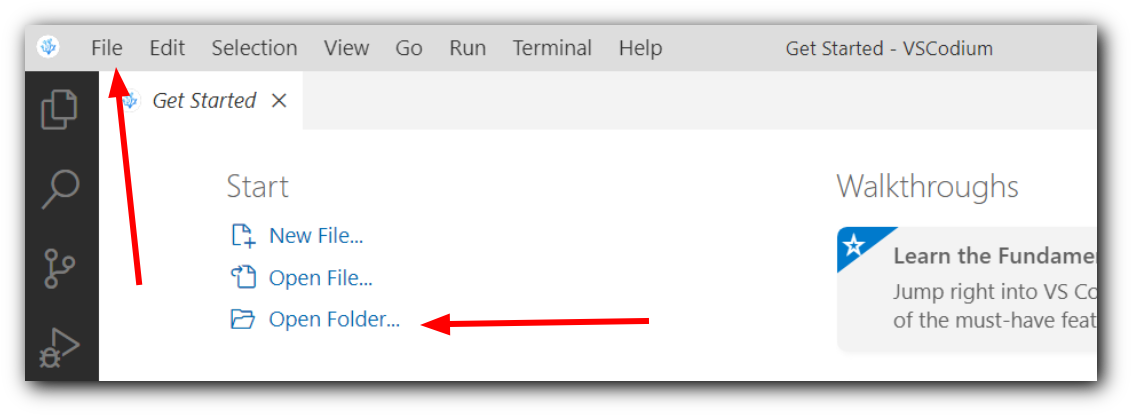
\includegraphics[width=.9\textwidth]{shots/installation/vscodium-folder01.png}

	\begin{multicols}{2}
	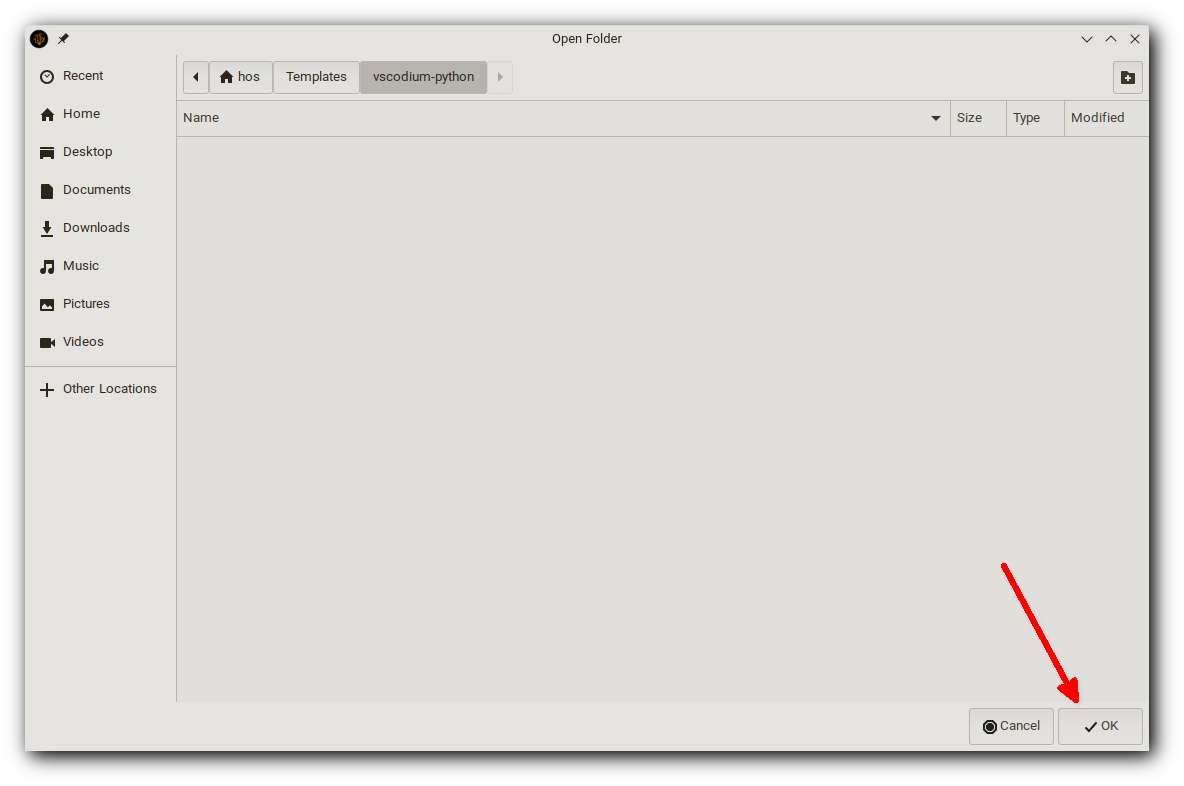
\includegraphics[width=.53\textwidth]{shots/installation/vscodium-folder02.png} \\
		\textit{Linux}

	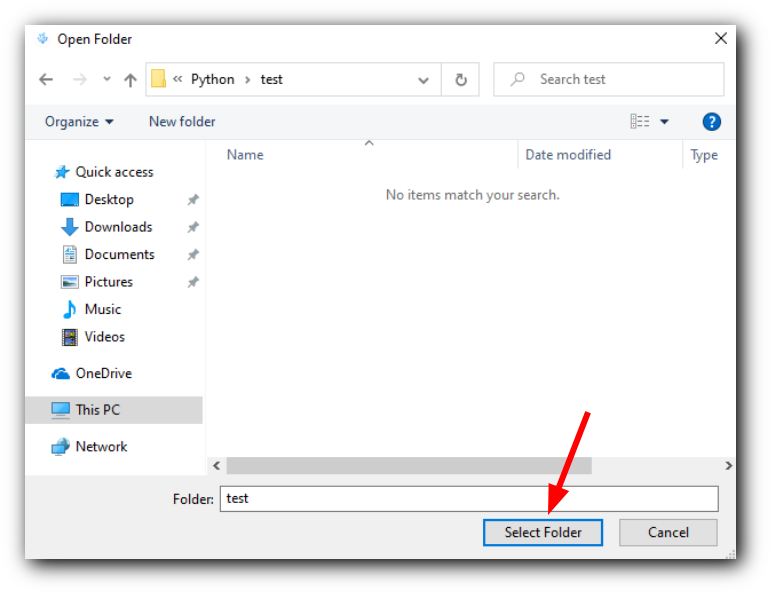
\includegraphics[width=.5\textwidth]{shots/installation/vscodium-folder02-win.png} \\
		\textit{Windows}
	\end{multicols}
\end{center}

Then you need to confirm that you trust the author
and the owner of this folder/directory:

\begin{center}
	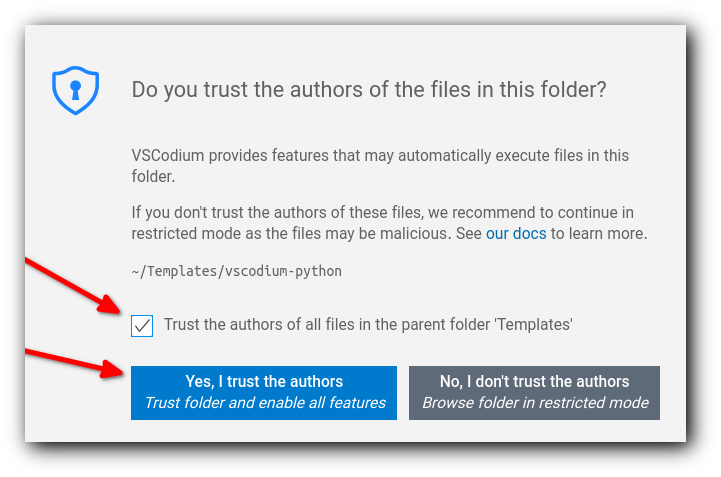
\includegraphics[width=.7\textwidth]{shots/installation/vscodium-folder03.png}
\end{center}

Now that you successfully opened a folder, it's time create a file:

\begin{center}
	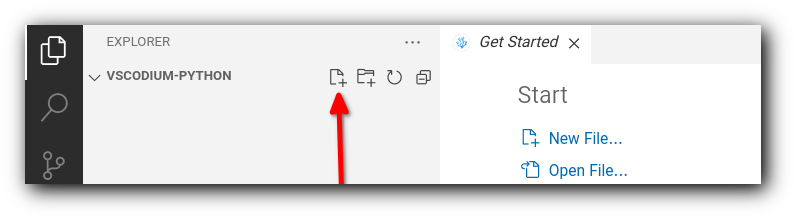
\includegraphics[width=.8\textwidth]{shots/installation/vscodium-folder04.png}

	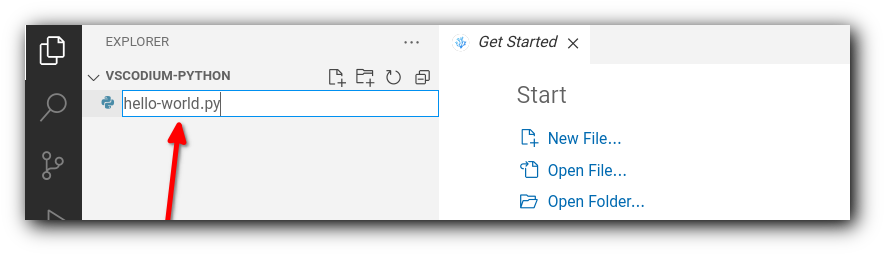
\includegraphics[width=.8\textwidth]{shots/installation/vscodium-folder05.png}
\end{center}

Now you can write and execute your python program.
Before we go further, let's check our python's version:

\begin{center}
	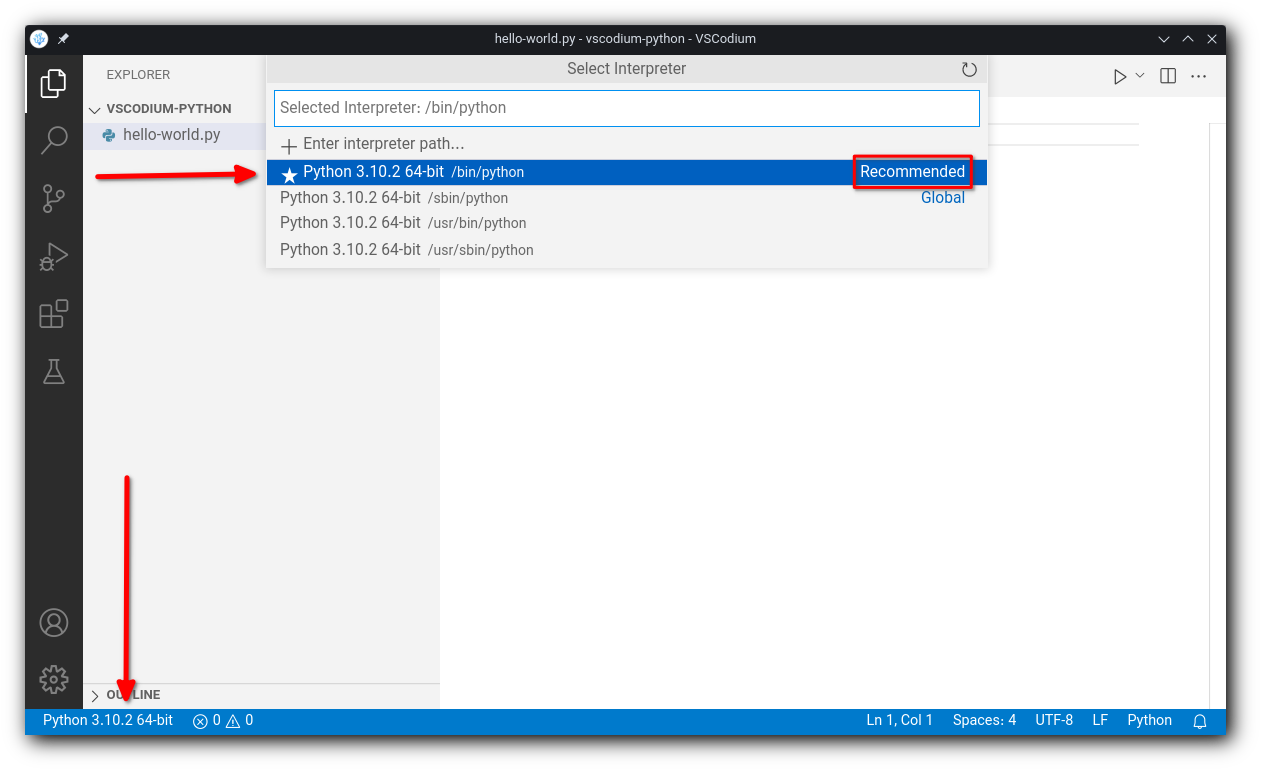
\includegraphics[width=.8\textwidth]{shots/installation/vscodium-python-version.png}
\end{center}


Alright! We are good to go and write our first Python program
and execute it:

\begin{center}
	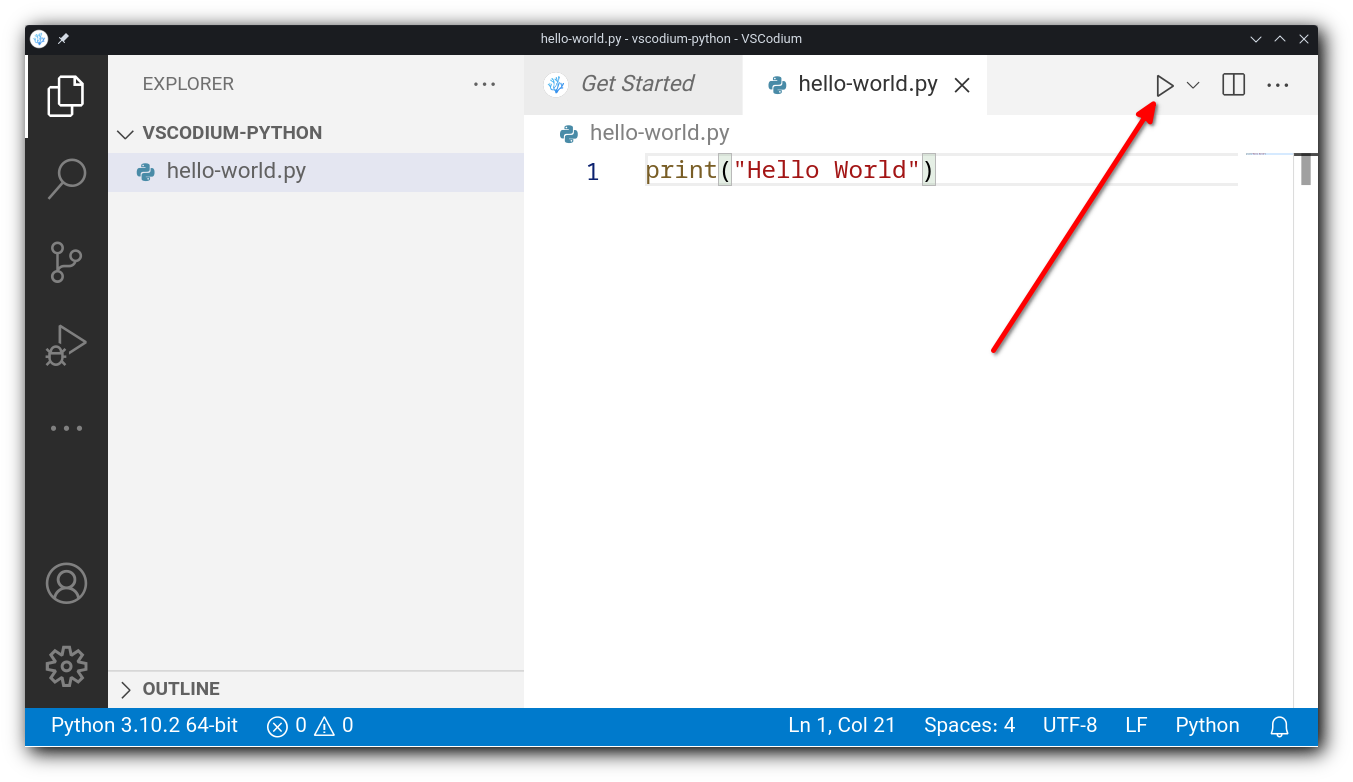
\includegraphics[width=.8\textwidth]{shots/installation/vscodium-run.png}

	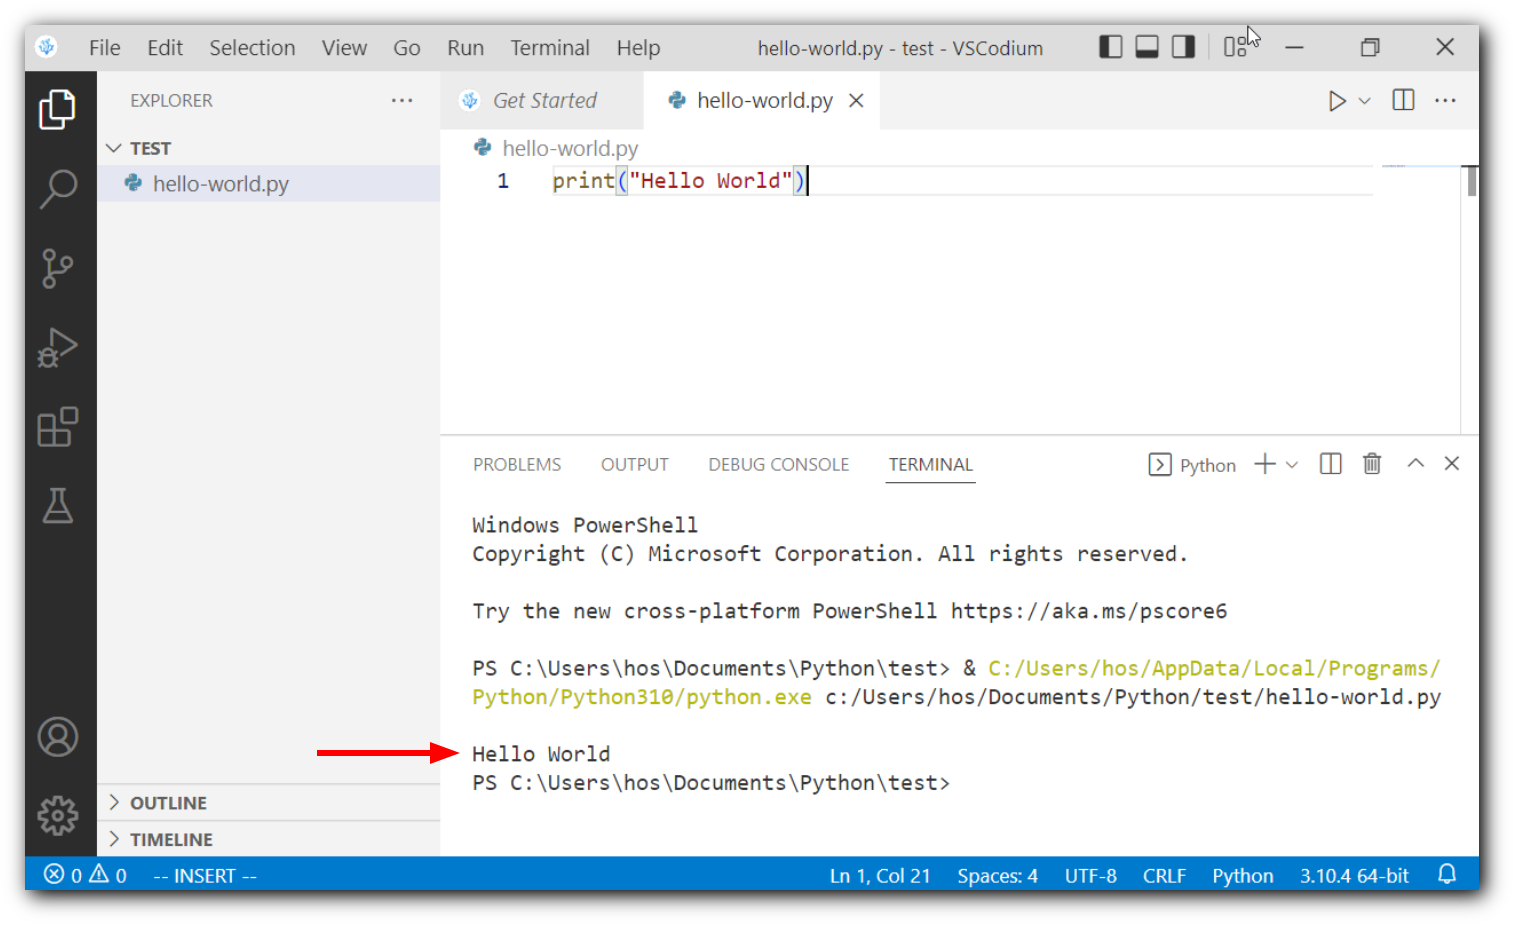
\includegraphics[width=.8\textwidth]{shots/installation/vscodium-run-output.png}
\end{center}
% }}}
% }}}
% quick start {{{
\subsection{Python Quickstart}
Python is an interpreted programming language, this means that as a developer
you write Python (\code{.py}) files in a text editor and then put those files into the
python interpreter to be executed.

The way to run a python file is like this on the command line:

\begin{vercode}
C:\Users\Your Name>python helloworld.py
\end{vercode}

Where \code{helloworld.py} is the name of your python file.

Let's write our first Python file, called \code{helloworld.py},
which can be done in any text editor.

\begin{ebox}
\begin{lstlisting}
print("Hello, World!")
\end{lstlisting}
\end{ebox}

Simple as that. Save your file. Open your command line, navigate to the
directory where you saved your file, and run:

\begin{vercode}
$ python helloworld.py_
\end{vercode}

The output should read:

\begin{vercode}
Hello, World!
$_
\end{vercode}

Congratulations, you have written and executed your first Python program.
% }}}
% python cli {{{
\subsection{The Python Command Line}
To test a short amount of code in python sometimes it is quickest and easiest
not to write the code in a file. This is made possible because Python can be
run as a command line itself.

Type the following on the Windows, Mac or Linux command line:

\begin{vercode}
$ python
\end{vercode}

From there you can write any python, including our hello world example from
earlier in the tutorial:

\begin{center}
	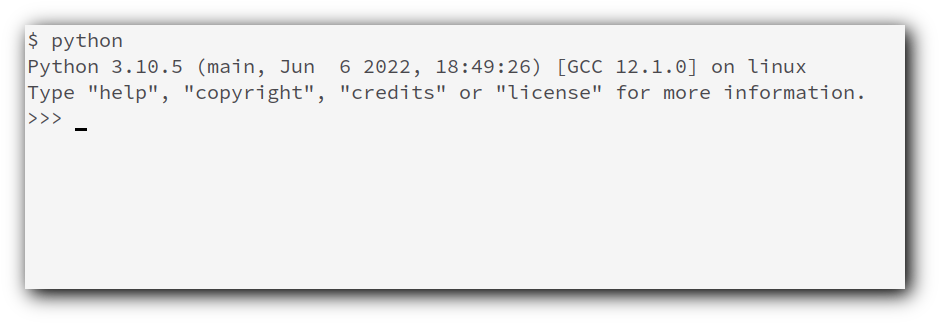
\includegraphics[width=.8\textwidth]{shots/getting_started/terminal.png}
\end{center}

Which will write ``Hello, World!" in the command line:

\begin{center}
	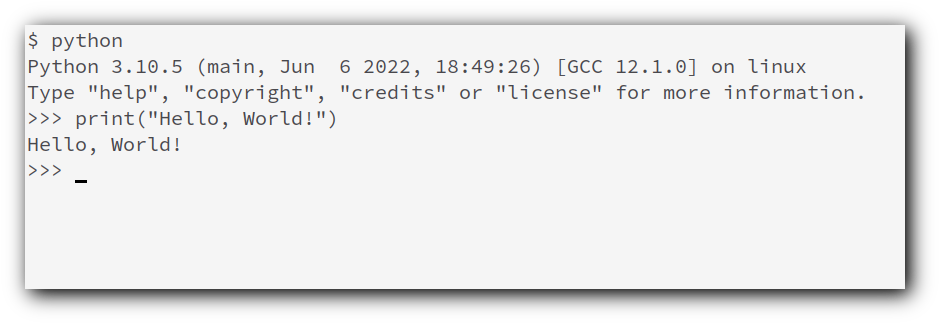
\includegraphics[width=.8\textwidth]{shots/getting_started/helloworld.png}
\end{center}

Whenever you are done in the python command line, you can simply type the
following to quit the python command line interface:

\begin{center}
	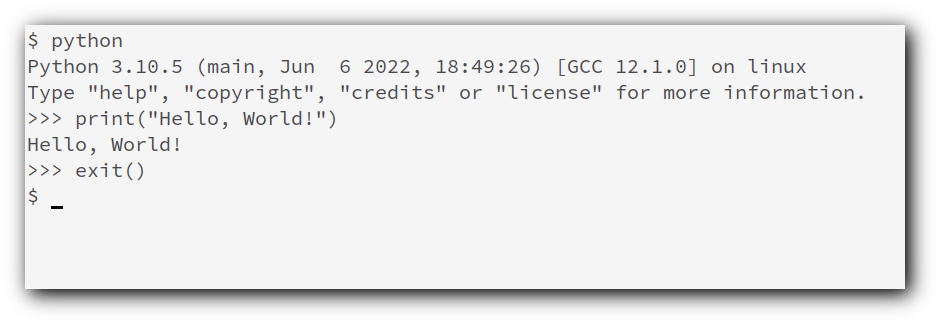
\includegraphics[width=.8\textwidth]{shots/getting_started/exitf.png}
\end{center}

% }}}
% }}}
%\vfill\newpage
% Syntax {{{
\section{Syntax}
% execute python syntax {{{
\subsection{Execute Python Syntax}
As we learned in the previous page, Python syntax can be executed by writing
directly in the Command Line:

\begin{ebox}
\begin{vercode}
>>> print("Hello, World!")
Hello, World!
\end{vercode}
\end{ebox}

Or by creating a python file on the server, using the .py file extension, and
running it in the Command Line:

\begin{ebox}
\begin{vercode}
C:\Users\Your Name> python myfile.py
\end{vercode}
\end{ebox}

Or on linux:

\begin{center}
	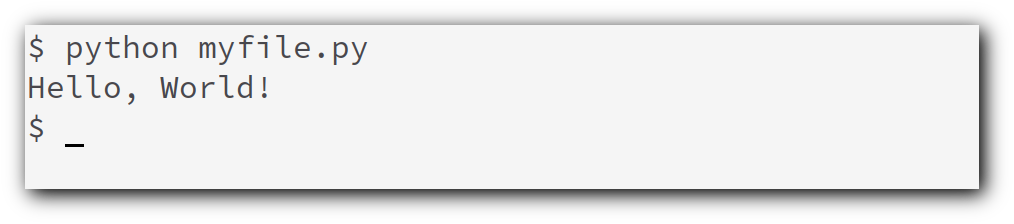
\includegraphics[width=.9\textwidth]{shots/getting_started/linux-run.png}
\end{center}
% }}}
% python indentation {{{
\subsection{Python Indentation}
Indentation refers to the spaces at the beginning of a code line.

Where in other programming languages the indentation in code is for readability
only, the indentation in Python is very important.

Python uses indentation to indicate a block of code.

\begin{ebox}
\begin{lstlisting}
if 5 > 2:
      print("Five is greater than two!")
\end{lstlisting}
\end{ebox}

Python will give you an error if you skip the indentation:

\begin{abox}
\begin{lstlisting}
if 5 > 2:
print("Five is greater than two!")
\end{lstlisting}
\end{abox}

The number of spaces is up to you as a programmer, the most common use is four,
but it has to be at least one.

\begin{ebox}
\begin{lstlisting}
if 5 > 2:
     print("Five is greater than two!")
if 5 > 2:
          print("Five is greater than two!")
\end{lstlisting}
\end{ebox}

You have to use the same number of spaces in the same block of code, otherwise
Python will give you an error:

\begin{abox}
\begin{lstlisting}
if 5 > 2:
     print("Five is greater than two!")
          print("Five is greater than two!")
\end{lstlisting}
\end{abox}
% }}}
% python variables {{{
\subsection{Python Variable}
In Python, variables are created when you assign a value to it:

\begin{ebox}
\begin{lstlisting}
x = 5
y = "Hello, World!"
\end{lstlisting}
\end{ebox}

Python has no command for declaring a variable.

You will learn more about variables in the chapter \ref{pyVariables}.
% }}}
% python comment {{{
\subsection{Comments}
Python has commenting capability for the purpose of in-code documentation.

Comments start with a \code{\#}, and Python will render the rest of the line as a comment:

\begin{ebox}
	\begin{lstlisting}
#This is a comment.
print("Hello, World!")
	\end{lstlisting}
\end{ebox}
% }}}
% test yourself {{{
\begin{tbox}
Insert the missing part of the code below to output ``Hello World".

\begin{lstlisting}[numbers=none]
`\wspace{1cm}`("Hello World")
\end{lstlisting}
\end{tbox}
% }}}
% }}}
\vfill\newpage
% Comments {{{
\section{Python Comments}
Comments can be used to explain Python code.

Comments can be used to make the code more readable.

Comments can be used to prevent execution when testing code.

% create {{{
\subsection{Creating a Comment}

Comments starts with a \code{\#}, and Python will ignore them:

\begin{ebox}
	\begin{lstlisting}
#This is a comment
print("Hello, World!")
	\end{lstlisting}
\end{ebox}

Comments can be placed at the end of a line, and Python will ignore the rest of
the line:

\begin{ebox}
	\begin{lstlisting}
print("Hello, World!") #This is a comment
	\end{lstlisting}
\end{ebox}

A comment does not have to be text that explains the code, it can also be used
to prevent Python from executing code:

\begin{ebox}
	\begin{lstlisting}
#print("Hello, World!")
print("Hello, World!")
	\end{lstlisting}
\end{ebox}
% }}}
% multiline comments {{{
\subsection{Multi Line Comments}
Python does not really have a syntax for multi line comments.

To add a multiline comment you could insert a \code{\#} for each line:

\begin{ebox}
	\begin{lstlisting}
#This is a comment
#written in
#more than just one line
print("Hello, World!")
	\end{lstlisting}
\end{ebox}

Or, not quite as intended, you can use a multiline string.

Since Python will ignore string literals that are not assigned to a variable,
you can add a multiline string (triple quotes) in your code, and place your
comment inside it:

\begin{ebox}
	\begin{lstlisting}
"""
This is a comment
written in
more than just one line
"""
print("Hello, World!")
	\end{lstlisting}
\end{ebox}

As long as the string is not assigned to a variable, Python will read the code,
but then ignore it, and you have made a multiline comment.

\begin{tbox}
Comments in Python are written with a special character, which one?

	\begin{lstlisting}[numbers=none]
`\wspace{5}`This is a comment
	\end{lstlisting}
\end{tbox}
% }}}
% }}}
\vfill\newpage
% Variables {{{
\section{Python Variables}\label{pyVariables}

% variables {{{
\subsection{Variables}

Variables are containers for storing data values.

% create {{{
\subsubsection{Creating Variables}

Python has no command for declaring a variable.

A variable is created the moment you first assign a value to it.

\begin{ebox}
	\begin{lstlisting}
x = 5
y = "John"
print(x)
print(y)
	\end{lstlisting}
\tcblower
	\begin{vercode}
5
John
	\end{vercode}
\end{ebox}

Variables do not need to be declared with any particular type, and can even
change type after they have been set.

Variables do not need to be declared with any particular type, and can even
change type after they have been set.

\begin{ebox}
	\begin{lstlisting}
x = 4			# x is of type int
x = "Sally"	# x is now of type str
print(x)
	\end{lstlisting}
\tcblower
	\begin{vercode}
Sally
	\end{vercode}
\end{ebox}
% }}}
% casting {{{
\subsubsection{Casting}

If you want to specify the data type of a variable, this can be done with casting.

\begin{ebox}
	\begin{lstlisting}
x = str(3)         # x will be '3' -> string
y = int(3)         # y will be 3 -> integer
z = float(3)       # z will be 3.0 -> float
	\end{lstlisting}
\end{ebox}
% }}}
% get type {{{
\subsubsection{Get the Type}
You can get the data type of a variable with the \code{type()} function.

\begin{ebox}
	\begin{lstlisting}
x = 5
y = "John"
print(type(x))
print(type(y))
	\end{lstlisting}
\tcblower
	\begin{vercode}
<class 'int'>
<class 'str'>
	\end{vercode}
\end{ebox}

\begin{nbox}
	You will learn more about \textit{data types} and \textit{casting} later in this tutorial.
\end{nbox}
% }}}
% single/double quotes {{{
\subsubsection{Single or Double Quotes?}
String variables can be declared either by using single or double quotes:

\begin{ebox}
	\begin{lstlisting}
x = "John"
# is the same as
x = 'John'
	\end{lstlisting}
\end{ebox}
% }}}
% case-sensetive {{{
\subsubsection{Case-Sensitive}

Variable names are case-sensitive.

\begin{ebox}
	\begin{lstlisting}
a = 4
A = "Sally"
#A will not overwrite a
	\end{lstlisting}
\end{ebox}
% }}}
% }}}
% Var Names {{{
\subsection{Variable Names}
A variable can have a short name (like x and y)\\
or a more descriptive name
(age, carname, total\_volume).
Rules for Python variables:

\begin{itemize}
	\item A variable name must start with a letter or the underscore character
	\item A variable name cannot start with a number
	\item A variable name can only contain alpha-numeric characters and underscores (A-z, 0-9, and \_ )
	\item Variable names are case-sensitive (age, Age and AGE are three different variables)
\end{itemize}

\begin{ebox}
	\begin{lstlisting}
myvar = "John"
my_var = "John"
_my_var = "John"
myVar = "John"
MYVAR = "John"
myvar2 = "John"
	\end{lstlisting}
\end{ebox}

\begin{abox}
	\begin{lstlisting}
2myvar = "John"
my-var = "John"
my var = "John"
	\end{lstlisting}
\end{abox}

\begin{nbox}
	Remember that variable names are \textit{case-sensitive}
\end{nbox}
% }}}
% Multi Words Variable Names {{{
\subsection{Multi Words Variable Names}
Variable names with more than one word can be difficult to read.

There are several techniques you can use to make them more readable:

\subsubsection{Camel Case}

Each word, except the first, starts with a capital letter:

\begin{ebox}
	\begin{lstlisting}
 myVariableName = "John"
	\end{lstlisting}
\end{ebox}

\subsubsection{Pascal Case}

Each word starts with a capital letter:

\begin{ebox}
	\begin{lstlisting}
 MyVariableName = "John"
	\end{lstlisting}
\end{ebox}

\subsubsection{Snake Case}

Each word is separated by an underscore character:

\begin{ebox}
	\begin{lstlisting}
 my_variable_name = "John"
	\end{lstlisting}
\end{ebox}
% }}}
% Assign Multiple Values {{{
\subsection{Assign Multiple Values}

% Many Values to Multiple Variables {{{
\subsubsection{Many Values to Multiple Variables}

Python allows you to assign values to multiple variables in one line:

\begin{ebox}
	\begin{lstlisting}
x, y, z = "Orange", "Banana", "Cherry"
print(x)
print(y)
print(z)
	\end{lstlisting}
\tcblower
	\begin{vercode}
Orange
Banana
Cherry
	\end{vercode}
\end{ebox}

\begin{nbox}
	Make sure the number of variables matches the number of values, or else you
	will get an error.
\end{nbox}
% }}}
% One Value to Multiple Variables {{{
\subsubsection{One Value to Multiple Variables}

And you can assign the same value to multiple variables in one line:

\begin{ebox}
	\begin{lstlisting}
x = y = z = "Orange"
print(x)
print(y)
print(z)
	\end{lstlisting}
\tcblower
	\begin{vercode}
Orange
Orange
Orange
	\end{vercode}
\end{ebox}
% }}}
% Unpack a Collection {{{
\subsubsection{Unpack a Collection}

If you have a collection of values in a list, tuple etc. Python allows you to
extract the values into variables. This is called unpacking.

\begin{ebox}
	\begin{lstlisting}
fruits = ["apple", "banana", "cherry"]
x, y, z = fruits
print(x)
print(y)
print(z)
	\end{lstlisting}
\tcblower
	\begin{vercode}
apple
banana
cherry
	\end{vercode}
\end{ebox}

You will learn more about this in chapter \ref{pyUnpackTuple}.
% }}}

% }}}
% Output Variables {{{
\subsection{Output Variables}

\subsubsection{Output Variables}

The Python \code{print()} function is often used to output variables.

\begin{ebox}
	\begin{lstlisting}
x = "Python is awesome"
print(x)
	\end{lstlisting}
\tcblower
	\begin{vercode}
Python is awesome
	\end{vercode}
\end{ebox}

In the \code{print()} function, you output multiple variables, separated by a comma:

\begin{ebox}
	\begin{lstlisting}
x = "Python"
y = "is"
z = "awesome"
print(x, y, z)
	\end{lstlisting}
\tcblower
	\begin{vercode}
Python is awesome
	\end{vercode}
\end{ebox}

You can also use the \code{+} operator to output multiple variables:

\begin{ebox}
	\begin{lstlisting}
x = "Python "
y = "is "
z = "awesome"
print(x + y + z)
	\end{lstlisting}
\tcblower
	\begin{vercode}
Python is awesome
	\end{vercode}
\end{ebox}

\begin{nbox}
	Notice the space character after ``Python " and ``is ", without them the
	result would be \\ ``Pythonisawesome".
\end{nbox}

For numbers, the \code{+} character works as a mathematical operator:

\begin{ebox}
	\begin{lstlisting}
x = 5
y = 10
print(x + y)
	\end{lstlisting}
\tcblower
	\begin{vercode}
15
	\end{vercode}
\end{ebox}

In the \code{print()} function, when you try to combine a string and a number with the
\code{+} operator, Python will give you an error:

\begin{abox}
	\begin{lstlisting}
x = 5
y = "John"
print(x + y)
	\end{lstlisting}
\tcblower
	\begin{vercode}
Traceback (most recent call last):
  File "/home/hos/Documents/teach/python/en/test.py",
  line 3, in <module>
    print(x + y)
TypeError: unsupported operand type(s) for +: 'int' and 'str'
	\end{vercode}
\end{abox}

The best way to output multiple variables in the \code{print()} function is to
separate them with commas, which even support different data types:

\begin{ebox}
	\begin{lstlisting}
x = 5
y = "John"
print(x, y)
	\end{lstlisting}
\tcblower
	\begin{vercode}
5 John
	\end{vercode}
\end{ebox}

% }}}
% Global Variables {{{
\subsection{Global Variables}

% Global Variables {{{
\subsubsection{Global Variables}

Variables that are created outside of a function
(as in all of the examples above)
are known as global variables.

Global variables can be used by everyone, both inside of functions and outside.

\begin{ebox}
	\begin{lstlisting}
x = "awesome"

def myfunc():
    print("Python is " + x)

myfunc()
	\end{lstlisting}
\tcblower
	\begin{vercode}
Python is awesome
	\end{vercode}
\end{ebox}

If you create a variable with the same name inside a function, this variable
will be local, and can only be used inside the function. The global variable
with the same name will remain as it was, global and with the original value.

\begin{ebox}
	\begin{lstlisting}
x = "awesome"

def myfunc():
    x = "fantastic"
    print("Python is " + x)

myfunc()

print("Python is " + x)
	\end{lstlisting}
\tcblower
	\begin{vercode}
Python is fantastic
Python is awesome
	\end{vercode}
\end{ebox}
% }}}
% The global Keyword {{{
\subsubsection{The \textit{global} Keyword}

Normally, when you create a variable inside a function, that variable is local,
and can only be used inside that function.

To create a global variable inside a function, you can use the \code{global} keyword.

\begin{ebox}
	If you use the global keyword, the variable belongs to the global scope:

	\begin{lstlisting}
def myfunc():
    global x
    x = "fantastic"

myfunc()

print("Python is " + x)
	\end{lstlisting}
\tcblower
	\begin{vercode}
Python is fantastic
	\end{vercode}
\end{ebox}

Also, use the \code{global} keyword if you want to change a global variable
inside a function.

\begin{ebox}
	To change the value of a global variable inside a function, refer to the
	variable by using the \code{global} keyword:

	\begin{lstlisting}
x = "awesome"

def myfunc():
    global x
    x = "fantastic"

myfunc()

print("Python is " + x)
	\end{lstlisting}
\tcblower
	\begin{vercode}
Python is fantastic
	\end{vercode}
\end{ebox}

% }}}
% }}}
% Exercises {{{
\subsection{Test Yourself With Exercises}

Now you have learned a lot about variables, and how to use them in Python.

Are you ready for a test?

Try to insert the missing part to make the code work as expected:

\begin{tbox}
Create a variable named \code{carname} and assign the value \code{Volvo} to it.

	\begin{lstlisting}[numbers=none]
`\wspace{carname}` = "`\wspace{Volvo}`"
	\end{lstlisting}
\end{tbox}
% }}}
% }}}
\vfill\newpage
% Data Types {{{
\section{Data Types}

% Built-in Data Types {{{
\subsection{Built-in Data Types}

In programming, data type is an important concept.

Variables can store data of different types, and different types can do different things.

Python has the following data types built-in by default, in these categories:

\begin{table}[h]
	%\begin{center}
		\begin{tabular}{ll}
			\tcol{Test type:}{\lcode{str}}
			\tcol{Numeric type:}{\lcode{int}, \lcode{float}, \lcode{complex}}
			\tcol{Sequence Types:}{\lcode{list}, \lcode{tuple}, \lcode{range}}
			\tcol{Mapping Type:}{\lcode{dict}}
			\tcol{Set Types:}{\lcode{set}, \lcode{frozenset}}
			\tcol{Boolean Type:}{\lcode{bool}}
			\tcol{Binary Types:}{\lcode{bytes}, \lcode{bytearray}, \lcode{memoryview}}
			\tcol{None Type:}{\lcode{NoneType}}
		\end{tabular}
	%\end{center}
\end{table}
% }}}
% Getting the Data Type {{{
\subsection{Getting the Data Type}

You can get the data type of any object by using the \code{type()} function:

\begin{ebox}
Print the data type of the variable x:

	\begin{lstlisting}
x = 5
print(type(x))
	\end{lstlisting}

\tcblower
	\begin{vercode}
<class 'int'>
	\end{vercode}
\end{ebox}
% }}}
% Setting the Data Type {{{
\vfill\newpage
\subsection{Setting the Data Type}

In Python, the data type is set when you assign a value to a variable:

\begin{table}[h]
	\begin{center}
		\begin{tabularx}{.85\textwidth}{Xll}
\textbf{Example} & \textbf{Data Type} \\
	\tcol{\lcode{x = "Hello World"} }{\lcode{str}}
	\tcol{\lcode{x = 20}}{\lcode{int}}
	\tcol{\lcode{x = 20.5}}{\lcode{float}}
	\tcol{\lcode{x = 1j}}{\lcode{complex}}
	\tcol{\lcode{x = ["apple", "banana", "cherry"]}}{\lcode{list}}
	\tcol{\lcode{x = ("apple", "banana", "cherry")}}{\lcode{tuple}}
	\tcol{\lcode{x = range(6)} }{\lcode{range}}
	\tcol{\lcode{x = {"name" : "John", "age" : 36}} }{\lcode{dict}}
	\tcol{\lcode{x = {"apple", "banana", "cherry"}} }{\lcode{set}}
	%\tcol{\lcode{x = frozenset({"apple", "banana", "cherry"})}}{\lcode{frozenset}}
	\tcol{\lcode{x = frozenset(\{"apple", "banana", "cherry"\})}}{\lcode{frozenset}}
	\tcol{\lcode{x = True}}{\lcode{bool}}
	\tcol{\lcode{x = b"Hello"} }{\lcode{bytes}}
	\tcol{\lcode{x = bytearray(5)} }{\lcode{bytearray}}
	\tcol{\lcode{x = memoryview(bytes(5))} }{\lcode{memoryview}}
	\tcol{\lcode{x = None}}{\lcode{NoneType}}
		\end{tabularx}
	\end{center}
\end{table}
% }}}
% Setting the Specific Data Type {{{
\subsection{Setting the Specific Data Type}

If you want to specify the data type, you can use the following constructor
functions:

\begin{table}[h]
	\begin{center}
		\begin{tabularx}{.85\textwidth}{Xll}
\textbf{Example} & \textbf{Data Type} \\
	\tcol{\lcode{x = str("Hello World")}}{\lcode{str}}
	\tcol{\lcode{x = int(20)}}{\lcode{int}}
	\tcol{\lcode{x = float(20.5)}}{\lcode{float}}
	\tcol{\lcode{x = complex(1j)}}{\lcode{complex}}
	\tcol{\lcode{x = list(("apple", "banana", "cherry"))}}{\lcode{list}}
	\tcol{\lcode{x = tuple(("apple", "banana", "cherry"))}}{\lcode{tuple}}
	\tcol{\lcode{x = range(6)}}{\lcode{range}}
	\tcol{\lcode{x = dict(name="John", age=36)}}{\lcode{dict}}
	\tcol{\lcode{x = set(("apple", "banana", "cherry"))}}{\lcode{set}}
	\tcol{\lcode{x = frozenset(("apple", "banana", "cherry"))}}{\lcode{frozenset}}
	\tcol{\lcode{x = bool(5)}}{\lcode{bool}}
	\tcol{\lcode{x = bytes(5)}}{\lcode{bytes}}
	\tcol{\lcode{x = bytearray(5)}}{\lcode{bytearray}}
	\tcol{\lcode{x = memoryview(bytes(5))}}{\lcode{memoryview}}
		\end{tabularx}
	\end{center}
\end{table}
% }}}
% Test {{{
\subsection{Exercise}
\begin{tbox}
The following code example would print the data type of x, what data type would that be?

\begin{lstlisting}[numbers=none]
x = 5
print(type(x))
	\end{lstlisting}
\tcblower
	\begin{lstlisting}[numbers=none]
`\wspace{<class 'int'>}`
	\end{lstlisting}
\end{tbox}
% }}}
% }}}
\vfill\newpage
% Numbers {{{
\section{Numbers}
% Python Numbers {{{
\subsection{Python Numbers}

There are three numeric types in Python:

\begin{itemize}
	\item \code{int}
	\item \code{float}
	\item \code{complex}
\end{itemize}

Variables of numeric types are created when you assign a value to them:

\begin{ebox}
	\begin{lstlisting}
x = 1		# int
y = 2.8		# float
z = 1j		# complex
	\end{lstlisting}
\end{ebox}

To verify the type of any object in Python,
use the \code{type()} function:

\begin{ebox}
	\begin{lstlisting}
print(type(x))
print(type(y))
print(type(z))
	\end{lstlisting}
\tcblower
	\begin{vercode}
<class 'int'>
<class 'float'>
<class 'complex'>
	\end{vercode}
\end{ebox}

% }}}
% Int {{{
\subsection{Int}
Int, or integer, is a whole number, positive or negative, without
decimals, of unlimited length.

\begin{ebox}
	\begin{lstlisting}
x = 1
y = 35656222554887711
z = -3255522

print(type(x))
print(type(y))
print(type(z))
	\end{lstlisting}
\tcblower
	\begin{vercode}
<class 'int'>
<class 'int'>
<class 'int'>
	\end{vercode}
\end{ebox}
% }}}
% Float {{{
\subsection{Float}
Float, or ``floating point number" is a number, positive or negative,
containing one or more decimals.

\begin{ebox}
	\begin{lstlisting}
x = 1.10
y = 1.0
z = -35.59

print(type(x))
print(type(y))
print(type(z))
	\end{lstlisting}
\tcblower
	\begin{vercode}
<class 'float'>
<class 'float'>
<class 'float'>
	\end{vercode}
\end{ebox}

Float can also be scientific numbers with
an "e" to indicate the power of 10.

\begin{ebox}
	\begin{lstlisting}
x = 35e3
y = 12E4
z = -87.7e100

print(type(x))
print(type(y))
print(type(z))
	\end{lstlisting}
\tcblower
	\begin{vercode}
<class 'float'>
<class 'float'>
<class 'float'>
	\end{vercode}
\end{ebox}
% }}}
% Complex {{{
\subsection{Complex}

Complex numbers are written with a "j" as the imaginary part:

\begin{ebox}
	\begin{lstlisting}
x = 3+5j
y = 5j
z = -5j

print(type(x))
print(type(y))
print(type(z))
	\end{lstlisting}
\tcblower
	\begin{vercode}
<class 'complex'>
<class 'complex'>
<class 'complex'>
	\end{vercode}
\end{ebox}
% }}}
% Type Conversion {{{
\subsubsection{Type Conversion}
You can convert from one type to another with the
\code{int()}, \code{float()},
and \code{complex()} methods:

\begin{ebox}
Convert from one type to another:
	\begin{lstlisting}
x = 1		# int
y = 2.8		# float
z = 1j		# complex

#convert from int to float:
a = float(x)

#convert from float to int:
b = int(y)

#convert from int to complex:
c = complex(x)

print(a)
print(b)
print(c)

print(type(a))
print(type(b))
print(type(c))
	\end{lstlisting}
\tcblower
	\begin{vercode}
1.0
2
(1+0j)
<class 'float'>
<class 'int'>
<class 'complex'>
	\end{vercode}
\end{ebox}

\begin{nbox}
You cannot convert complex numbers into another number type.
\end{nbox}
% }}}
% Random Number {{{
\subsection{Random Number}
Python does not have a \code{random()} function to make
a random number, but Python has a built-in module
called \code{random} that can be used to make random numbers:

\begin{ebox}
Import the random module,
and display a random number between 1 and 9:
	\begin{lstlisting}
import random

print(random.randrange(1, 10))
	\end{lstlisting}
\tcblower
	\begin{vercode}
4
	\end{vercode}
\end{ebox}
% }}}
% Test {{{
\subsection{Exercise}
\begin{tbox}
Insert the correct syntax to convert x into a floating point number.

\begin{lstlisting}[numbers=none]
x = 5
x = `\wspace{float}`(x)
\end{lstlisting}
\end{tbox}
% }}}
% }}}
\vfill\newpage
% Casting {{{
\section{Python Casting}
% Specify a Variable Type {{{
\subsection{Specify a Variable Type}
There may be times when you want to specify a type on to a variable. This can
be done with casting. Python is an object-orientated language, and as such it
uses classes to define data types, including its primitive types.

Casting in python is therefore done using constructor functions:

\begin{itemize}
	\item \code{int()} - constructs an integer number from an integer literal,
		a float literal (by removing all decimals), or a string literal
		(providing the string represents a whole number)
	\item \code{float()} - constructs a float number from an integer literal, a
		float literal or a string literal (providing the string represents a
		float or an integer)
	\item \code{str()} - constructs a string from a wide variety of data types,
		including strings, integer literals and float literals
\end{itemize}

\begin{ebox}
	Integers:
	\begin{lstlisting}
x = int(1)			# x will be 1
y = int(2.8)		# y will be 2
z = int("3")		# z will be 3
	\end{lstlisting}

	Floats:
	\begin{lstlisting}
x = float(1)			# x will be 1.0
y = float(2.8)			# y will be 2.8
z = float("3")			# z will be 3.0
w = float("4.2")		# w will be 4.2
	\end{lstlisting}

	Strings:
	\begin{lstlisting}
x = str("s1")		# x will be 's1'
y = str(2)			# y will be '2'
z = str(3.0)		# z will be '3.0'
	\end{lstlisting}

\end{ebox}
% }}}
% }}}
\vfill\newpage
% Strings {{{
\section{Python Strings}
% Strings {{{
\subsection{Strings}
Strings in python are surrounded by either single quotation marks, or double
quotation marks.

\code{'Hello'} is the same as \code{"Hello"}.

You can display a string literal with the \code{print()} function:

\begin{ebox}
	\begin{lstlisting}
print("Hello")
print('Hello')
	\end{lstlisting}
\tcblower
	\begin{vercode}
Hello
Hello
	\end{vercode}
\end{ebox}

% Assign String to a Variable {{{
\subsubsection{Assign String to a Variable}

Assigning a string to a variable is done with the variable name followed by an
equal sign and the string:

\begin{ebox}
	\begin{lstlisting}
a = "Hello"
print(a)
	\end{lstlisting}
\tcblower
	\begin{vercode}
Hello
	\end{vercode}
\end{ebox}
% }}}
% Multiline Strings {{{
\subsubsection{Multiline Strings}

You can assign a multiline string to a variable by using three quotes:

\begin{ebox}
You can use three double quotes:

	\begin{lstlisting}
a = """Lorem ipsum dolor sit amet,
consectetur adipiscing elit,
sed do eiusmod tempor incididunt
ut labore et dolore magna aliqua."""
print(a)
	\end{lstlisting}

Or three single quotes:

	\begin{lstlisting}
a = '''Lorem ipsum dolor sit amet,
consectetur adipiscing elit,
sed do eiusmod tempor incididunt
ut labore et dolore magna aliqua.'''
print(a)
	\end{lstlisting}
\tcblower
	\begin{vercode}
Lorem ipsum dolor sit amet,
consectetur adipiscing elit,
sed do eiusmod tempor incididunt
ut labore et dolore magna aliqua.
	\end{vercode}
\end{ebox}

\begin{nbox}
in the result, the line breaks are inserted at the same position as in the
code.
\end{nbox}
% }}}
% Strings are Arrays {{{
\subsubsection{Strings are Arrays}
Like many other popular programming languages, strings in Python are arrays of
bytes representing unicode characters.

However, Python does not have a character data type, a single character is
simply a string with a length of 1.

Square brackets can be used to access elements of the string.

\begin{ebox}
Get the character at position 1 (remember that the first character has the position 0):

	\begin{lstlisting}
a = "Hello, World!"
print(a[1])
	\end{lstlisting}
\tcblower
	\begin{vercode}
e
	\end{vercode}
\end{ebox}
% }}}
% Looping Through a String {{{
\subsubsection{Looping Through a String}

Since strings are arrays, we can loop through the characters in a string, with
a \code{for} loop.

\begin{ebox}
Loop through the letters in the word ``banana":

	\begin{lstlisting}
for x in "banana":
    print(x)
	\end{lstlisting}
\tcblower
	\begin{vercode}
b
a
n
a
n
a
	\end{vercode}
\end{ebox}

\begin{itemize}
	\item Learn more about \code{for} Loops in chapter \ref{pyForLoop}.
\end{itemize}
% }}}
% String Length {{{
\subsubsection{String Length}

To get the length of a string, use the \code{len()} function.

\begin{ebox}
The \code{len()} function returns the length of a string:
	\begin{lstlisting}
a = "Hello, World!"
print(len(a))
	\end{lstlisting}
\tcblower
	\begin{vercode}
13
	\end{vercode}
\end{ebox}
% }}}
% Check String {{{
\subsubsection{Check String}

To check if a certain phrase or character is present in a string,
we can use the keyword \code{in}.

\begin{ebox}
Check if ``free" is present in the following text:
	\begin{lstlisting}
txt = "The best things in life are free!"
print("free" in txt)
	\end{lstlisting}
\tcblower
	\begin{vercode}
True
	\end{vercode}
\end{ebox}

Use it in an \code{if} statement:

\begin{ebox}
	\begin{lstlisting}
txt = "The best things in life are free!"
if "free" in txt:
    print("Yes, 'free' is present.")
	\end{lstlisting}
\tcblower
	\begin{vercode}
Yes, 'free' is present.
	\end{vercode}
\end{ebox}

\begin{itemize}
	\item Learn more about \code{if} statements in chapter \ref{pyIfStatement}
\end{itemize}
% }}}
% Check if NOT {{{
\subsubsection{Check if NOT}
To check if a certain phrase or character is NOT present in a string, we can
use the keyword \code{not in}.

\begin{ebox}
Check if ``expensive" is NOT present in the following text:

	\begin{lstlisting}
txt = "The best things in life are free!"
print("expensive" not in txt)
	\end{lstlisting}
\tcblower
	\begin{vercode}
True
	\end{vercode}
\end{ebox}

Use it in an \code{if} statement:

\begin{ebox}
print only if ``expensive" is NOT present:

	\begin{lstlisting}
txt = "The best things in life are free!"
if "expensive" not in txt:
    print("No, 'expensive' is NOT present.")
	\end{lstlisting}
\tcblower
	\begin{vercode}
No, 'expensive' is NOT present.
	\end{vercode}
\end{ebox}

% }}}
% }}}
% Slicing Strings {{{
\subsection{Slicing Strings}
You can return a range of characters by using the slice syntax.

Specify the start index and the end index, separated by a colon, to return a
part of the string.

\begin{ebox}
	Get the characters from position 2 to position 5 (not included):

	\begin{lstlisting}
b = "Hello, World!"
print(b[2:5])
	\end{lstlisting}
\tcblower
	\begin{vercode}
llo
	\end{vercode}
\end{ebox}

\begin{nbox}
	The first character has index 0.
\end{nbox}
% Slice From the Start {{{
\subsubsection{Slice From the Start}

By leaving out the start index, the range will start at the first character:

\begin{ebox}
	Get the characters from the start to position 5 (not included):
	\begin{lstlisting}
b = "Hello, World!"
print(b[:5])
	\end{lstlisting}
\tcblower
	\begin{vercode}
Hello
	\end{vercode}
\end{ebox}
% }}}
% Slice To the End {{{
\subsubsection{Slice To the End}

By leaving out the end index, the range will go to the end:

\begin{ebox}
Get the characters from position 2, and all the way to the end:
	\begin{lstlisting}
b = "Hello, World!"
print(b[2:])
	\end{lstlisting}
\tcblower
	\begin{vercode}
llo, World!
	\end{vercode}
\end{ebox}
% }}}
% Negative Indexing {{{
\subsubsection{Negative Indexing}

Use negative indexes to start the slice from the end of the string:

\begin{ebox}{%\sffamily

Get the characters:

\hspace{5mm}
From: ``o" in ``World!" (position -5)

\hspace{5mm}
To, but not included: ``d" in ``World!" (position -2):
}
	\begin{lstlisting}
b = "Hello, World!"
print(b[-5:-2])
	\end{lstlisting}
\tcblower
	\begin{vercode}
orl
	\end{vercode}
\end{ebox}
% }}}
% }}}
% Modify Strings {{{
\subsection{Modify Strings}

Python has a set of built-in methods that you can use on strings.

% Upper Case {{{
\begin{ebox}
The \code{upper()} method returns the string in upper case:

	\begin{lstlisting}
a = "Hello, World!"
print(a.upper())
	\end{lstlisting}
\tcblower
	\begin{vercode}
HELLO, WORLD!
	\end{vercode}
\end{ebox}
% }}}
% Lower Case {{{
\subsubsection{Lower Case}
\begin{ebox}
The \code{lower()} method returns the string in lower case:

	\begin{lstlisting}
a = "Hello, World!"
print(a.lower())
	\end{lstlisting}
\tcblower
	\begin{vercode}
hello, world!
	\end{vercode}
\end{ebox}
% }}}
% Remove Whitespace {{{
\subsubsection{Remove Whitespace}
Whitespace is the space before and/or after the actual text, and very often you
want to remove this space.

\begin{ebox}
The \code{strip()} method removes any whitespace from the beginning or the end:

	\begin{lstlisting}
a = " Hello, World! "
print(a.strip())		# returns "Hello, World!"
	\end{lstlisting}
\tcblower
	\begin{vercode}
Hello, World!
	\end{vercode}
\end{ebox}
% }}}
% Replace String {{{
\subsubsection{Replace String}

\begin{ebox}
The \code{replace()} method replaces a string with another string:

	\begin{lstlisting}
a = "Hello, World!"
print(a.replace("H", "J"))
	\end{lstlisting}
\tcblower
	\begin{vercode}
Jello, World!
	\end{vercode}
\end{ebox}
% }}}
% Split String {{{
\subsubsection{Split String}

The \code{split()} method returns a list where the text between the specified
separator becomes the list items.

\begin{ebox}
The \code{split()} method splits the string into substrings if it finds instances of the separator:

	\begin{lstlisting}
a = "Hello, World!"
print(a.split(","))     # returns ['Hello', ' World!']
	\end{lstlisting}
\tcblower
	\begin{vercode}
['Hello', ' World!']
	\end{vercode}
\end{ebox}

\begin{itemize}
	\item Learn more about Lists in chapter \ref{pyLists}.
\end{itemize}
% }}}
% }}}
% String Concatenation {{{
\subsection{String Concatenation}
To concatenate, or combine, two strings you can use the \code{+} operator.

\begin{ebox}
Merge variable \code{a} with variable \code{b} into variable \code{c}:

	\begin{lstlisting}
a = "Hello"
b = "World"
c = a + b
print(c)
	\end{lstlisting}
\tcblower
	\begin{vercode}
HelloWorld
	\end{vercode}
\end{ebox}

\begin{ebox}
To add a space between them, add a \code{" "}:

	\begin{lstlisting}
a = "Hello"
b = "World"
c = a + " " + b
print(c)
	\end{lstlisting}
\tcblower
	\begin{vercode}
Hello World
	\end{vercode}
\end{ebox}
% }}}
% Format Strings {{{
\subsection{Format Strings}
As we learned in the Python Variables chapter, we cannot combine strings and
numbers like this:

\begin{abox}
	\begin{lstlisting}
age = 36
txt = "My name is John, I am " + age
print(txt)
	\end{lstlisting}
\end{abox}

But we can combine strings and numbers by using the \code{format()} method!

The \code{format()} method takes the passed arguments, formats them, and places them
in the string where the placeholders \code{\{\}} are:

\begin{ebox}
Use the \code{format()} method to insert numbers into strings:

	\begin{lstlisting}
age = 36
txt = "My name is John, and I am {}"
print(txt.format(age))
	\end{lstlisting}
\tcblower
	\begin{vercode}
My name is John, and I am 36
	\end{vercode}
\end{ebox}

The \lcode{format()} method takes unlimited number of arguments, and are placed into
the respective placeholders:

\begin{ebox}

	\begin{lstlisting}
quantity = 3
itemno = 567
price = 49.95
myorder = "I want {} pieces of item {} for {} dollars."
print(myorder.format(quantity, itemno, price))
	\end{lstlisting}
\tcblower
	\begin{vercode}
I want 3 pieces of item 567 for 49.95 dollars.
	\end{vercode}
\end{ebox}

You can use index numbers \code{\{0\}} to be sure the arguments are placed in the correct placeholders:

\begin{ebox}
	\begin{lstlisting}
quantity = 3
itemno = 567
price = 49.95
myorder = "I want to pay {2} dollars for {0} pieces of item {1}."
print(myorder.format(quantity, itemno, price))
	\end{lstlisting}
\tcblower
	\begin{vercode}
I want to pay 49.95 dollars for 3 pieces of item 567.
	\end{vercode}
\end{ebox}

\begin{itemize}
	\item Learn more about String Formatting in chapter \ref{pyStringFormat}
\end{itemize}
% }}}
% Escape Characters {{{
\subsection{Escape Characters}
To insert characters that are illegal in a string, use an escape character.

An escape character is a backslash \code{\\} followed by the character
you want to insert.

An example of an illegal character is a double quote inside a string that is
surrounded by double quotes:

\begin{abox}
You will get an error if you use double quotes inside a string that is
surrounded by double quotes:

	\begin{lstlisting}
txt = "We are the so-called "Vikings" from the north."
	\end{lstlisting}
\tcblower
	\begin{vercode}
File "/home/hos/Documents/teach/python/en/test.py", line 1
    txt = "We are the so-called "Vikings" from the north."
                                 ^^^^^^^
SyntaxError: invalid syntax
	\end{vercode}
\end{abox}

To fix this problem, use the escape character \code{\\"}:

\begin{ebox}
The escape character allows you to use double quotes when you normally would
not be allowed:
	\begin{lstlisting}
txt = "We are the so-called \"Vikings\" from the north."
	\end{lstlisting}
\end{ebox}

\textbf{Escape Characters}

\begin{table}[h]
	\begin{center}
		\begin{tabularx}{.5\textwidth}{Xll}
	\tcol{\textbf{Code}}	{\textbf{Result}}
	\tcol{\lcode{\\'}}		{Single Quote}
	\tcol{\lcode{\\"}}		{Double Quote}
	\tcol{\lcode{\\\\}}		{Backslash}
	\tcol{\lcode{\\n}}		{New Line}
	\tcol{\lcode{\\r}}		{Carriage Return}
	\tcol{\lcode{\\t}}		{Tab}
	\tcol{\lcode{\\b}}		{Backspace}
	\tcol{\lcode{\\f}}		{Form Feed}
	\tcol{\lcode{\\ooo}}	{Octal value}
	\tcol{\lcode{\\xhh}}	{Hex value}
		\end{tabularx}
	\end{center}
\end{table}
% }}}
\vfill\newpage
% Test {{{
\subsection{Exercises}
Now you have learned a lot about Strings, and how to use them in Python.

Are you ready for a test?

Try to insert the missing part to make the code work as expected:

\vspace{1cm}

\begin{tbox}
Use the \code{len} method to print the length of the string.

	\begin{lstlisting}[numbers=none]
x = "Hello World"
print(`\wspace{len(x)}`)
	\end{lstlisting}
\end{tbox}
% }}}
% }}}
\vfill\newpage
% Booleans {{{
\section{Python Booleans}
Booleans represent one of two values: \code{True} or \code{False}.

% Boolean Values {{{
\subsection{Boolean Values}

In programming you often need to know if an expression is \code{True} or
\code{False}.

You can evaluate any expression in Python, and get one of two answers,
\code{True} or \code{False}.

When you compare two values, the expression is evaluated and Python returns the
Boolean answer:

\begin{ebox}
	\begin{lstlisting}
print(10 > 9)
print(10 == 9)
print(10 < 9)
	\end{lstlisting}
\tcblower
	\begin{vercode}
True
False
False
	\end{vercode}
\end{ebox}

When you run a condition in an if statement, Python returns \code{True} or
\code{False}:

\begin{ebox}
	Print a message based on whether the condition is \code{True} or
	\code{False}:
	\begin{lstlisting}
a = 200
b = 33

if b > a:
  print("b is greater than a")
else:
  print("b is not greater than a")
	\end{lstlisting}
\tcblower
	\begin{vercode}
b is not greater than a
	\end{vercode}
\end{ebox}
% }}}
% Evaluate Values and Variables {{{
\subsection{Evaluate Values and Variables}
The \code{bool()} function allows you to evaluate any value, and give you \code{True} or \code{False} in return,

\begin{ebox}
Evaluate a string and a number:
	\begin{lstlisting}
print(bool("Hello"))
print(bool(15))
	\end{lstlisting}
\tcblower
	\begin{vercode}
True
True
	\end{vercode}
\end{ebox}

\begin{ebox}
Evaluate two variables:
	\begin{lstlisting}
x = "Hello"
y = 15

print(bool(x))
print(bool(y))
	\end{lstlisting}
\tcblower
	\begin{vercode}
True
True
	\end{vercode}
\end{ebox}
% }}}
% Most Values are True {{{
\subsection{Most Values are True}

Almost any value is evaluated to \code{True} if it has some sort of content.

Any string is \code{True}, except empty strings.

Any number is \code{True}, except \code{0}.

Any list, tuple, set, and dictionary are \code{True}, except empty ones.

\begin{ebox}
The following will return True:
	\begin{lstlisting}
bool("abc")
bool(123)
bool(["apple", "cherry", "banana"])
	\end{lstlisting}
\end{ebox}
% }}}
% Some Values are False {{{
\subsection{Some Values are False}
In fact, there are not many values that evaluate to \code{False}, except empty
values, such as \code{()}, \code{\[\]}, \code{\{\}}, \code{""}, the number
\code{0}, and the value \code{None}. And of course the value \code{False}
evaluates to \code{False}.

\begin{ebox}
The following will return False:
	\begin{lstlisting}
bool(False)
bool(None)
bool(0)
bool("")
bool(())
bool([])
bool({})
	\end{lstlisting}
\end{ebox}

One more value, or object in this case, evaluates to \code{False}, and that is if you
have an object that is made from a class with a \code{__len__} function that returns \code{0}
or \code{False}:

\begin{ebox}
	\begin{lstlisting}
class myclass():
    def __len__(self):
        return 0

myobj = myclass()
print(bool(myobj))
	\end{lstlisting}
\tcblower
	\begin{vercode}
False
	\end{vercode}
\end{ebox}
% }}}
% Functions can Return a Boolean {{{
\subsection{Functions can Return a Boolean}

You can create functions that returns a Boolean Value:

\begin{ebox}
Print the answer of a function:
	\begin{lstlisting}
def myFunction():
    return True

print(myFunction())
	\end{lstlisting}
\tcblower
	\begin{vercode}
True
	\end{vercode}
\end{ebox}

You can execute code based on the Boolean answer of a function:

\begin{ebox}
Print ``YES!" if the function returns True, otherwise print ``NO!":
	\begin{lstlisting}
def myFunction() :
    return True

if myFunction():
    print("YES!")
else:
    print("NO!")
	\end{lstlisting}
\tcblower
	\begin{vercode}
YES!
	\end{vercode}
\end{ebox}

Python also has many built-in functions that return a boolean value, like the
\code{isinstance()} function, which can be used to determine if an object is of a
certain data type:

\begin{ebox}
Check if an object is an integer or not:
	\begin{lstlisting}
x = 200
print(isinstance(x, int))
	\end{lstlisting}
\tcblower
	\begin{vercode}
True
	\end{vercode}
\end{ebox}
% }}}
% Test Yourself With Exercises {{{
\subsection{Test Yourself With Exercises}
\begin{tbox}
The statement below would print a Boolean value, which one?
	\begin{lstlisting}[numbers=none]
print(10 > 9)
	\end{lstlisting}
\tcblower
	\begin{lstlisting}[numbers=none]
`\wspace{True}`
	\end{lstlisting}
\end{tbox}
% }}}
% }}}
\vfill\newpage
% Operators {{{
\section{Python Operators}

Operators are used to perform operations on variables and values.

In the example below, we use the \code{+} operator to add together two values:

\begin{ebox}
	\begin{lstlisting}
print(10 + 5)
	\end{lstlisting}
\tcblower
	\begin{vercode}
15
	\end{vercode}
\end{ebox}

Python divides the operators in the following groups:

\begin{itemize}
	\item Arithmetic operators
	\item Assignment operators
	\item Comparison operators
	\item Logical operators
	\item Identity operators
	\item Membership operators
	\item Bitwise operators
\end{itemize}

% Python Arithmetic Operators {{{
\subsection{Python Arithmetic Operators}

Arithmetic operators are used with numeric values to perform common mathematical operations:

\begin{table}[h]
	\begin{center}
	\begin{tabularx}{.5\textwidth}{XlXlrX}
		\trcol{{\bfseries Operator}}{{\bfseries Name}}{{\bfseries Example}}
		\trcol{\lcode{+}}{Addition}{\lcode{x + y}}
		\trcol{\lcode{-}}{Subtraction}{\lcode{x - y}}
		\trcol{\lcode{*}}{Multiplication}{\lcode{x * y}}
		\trcol{\lcode{/}}{Division}{\lcode{x / y}}
		\trcol{\lcode{\%}}{Modulus}{\lcode{x \% y}}
		\trcol{\lcode{**}}{Exponentiation}{\lcode{x ** y}}
		\trcol{\lcode{//}}{Floor division}{\lcode{x // y}}
	\end{tabularx}
	\end{center}
\end{table}
% }}}
% Python Assignment Operators {{{
\subsection{Python Assignment Operators}

Assignment operators are used to assign values to variables:

\begin{table}[h]
	\begin{center}
		\begin{tabularx}{.5\textwidth}{lXll}
		\trcol{\textbf{Operator}}{\textbf{Example}}{\textbf{Same As}}
		\trcol{\lcode{=}}{\lcode{x = 5}}{\lcode{x = 5}}
		\trcol{\lcode{+=}}{\lcode{x += 3}}{\lcode{x = x + 3}}
		\trcol{\lcode{-=}}{\lcode{x -= 3}}{\lcode{x = x - 3}}
		\trcol{\lcode{*=}}{\lcode{x *= 3}}{\lcode{x = x * 3}}
		\trcol{\lcode{/=}}{\lcode{x /= 3}}{\lcode{x = x / 3}}
		\trcol{\lcode{\%=}}{\lcode{x \%= 3}}{\lcode{x = x \% 3}}
		\trcol{\lcode{//=}}{\lcode{x //= 3}}{\lcode{x = x // 3}}
		\trcol{\lcode{**=}}{\lcode{x **= 3}}{\lcode{x = x ** 3}}
		\trcol{\lcode{\&=}}{\lcode{x \&= 3}}{\lcode{x = x \& 3}}
		\trcol{\lcode{\|=}}{\lcode{x \|= 3}}{\lcode{x = x \| 3}}
		\trcol{\lcode{\^=}}{\lcode{x \^= 3}}{\lcode{x = x \^ 3}}
		\trcol{\lcode{>>=}}{\lcode{x >>= 3}}{\lcode{x = x >> 3}}
		\trcol{\lcode{<<=}}{\lcode{x <<= 3}}{\lcode{x = x << 3}}
		\end{tabularx}
	\end{center}
\end{table}
% }}}
\vfill\newpage
% Python Comparison Operators {{{
\subsection{Python Comparison Operators}

Comparison operators are used to compare two values:

\begin{table}[h]
	\begin{center}
		\begin{tabularx}{.6\textwidth}{lXll}
			\trcol{\bfseries Operator}{\bfseries Name}{\bfseries Example}
\trcol{\lcode{==}}{Equal}{\lcode{x == y}}
\trcol{\lcode{!=}}{Not equal}{\lcode{x != y}}
\trcol{\lcode{>}}{Greater than}{\lcode{x > y}}
\trcol{\lcode{<}}{Less than}{\lcode{x < y}}
\trcol{\lcode{>=}}{Greater than or equal to}{\lcode{x >= y}}
\trcol{\lcode{<=}}{Less than or equal to}{\lcode{x <= y}}
		\end{tabularx}
	\end{center}
\end{table}
% }}}
% Python Logical Operators {{{
\subsection{Python Logical Operators}

Logical operators are used to combine conditional statements:

\begin{table}[h]
	\begin{center}
		\begin{tabularx}{\textwidth}{lXll}
\trcol{\bfseries Operator}{\bfseries Description}
			{\bfseries Example}
\trcol{\lcode{and}}{Returns True if both statements are true}
			{\lcode{x < 5}\hspace{2mm} \lcode{ and  x < 10}}
\trcol{\lcode{or}}{Returns True if one of the statements is true}
			{\lcode{x < 5}\hspace{2mm} \lcode{ or x < 4}}
\trcol{\lcode{not}}{Reverse the result, returns False if the result is true}
			{\lcode{not(x < 5}\hspace{2mm} \lcode{ and x < 10)}}
		\end{tabularx}
	\end{center}
\end{table}
% }}}
\vfill\newpage
% Python Identity Operators {{{
\subsection{Python Identity Operators}

Identity operators are used to compare the objects, not if they are equal, but
if they are actually the same object, with the same memory location:

\begin{table}[h]
	\begin{center}
		\begin{tabularx}{.9\textwidth}{lXll}
\trcol{\bfseries Operator}{\bfseries Description}
			{\bfseries Example}
\trcol{\lcode{is}}{Returns True if both variables are the same object}
			{\lcode{x is y}}
\trcol{\lcode{is not}}{Returns True if both variables are not the same object}
			{\lcode{x is not y}}
		\end{tabularx}
	\end{center}
\end{table}
% }}}
% Python Membership Operators {{{
\subsection{Python Membership Operators}

Membership operators are used to test if a sequence is presented in an object:

\begin{table}[h]
	\begin{center}
		\begin{tabularx}{\textwidth}{lXll}
\trcol{\bfseries Operator}{\bfseries Description}
			{\bfseries Example}
\trcol{\lcode{in}}{Returns True if a sequence with the specified value is present in the object}
			{\lcode{x in y}}
\trcol{\lcode{in not}}{Returns True if a sequence with the specified value is not present in the object}
			{\lcode{x in not y}}
		\end{tabularx}
	\end{center}
\end{table}
% }}}
% Python Bitwise Operators {{{
\subsection{Python Bitwise Operators}

Bitwise operators are used to compare (binary) numbers:

\begin{table}[h]
	\begin{center}
		\begin{tabularx}{\textwidth}{llXlX}
\trcol{\bfseries Operator}{\bfseries Name}
	{\bfseries Description}
\trcol{\lcode{\&}}{AND}
	{Sets each bit to 1 if both bits are 1}
\trcol{\lcode{\|}}{OR}
	{Sets each bit to 1 if one of two bits is 1}
\trcol{\lcode{\^}}{XOR}
	{Sets each bit to 1 if only one of two bits is 1}
\trcol{\lcode{\~}}{NOT}
	{Inverts all the bits}
\trcol{\lcode{<<}}{Zero fill left shift}
	{Shift left by pushing zeros in from the right and let the leftmost bits fall off}
\trcol{\lcode{>>}}{Signed right shift}
	{Shift right by pushing copies of the leftmost bit in from the left, and let the rightmost bits fall off}
		\end{tabularx}
	\end{center}
\end{table}
% }}}
% Test Yourself With Exercises {{{
\subsection{Test Yourself With Exercises}

\begin{tbox}
Multiply \code{10} with \code{5}, and print the result.

\begin{lstlisting}[numbers=none]
print(10 `\wspace{*}` 5)
\end{lstlisting}
\end{tbox}
% }}}
% }}}
\vfill\newpage
% Python Lists {{{
\section{Python Lists}\label{pyLists}
\begin{lstlisting}
mylist = ["apple", "banana", "cherry"]
\end{lstlisting}

% List {{{
\subsection{Lists}
Lists are used to store multiple items in a single variable.

Lists are one of 4 built-in data types in Python used to store collections of
data, the other 3 are
\begin{multicols}{2}
	\begin{enumerate}
\item Tuple
\item Set
\item Dictionary
	\end{enumerate}
\end{multicols}
all with different qualities and usage.

Lists are created using square brackets:

\begin{ebox}
Create a List:
	\begin{lstlisting}
thislist = ["apple", "banana", "cherry"]
print(thislist)
	\end{lstlisting}
\tcblower
	\begin{vercode}
['apple', 'banana', 'cherry']
	\end{vercode}
\end{ebox}

% List Items {{{
\subsubsection{List Items}
List items are \textit{Ordered}, \textit{Changeable},
and \textit{Allow duplicate} values.

List items are indexed, the first item has index \code{\[0\]}, the second item
has index \code{\[1\]} etc.
% }}}
% Ordered {{{
\subsubsection{Ordered}

When we say that lists are ordered, it means that the items have a defined
order, and that order will not change.

If you add new items to a list, the new items will be placed at the end of the list.

\begin{nbox}
	There are some list methods that will change the order, but in general: the
	order of the items will not change.
\end{nbox}
% }}}
% Changeable {{{
\subsubsection{Changeable}

The list is changeable, meaning that we can change, add, and remove items in a
list after it has been created.
% }}}
% Allow Duplicates {{{
\subsubsection{Allow Duplicates}

Since lists are indexed, lists can have items with the same value:

\begin{ebox}
Lists allow duplicate values:
	\begin{lstlisting}
thislist = ["apple", "banana", "cherry", "apple", "cherry"]
print(thislist)
	\end{lstlisting}
\tcblower
	\begin{vercode}
['apple', 'banana', 'cherry', 'apple', 'cherry']
	\end{vercode}
\end{ebox}
% }}}
% List Length {{{
\subsubsection{List Length}

To determine how many items a list has, use the \code{len()} function:

\begin{ebox}
Print the number of items in the list:
	\begin{lstlisting}
thislist = ["apple", "banana", "cherry"]
print(len(thislist))
	\end{lstlisting}
\tcblower
	\begin{vercode}
3
	\end{vercode}
\end{ebox}
% }}}
% List Items - Data Types {{{
\subsubsection{List Items - Data Types}

List items can be of any data type:

\begin{ebox}
String, int and boolean data types:
	\begin{lstlisting}
list1 = ["apple", "banana", "cherry"]
list2 = [1, 5, 7, 9, 3]
list3 = [True, False, False]
	\end{lstlisting}
\end{ebox}

A list can contain different data types:

\begin{ebox}
A list with strings, integers and boolean values:
	\begin{lstlisting}
list1 = ["abc", 34, True, 40, "male"]
	\end{lstlisting}
\end{ebox}
% }}}
% type() {{{
\subsubsection{\lcode{type()}}

From Python's perspective, lists are defined as objects with the data type `list':

\begin{vercode}
<class 'list'>
\end{vercode}

\begin{ebox}
What is the data type of a list?
	\begin{lstlisting}
mylist = ["apple", "banana", "cherry"]
print(type(mylist))
	\end{lstlisting}
\tcblower
	\begin{vercode}
<class 'list'>
	\end{vercode}
\end{ebox}
% }}}
% The list() Constructor {{{
\subsubsection{The list() Constructor}

It is also possible to use the \code{list()} constructor
when creating a new list.

\begin{ebox}
Using the list() constructor to make a List:
	\begin{lstlisting}
# note the double round-brackets
thislist = list(("apple", "banana", "cherry"))
print(thislist)
	\end{lstlisting}
\tcblower
	\begin{vercode}
['apple', 'banana', 'cherry']
	\end{vercode}
\end{ebox}
% }}}
% Python Collections (Arrays){{{
\subsubsection{Python Collections (Arrays)}

There are four collection data types in the Python programming language:

\begin{itemize}
	\item \textbf{List} is a collection which is ordered and changeable. Allows
		duplicate members.
	\item \textbf{Tuple} is a collection which is ordered and unchangeable.
		Allows duplicate members.
	\item \textbf{Set} is a collection which is unordered, unchangeable$^1$, and
		unindexed. No duplicate members.
	\item \textbf{Dictionary} is a collection which is ordered$^2$ and
		changeable. No duplicate members.
\end{itemize}

\begin{nbox}
	\begin{enumerate}
\item Set items are unchangeable, but you can remove and/or add items whenever
	you like.
\item As of Python version 3.7, dictionaries are ordered. In Python 3.6 and
	earlier, dictionaries are unordered.
	\end{enumerate}
\end{nbox}

When choosing a collection type, it is useful to understand the properties of
that type. Choosing the right type for a particular data set could mean
retention of meaning, and, it could mean an increase in efficiency or security.
% }}}
% }}}
% Access List Items {{{
\subsection{Access List Items}
% Access Items {{{
\subsubsection{Access Items}

List items are indexed and you can access them by referring to the index number:

\begin{ebox}
Print the second item of the list:
	\begin{lstlisting}
thislist = ["apple", "banana", "cherry"]
print(thislist[1])
	\end{lstlisting}
\tcblower
	\begin{vercode}
banana
	\end{vercode}
\end{ebox}

\begin{nbox}
The first item has index 0.
\end{nbox}
% }}}
% Negative Indexing {{{
\subsubsection{Negative Indexing}

Negative indexing means start from the end

\code{-1} refers to the last item, \code{-2}
refers to the second last item etc.

\begin{ebox}
Print the last item of the list:
	\begin{lstlisting}
thislist = ["apple", "banana", "cherry"]
print(thislist[-1])
	\end{lstlisting}
\tcblower
	\begin{vercode}
cherry
	\end{vercode}
\end{ebox}
% }}}
% Range of Indexes {{{
\subsubsection{Range of Indexes}

You can specify a range of indexes by specifying where to
start and where to end the range.

When specifying a range, the return value will be a new list with
the specified items.

\begin{ebox}
Return the third, fourth, and fifth item:
	\begin{lstlisting}
thislist = ["apple", "banana", "cherry", "orange",
                "kiwi", "melon", "mango"]
print(thislist[2:5])
	\end{lstlisting}
\tcblower
	\begin{vercode}
['cherry', 'orange', 'kiwi']
	\end{vercode}
\end{ebox}

\begin{nbox}
	\begin{itemize}
	\item The search will start at index 2 (included)
		and end at index 5 (not included).
	\item Remember that the first item has index 0.
	\end{itemize}
\end{nbox}

By leaving out the start value, the range will start at the first item:

\begin{ebox}
This example returns the items from the beginning to, but NOT including, ``kiwi":
	\begin{lstlisting}
thislist = ["apple", "banana", "cherry", "orange",
				"kiwi", "melon", "mango"]
print(thislist[:4])
	\end{lstlisting}
\tcblower
	\begin{vercode}
['apple', 'banana', 'cherry', 'orange']
	\end{vercode}
\end{ebox}

By leaving out the end value, the range will go on to the end of the list:

\begin{ebox}
This example returns the items from ``cherry" to the end:
	\begin{lstlisting}
thislist = ["apple", "banana", "cherry", "orange",
                "kiwi", "melon", "mango"]
print(thislist[2:])
	\end{lstlisting}
\tcblower
	\begin{vercode}
['cherry', 'orange', 'kiwi', 'melon', 'mango']
	\end{vercode}
\end{ebox}
% }}}
% Range of Negative Indexes {{{
\subsubsection{Range of Negative Indexes}

Specify negative indexes if you want to start the search from
the end of the list:

\begin{ebox}
This example returns the items from ``orange" (-4) to, but NOT including ``mango" (-1):
	\begin{lstlisting}
thislist = ["apple", "banana", "cherry", "orange",
                "kiwi", "melon", "mango"]
print(thislist[-4:-1])
	\end{lstlisting}
\tcblower
	\begin{vercode}
['orange', 'kiwi', 'melon']
	\end{vercode}
\end{ebox}
% }}}
% Check if Item Exists {{{
\subsubsection{Check if Item Exists}

To determine if a specified item is present in a list use the \code{in} keyword:

\begin{ebox}
Check if ``apple" is present in the list:
	\begin{lstlisting}
thislist = ["apple", "banana", "cherry"]
if "apple" in thislist:
    print("Yes, 'apple' is in the fruits list")
	\end{lstlisting}
\tcblower
	\begin{vercode}
Yes, 'apple' is in the fruits list
	\end{vercode}
\end{ebox}
% }}}
% }}}
% Change List Items {{{
\subsection{Change List Items}
% Change Item Value {{{
\subsubsection{Change Item Value}

To change the value of a specific item, refer to the index number:

\begin{ebox}
Change the second item:
	\begin{lstlisting}
thislist = ["apple", "banana", "cherry"]
thislist[1] = "blackcurrant"
print(thislist)
	\end{lstlisting}
\tcblower
	\begin{vercode}
['apple', 'blackcurrant', 'cherry']
	\end{vercode}
\end{ebox}
% }}}
% Change a Range of Item Values {{{
\subsubsection{Change a Range of Item Values}

To change the value of items within a specific range, define a list with the
new values, and refer to the range of index numbers where you want to insert
the new values:

\begin{ebox}
Change the values ``banana" and ``cherry" with the values ``blackcurrant" and ``watermelon":
	\begin{lstlisting}
thislist = ["apple", "banana", "cherry", "orange",
                "kiwi", "mango"]
thislist[1:3] = ["blackcurrant", "watermelon"]
print(thislist)
	\end{lstlisting}
\tcblower
	\begin{vercode}
['apple', 'blackcurrant', 'watermelon', 'orange', 'kiwi', 'mango']
	\end{vercode}
\end{ebox}

If you insert more items than you replace, the new items will be inserted where
you specified, and the remaining items will move accordingly:

\begin{ebox}
Change the second value by replacing it with two new values:
	\begin{lstlisting}
thislist = ["apple", "banana", "cherry"]
thislist[1:2] = ["blackcurrant", "watermelon"]
print(thislist)
	\end{lstlisting}
\tcblower
	\begin{vercode}
['apple', 'blackcurrant', 'watermelon', 'cherry']
	\end{vercode}
\end{ebox}

\begin{nbox}
The length of the list will change when the number of items inserted does not
	match the number of items replaced.
\end{nbox}

If you insert less items than you replace, the new items will be inserted where
you specified, and the remaining items will move accordingly:

\begin{ebox}
Change the second and third value by replacing it with \underline{\itshape one} value:
	\begin{lstlisting}
thislist = ["apple", "banana", "cherry"]
thislist[1:3] = ["watermelon"]
print(thislist)
	\end{lstlisting}
\tcblower
	\begin{vercode}
['apple', 'watermelon']
	\end{vercode}
\end{ebox}
% }}}
% Insert Items {{{
\subsubsection{Insert Items}

To insert a new list item, without replacing any of the existing values, we can
use the \code{insert()} method.

The \code{insert()} method inserts an item at the specified index:

\begin{ebox}
Insert ``watermelon" as the third item:
	\begin{lstlisting}
thislist = ["apple", "banana", "cherry"]
thislist.insert(2, "watermelon")
print(thislist)
	\end{lstlisting}
\tcblower
	\begin{vercode}
['apple', 'banana', 'watermelon', 'cherry']
	\end{vercode}
\end{ebox}

\begin{nbox}
	As a result of the example above, the list will now contain 4 items.
\end{nbox}
% }}}
% }}}
\vfill\newpage
% Add List Items {{{
\subsection{Add List Items}
% Append Items {{{
\subsubsection{Append Items}

To add an item to the end of the list, use the \code{append()} method:

\begin{ebox}
Using the \lcode{append()} method to append an item:
	\begin{lstlisting}
thislist = ["apple", "banana", "cherry"]
thislist.append("orange")
print(thislist)
	\end{lstlisting}
\tcblower
	\begin{vercode}
['apple', 'banana', 'cherry', 'orange']
	\end{vercode}
\end{ebox}
% }}}
% Insert Items {{{
\subsubsection{Insert Items}

To insert a list item at a specified index, use the \code{insert()} method.

The \code{insert()} method inserts an item at the specified index:

\begin{ebox}
Insert an item as the second position:
	\begin{lstlisting}
thislist = ["apple", "banana", "cherry"]
thislist.insert(1, "orange")
print(thislist)
	\end{lstlisting}
\tcblower
	\begin{vercode}
['apple', 'orange', 'banana', 'cherry']
	\end{vercode}
\end{ebox}

\begin{nbox}
As a result of the examples above, the lists will now contain 4 items.
\end{nbox}
% }}}
% Extend List {{{
\subsubsection{Extend List}
To append elements from another list to the current list, use the
\code{extend()} method.

\begin{ebox}
Add the elements of \lcode{tropical} to \lcode{thislist}:
	\begin{lstlisting}
thislist = ["apple", "banana", "cherry"]
tropical = ["mango", "pineapple", "papaya"]
thislist.extend(tropical)
print(thislist)
	\end{lstlisting}
\tcblower
	\begin{vercode}
['apple', 'banana', 'cherry', 'mango', 'pineapple', 'papaya']
	\end{vercode}
\end{ebox}

The elements will be added to the end of the list.
% }}}
% Add Any Iterable {{{
\subsubsection{Add Any Iterable}

The \code{extend()} method does not have to append lists, you can add any
iterable object (tuples, sets, dictionaries etc.).

\begin{ebox}
Add elements of a tuple to a list:
	\begin{lstlisting}
thislist = ["apple", "banana", "cherry"]
thistuple = ("kiwi", "orange")
thislist.extend(thistuple)
print(thislist)
	\end{lstlisting}
\tcblower
	\begin{vercode}
['apple', 'banana', 'cherry', 'kiwi', 'orange']
	\end{vercode}
\end{ebox}
% }}}
% }}}
% Remove List Items {{{
\subsection{Remove List Items}
% Remove Specified Item {{{
\subsubsection{Remove Specified Item}

The \code{remove()} method removes the specified item.

\begin{ebox}
Remove ``banana":
	\begin{lstlisting}
thislist = ["apple", "banana", "cherry"]
thislist.remove("banana")
print(thislist)
	\end{lstlisting}
\tcblower
	\begin{vercode}
['apple', 'cherry']
	\end{vercode}
\end{ebox}
% }}}
% Remove Specified Index {{{
\subsubsection{Remove Specified Index}

The \code{pop()} method removes the specified index.

\begin{ebox}
Remove the second item:
	\begin{lstlisting}
thislist = ["apple", "banana", "cherry"]
thislist.pop(1)
print(thislist)
	\end{lstlisting}
\tcblower
	\begin{vercode}
['apple', 'cherry']
	\end{vercode}
\end{ebox}

If you do not specify the index, the \code{pop()} method removes the last item.

\begin{ebox}
Remove the last item:
	\begin{lstlisting}
thislist = ["apple", "banana", "cherry"]
thislist.pop()
print(thislist)
	\end{lstlisting}
\tcblower
	\begin{vercode}
['apple', 'banana']
	\end{vercode}
\end{ebox}

The \code{del} keyword also removes the specified index:

\begin{ebox}
Remove the first item:
	\begin{lstlisting}
thislist = ["apple", "banana", "cherry"]
del thislist[0]
print(thislist)
	\end{lstlisting}
\tcblower
	\begin{vercode}
['banana', 'cherry']
	\end{vercode}
\end{ebox}

The \code{del} keyword can also delete the list completely.

\begin{abox}
Delete the entire list:
	\begin{lstlisting}
thislist = ["apple", "banana", "cherry"]
del thislist
print(thislis)
	\end{lstlisting}
\tcblower
	\begin{vercode}
Traceback (most recent call last):
	File "/home/hos/Documents/teach/python/en/test.py",
	line 4, in <module>
		print(thislis)
NameError: name 'thislis' is not defined
	\end{vercode}
\end{abox}
% }}}
% Clear the List {{{
\subsubsection{Clear the List}

The \code{clear()} method empties the list.

The list still remains, but it has no content.

\begin{ebox}
Clear the list content:
	\begin{lstlisting}
thislist = ["apple", "banana", "cherry"]
thislist.clear()
print(thislist)
	\end{lstlisting}
\tcblower
	\begin{vercode}
[]
	\end{vercode}
\end{ebox}
% }}}
% }}}
% Loop Lists {{{
\subsection{Loop Lists}
% Loop Through a List {{{
\subsubsection{Loop Through a List}

You can loop through the list items by using a \code{for} loop:

\begin{ebox}
Print all items in the list, one by one:
	\begin{lstlisting}
thislist = ["apple", "banana", "cherry"]
for x in thislist:
    print(x)
	\end{lstlisting}
\tcblower
	\begin{vercode}
apple
banana
cherry
	\end{vercode}
\end{ebox}

\begin{itemize}
	\item Learn more about \code{for} loops in chapter \ref{pyForLoop}.
\end{itemize}
% }}}
% Loop Through the Index Numbers {{{
\subsubsection{Loop Through the Index Numbers}

You can also loop through the list items by referring to their index number.

Use the \code{range()} and \code{len()} functions to create a suitable iterable.

\begin{ebox}
Print all items by referring to their index number:
	\begin{lstlisting}
thislist = ["apple", "banana", "cherry"]
for i in range(len(thislist)):
    print(thislist[i])
	\end{lstlisting}
\tcblower
	\begin{vercode}
apple
banana
cherry
	\end{vercode}
\end{ebox}

The iterable created in the example above is \code{[0, 1, 2]}.
% }}}
% Using a While Loop {{{
\subsubsection{Using a While Loop}

You can loop through the list items by using a \code{while} loop.

Use the \code{len()} function to determine the length of the list, then start at 0 and
loop your way through the list items by refering to their indexes.

Remember to increase the index by 1 after each iteration.

\begin{ebox}
Print all items, using a \lcode{while} loop to go through all the index numbers
	\begin{lstlisting}
thislist = ["apple", "banana", "cherry"]
i = 0
while i < len(thislist):
    print(thislist[i])
    i = i + 1
	\end{lstlisting}
\tcblower
	\begin{vercode}
apple
banana
cherry
	\end{vercode}
\end{ebox}

\begin{itemize}
	\item Learn more about while loops in chapter \ref{pyWhileLoop}.
\end{itemize}
% }}}
% Looping Using List Comprehension {{{
\subsubsection{Looping Using List Comprehension}

List Comprehension offers the shortest syntax for looping through lists:

\begin{ebox}
A short hand \lcode{for} loop that will print all items in a list:
	\begin{lstlisting}
thislist = ["apple", "banana", "cherry"]
[print(x) for x in thislist]
	\end{lstlisting}
\tcblower
	\begin{vercode}
apple
banana
cherry
	\end{vercode}
\end{ebox}
% }}}
% }}}
% List Comprehension {{{
\subsection{List Comprehension}

% List Comprehension {{{
List comprehension offers a shorter syntax when you want to create a new list
based on the values of an existing list.

\begin{ebox}
Based on a list of fruits, you want a new list, containing only the fruits with
the letter ``a" in the name.

Without list comprehension you will have to write a \lcode{for} statement with a
conditional test inside:
	\begin{lstlisting}
fruits = ["apple", "banana", "cherry", "kiwi", "mango"]
newlist = []

for x in fruits:
    if "a" in x:
        newlist.append(x)

print(newlist)
	\end{lstlisting}
\tcblower
	\begin{vercode}
['apple', 'banana', 'mango']
	\end{vercode}
\end{ebox}

With list comprehension you can do all that with only one line of code:

\begin{ebox}
	\begin{lstlisting}
fruits = ["apple", "banana", "cherry", "kiwi", "mango"]

newlist = [x for x in fruits if "a" in x]

print(newlist)
	\end{lstlisting}
\tcblower
	\begin{vercode}
['apple', 'banana', 'mango']
	\end{vercode}
\end{ebox}
% }}}
% The Syntax {{{
\subsubsection{The Syntax}

\begin{lstlisting}
 newlist = [expression for item in iterable if condition == True]
\end{lstlisting}

The return value is a new list, leaving the old list unchanged.
% }}}
% Condition {{{
\subsubsection{Condition}

The condition is like a filter that only accepts the items that valuate to
\code{True}.

\begin{ebox}
Only accept items that are not ``apple":
	\begin{lstlisting}
fruits = ["apple", "banana", "cherry", "kiwi", "mango"]
newlist = [x for x in fruits if x != "apple"]
print(newlist)
	\end{lstlisting}
\tcblower
	\begin{vercode}
['banana', 'cherry', 'kiwi', 'mango']
	\end{vercode}
\end{ebox}

The condition \code{if x != "apple"}  will return \code{True} for all elements
other than ``apple", making the new list contain all fruits except ``apple".

The condition is optional and can be omitted:

\begin{ebox}
	With no \lcode{if} statement:
	\begin{lstlisting}
fruits = ["apple", "banana", "cherry", "kiwi", "mango"]
newlist = [x for x in fruits]
print(newlist)
	\end{lstlisting}
\tcblower
	\begin{vercode}
['banana', 'cherry', 'kiwi', 'mango']
	\end{vercode}
\end{ebox}
% }}}
% Iterable {{{
\subsubsection{Iterable}

The iterable can be any iterable object, like a list, tuple, set etc.

\begin{ebox}
You can use the \lcode{range()} function to create an iterable:
	\begin{lstlisting}
newlist = [x for x in range(10)]
	\end{lstlisting}
\end{ebox}

Same example, but with a condition:

\begin{ebox}
Accept only numbers lower than 5:
	\begin{lstlisting}
newlist = [x for x in range(10) if x < 5]
	\end{lstlisting}
\end{ebox}
% }}}
% Expression {{{
\subsubsection{Expression}

The \textit{expression} is the current item in the iteration, but it is also
the outcome, which you can manipulate before it ends up like a list item in the
new list:

\begin{ebox}
Set the values in the new list to upper case:
	\begin{lstlisting}
newlist = [x.upper() for x in fruits]
	\end{lstlisting}
\end{ebox}

You can set the outcome to whatever you like:

\begin{ebox}
Set all values in the new list to `hello':
	\begin{lstlisting}
newlist = ['hello' for x in fruits]
	\end{lstlisting}
\end{ebox}

The \textit{expression} can also contain conditions, not like a filter, but as
a way to manipulate the outcome:

\begin{ebox}
Return ``orange" instead of ``banana":
	\begin{lstlisting}
newlist = [x if x != "banana" else "orange" for x in fruits]
	\end{lstlisting}
\end{ebox}

The expression in the example above says:

``\textit{Return the item if it is not banana, if it is banana return orange}".
% }}}
% }}}
% Sort Lists {{{
\subsection{Sort Lists}

% Sort List Alphanumerically {{{
\subsubsection{Sort List Alphanumerically}

List objects have a \code{sort()} method that will sort the list
alphanumerically, ascending, by default:

\begin{ebox}
Sort the list alphabetically:
	\begin{lstlisting}
thislist = ["orange", "mango", "kiwi", "pineapple", "banana"]
thislist.sort()
print(thislist)
	\end{lstlisting}
\tcblower
	\begin{vercode}
['banana', 'kiwi', 'mango', 'orange', 'pineapple']
	\end{vercode}
\end{ebox}

\begin{ebox}
Sort the list numerically:
	\begin{lstlisting}
thislist = [100, 50, 65, 82, 23]
thislist.sort()
print(thislist)
	\end{lstlisting}
\tcblower
	\begin{vercode}
[23, 50, 65, 82, 100]
	\end{vercode}
\end{ebox}
% }}}
% Sort Descending {{{
\subsubsection{Sort Descending}

To sort descending, use the keyword argument \code{reverse = True}:

\begin{ebox}
Sort the list descending:
	\begin{lstlisting}
thislist = ["orange", "mango", "kiwi", "pineapple", "banana"]
thislist.sort(reverse = True)
print(thislist)
	\end{lstlisting}
\tcblower
	\begin{vercode}
['pineapple', 'orange', 'mango', 'kiwi', 'banana']
	\end{vercode}
\end{ebox}

\begin{ebox}
Sort the list descending:
	\begin{lstlisting}
thislist = [100, 50, 65, 82, 23]
thislist.sort(reverse = True)
print(thislist)
	\end{lstlisting}
\tcblower
	\begin{vercode}
[100, 82, 65, 50, 23]
	\end{vercode}
\end{ebox}
% }}}
% Customize Sort Function {{{
\subsubsection{Customize \textit{sort} Function}

You can also customize your own function by using the keyword argument
\code{key = function}.

The function will return a number that will be used to sort the list (the
lowest number first):

\begin{ebox}
Sort the list based on how close the number is to 50:
	\begin{lstlisting}
def myfunc(n):
    return abs(n - 50)

thislist = [100, 50, 65, 82, 23]
thislist.sort(key = myfunc)
print(thislist)
	\end{lstlisting}
\tcblower
	\begin{vercode}
[50, 65, 23, 82, 100]
	\end{vercode}
\end{ebox}
% }}}
% Case Insensitive Sort {{{
\subsubsection{Case Insensitive Sort}

By default the \code{sort()} method is case sensitive, resulting in all capital
letters being sorted before lower case letters:

\begin{ebox}
Case sensitive sorting can give an unexpected result:
	\begin{lstlisting}
thislist = ["banana", "Orange", "Kiwi", "cherry"]
thislist.sort()
print(thislist)
	\end{lstlisting}
\tcblower
	\begin{vercode}
['Kiwi', 'Orange', 'banana', 'cherry']
	\end{vercode}
\end{ebox}

Luckily we can use built-in functions as key functions when sorting a list.

So if you want a case-insensitive sort function, use \lcode{str.lower} as a key
function:

\begin{ebox}
Perform a case-insensitive sort of the list:
	\begin{lstlisting}
thislist = ["banana", "Orange", "Kiwi", "cherry"]
thislist.sort(key = str.lower)
print(thislist)
	\end{lstlisting}
\tcblower
	\begin{vercode}
['banana', 'cherry', 'Kiwi', 'Orange']
	\end{vercode}
\end{ebox}
% }}}
% Reverse Order {{{
\subsubsection{Reverse Order}

What if you want to reverse the order of a list, regardless of the alphabet?

The \code{reverse()} method reverses the current sorting order of the elements.

\begin{ebox}
Reverse the order of the list items:
	\begin{lstlisting}
thislist = ["banana", "Orange", "Kiwi", "cherry"]
thislist.reverse()
print(thislist)
	\end{lstlisting}
\tcblower
	\begin{vercode}
['cherry', 'Kiwi', 'Orange', 'banana']
	\end{vercode}
\end{ebox}
% }}}
% }}}
% Copy Lists {{{
\subsection{Copy Lists}

You cannot copy a list simply by typing \code{list2    = list1}, because:
\code{list2} will only be a \textit{reference} to \code{list1}, and changes
made in \code{list1} will automatically also be made in \code{list2}.

There are ways to make a copy, one way is to use the built-in List method \code{copy().}

\begin{ebox}
Make a copy of a list with the \lcode{copy()} method:
	\begin{lstlisting}
thislist = ["apple", "banana", "cherry"]
mylist = thislist.copy()
print(mylist)
	\end{lstlisting}
\tcblower
	\begin{vercode}
['apple', 'banana', 'cherry']
	\end{vercode}
\end{ebox}

Another way to make a copy is to use the built-in method \code{list().}

\begin{ebox}
Make a copy of a list with the \lcode{list()} method:
	\begin{lstlisting}
thislist = ["apple", "banana", "cherry"]
mylist = list(thislist)
print(mylist)
	\end{lstlisting}
\tcblower
	\begin{vercode}
['apple', 'banana', 'cherry']
	\end{vercode}
\end{ebox}
% }}}
% Join Lists {{{
\subsection{Join Lists}
% Join Two Lists {{{
\subsubsection{Join Two Lists}

There are several ways to join, or concatenate, two or more lists in Python.

One of the easiest ways are by using the \code{+} operator.

\begin{ebox}
Join two list:
	\begin{lstlisting}
list1 = ["a", "b", "c"]
list2 = [1, 2, 3]

list3 = list1 + list2
print(list3)
	\end{lstlisting}
\tcblower
	\begin{vercode}
['a', 'b', 'c', 1, 2, 3]
	\end{vercode}
\end{ebox}

Another way to join two lists is by appending all the items from list2 into list1, one by one:

\begin{ebox}
Append list2 into list1:
	\begin{lstlisting}
list1 = ["a", "b", "c"]
list2 = [1, 2, 3]

for x in list2:
    list1.append(x)

print(list1)
	\end{lstlisting}
\tcblower
	\begin{vercode}
['a', 'b', 'c', 1, 2, 3]
	\end{vercode}
\end{ebox}

Or you can use the \code{extend()} method, which purpose is to add elements
from one list to another list:

\begin{ebox}
	Use the \lcode{extend()} method to add list2 at the end of list1:
	\begin{lstlisting}
list1 = ["a", "b", "c"]
list2 = [1, 2, 3]

list1.extend(list2)
print(list1)
	\end{lstlisting}
\tcblower
	\begin{vercode}
['a', 'b', 'c', 1, 2, 3]
	\end{vercode}
\end{ebox}
% }}}
% }}}
You can see a set of built-in String methods in section \ref{pyStringMethod}
% List Exercises {{{
\subsection{List Exercises}

Now you have learned a lot about lists, and how to use them in Python.

Are you ready for a test?

Try to insert the missing part to make the code work as expected:

\begin{tbox}
	Print the second item in the fruits list.

	\begin{lstlisting}
fruits = ["apple", "banana", "cherry"]
print(`\wspace{fruits[1]}`)
	\end{lstlisting}
\end{tbox}
% }}}
% }}}
\vfill\newpage
% Tuples {{{
\section{Python Tuples}\label{pyTuples}

\begin{lstlisting}
mytuple = ("apple", "banana", "cherry")
\end{lstlisting}

% Tuple {{{
\subsection{Tuple}

Tuples are used to store multiple items in a single variable.

Tuple is one of 4 built-in data types in Python used to store collections of
data, the other 3 are:
\begin{multicols}{2}
	\begin{enumerate}
\item List
\item Set
\item Dictionary
	\end{enumerate}
\end{multicols}
all with different qualities and usage.

A tuple is a collection which is ordered and \textbf{unchangeable}.

Tuples are written with round brackets.

\begin{ebox}
Create a Tuple:
	\begin{lstlisting}
thistuple = ("apple", "banana", "cherry")
print(thistuple)
	\end{lstlisting}
\tcblower
	\begin{vercode}
('apple', 'banana', 'cherry')
	\end{vercode}
\end{ebox}

% Tuple Items {{{
\subsubsection{Tuple Items}

Tuple items are ordered, unchangeable, and allow duplicate values.

Tuple items are indexed, the first item has index \code{[0]}, the second item
has index \code{[1]} etc.
% }}}
% Ordered {{{
\subsubsection{Ordered}

When we say that tuples are ordered, it means that the items have a defined
order, and that order will not change.
% }}}
% Unchangeable {{{
\subsubsection{Unchangeable}

Tuples are unchangeable, meaning that we cannot change, add or remove items
after the tuple has been created.
% }}}
% Allow Duplicates {{{
\subsubsection{Allow Duplicates}

Since tuples are indexed, they can have items with the same value:

\begin{ebox}
Tuples allow duplicate values:
	\begin{lstlisting}
thistuple = ("apple", "banana", "cherry", "apple", "cherry")
print(thistuple)
	\end{lstlisting}
\tcblower
	\begin{vercode}
('apple', 'banana', 'cherry', 'apple', 'cherry')
	\end{vercode}
\end{ebox}
% }}}
% Tuple Length {{{
\subsubsection{Tuple Length}

To determine how many items a tuple has, use the \code{len()} function:

\begin{ebox}
Print the number of items in the tuple:
	\begin{lstlisting}
thistuple = ("apple", "banana", "cherry")
print(len(thistuple))
	\end{lstlisting}
\tcblower
	\begin{vercode}
3
	\end{vercode}
\end{ebox}
% }}}
% Create Tuple With One Item {{{
\subsubsection{Create Tuple With One Item}

To create a tuple with only one item, you have to add a comma after the item,
otherwise Python will not recognize it as a tuple.

\begin{ebox}
One item tuple, remember the comma:
	\begin{lstlisting}
thistuple = ("apple",)
print(type(thistuple))

#NOT a tuple
thistuple = ("apple")
print(type(thistuple))
	\end{lstlisting}
\tcblower
	\begin{vercode}
<class 'tuple'>
<class 'str'>
	\end{vercode}
\end{ebox}
% }}}
% Tuple Items - Data Types {{{
\subsubsection{Tuple Items - Data Types}

Tuple items can be of any data type:

\begin{ebox}
String, int and boolean data types:
	\begin{lstlisting}
tuple1 = ("apple", "banana", "cherry")
tuple2 = (1, 5, 7, 9, 3)
tuple3 = (True, False, False)
	\end{lstlisting}
\end{ebox}

A tuple can contain different data types:

\begin{ebox}
A tuple with strings, integers and boolean values:
	\begin{lstlisting}
tuple1 = ("abc", 34, True, 40, "male")
	\end{lstlisting}
\end{ebox}
% }}}
% type() {{{
\subsubsection{\lcode{type()}}

From Python's perspective, tuples are defined as objects with the data type `tuple':

\begin{vercode}
 <class 'tuple'>
\end{vercode}

\begin{ebox}
What is the data type of a tuple?
	\begin{lstlisting}
mytuple = ("apple", "banana", "cherry")
print(type(mytuple))
	\end{lstlisting}
\tcblower
	\begin{vercode}
 <class 'tuple'>
	\end{vercode}
\end{ebox}
% }}}
% The tuple() Constructor {{{
\subsubsection{The \lcode{tuple()} Constructor}

It is also possible to use the \code{tuple()} constructor to make a tuple.

\begin{ebox}
Using the tuple() method to make a tuple:
	\begin{lstlisting}
# note the double round-brackets
thistuple = tuple(("apple", "banana", "cherry"))
print(thistuple)
	\end{lstlisting}
\tcblower
	\begin{vercode}
('apple', 'banana', 'cherry')
	\end{vercode}
\end{ebox}
% }}}
% }}}
% Access Tuple Items {{{
\subsection{Access Tuple Items}
% Access Items {{{
\subsubsection{Access Items}

Tuple items are indexed and you can access them by referring to the index number:

\begin{ebox}
Print the second item of the tuple:
	\begin{lstlisting}
thistuple = ("apple", "banana", "cherry")
print(thistuple[1])
	\end{lstlisting}
\tcblower
	\begin{vercode}
banana
	\end{vercode}
\end{ebox}

\begin{nbox}
The first item has index 0.
\end{nbox}
% }}}
% Negative Indexing {{{
\subsubsection{Negative Indexing}

Negative indexing means start from the end

\code{-1} refers to the last item, \code{-2}
refers to the second last item etc.

\begin{ebox}
Print the last item of the tuple:
	\begin{lstlisting}
thistuple = ("apple", "banana", "cherry")
print(thistuple[-1])
	\end{lstlisting}
\tcblower
	\begin{vercode}
cherry
	\end{vercode}
\end{ebox}
% }}}
% Range of Indexes {{{
\subsubsection{Range of Indexes}

You can specify a range of indexes by specifying where to
start and where to end the range.

When specifying a range, the return value will be a new tuple with
the specified items.

\begin{ebox}
Return the third, fourth, and fifth item:
	\begin{lstlisting}
thistuple = ("apple", "banana", "cherry", "orange",
                "kiwi", "melon", "mango")
print(thistuple[2:5])
	\end{lstlisting}
\tcblower
	\begin{vercode}
('cherry', 'orange', 'kiwi')
	\end{vercode}
\end{ebox}

\begin{nbox}
	\begin{itemize}
	\item The search will start at index 2 (included)
		and end at index 5 (not included).
	\item Remember that the first item has index 0.
	\end{itemize}
\end{nbox}

By leaving out the start value, the range will start at the first item:

\begin{ebox}
This example returns the items from the beginning to, but NOT including, ``kiwi":
	\begin{lstlisting}
thistuple = ("apple", "banana", "cherry", "orange",
				"kiwi", "melon", "mango")
print(thistuple[:4])
	\end{lstlisting}
\tcblower
	\begin{vercode}
('apple', 'banana', 'cherry', 'orange')
	\end{vercode}
\end{ebox}

By leaving out the end value, the range will go on to the end of the tuple:

\begin{ebox}
This example returns the items from ``cherry" to the end:
	\begin{lstlisting}
thistuple = ("apple", "banana", "cherry", "orange",
                "kiwi", "melon", "mango")
print(thistuple[2:])
	\end{lstlisting}
\tcblower
	\begin{vercode}
('cherry', 'orange', 'kiwi', 'melon', 'mango')
	\end{vercode}
\end{ebox}
% }}}
% Range of Negative Indexes {{{
\subsubsection{Range of Negative Indexes}

Specify negative indexes if you want to start the search from
the end of the tuple:

\begin{ebox}
This example returns the items from ``orange" (-4) to, but NOT including ``mango" (-1):
	\begin{lstlisting}
thistuple = ("apple", "banana", "cherry", "orange",
                "kiwi", "melon", "mango")
print(thistuple[-4:-1])
	\end{lstlisting}
\tcblower
	\begin{vercode}
('orange', 'kiwi', 'melon')
	\end{vercode}
\end{ebox}
% }}}
% Check if Item Exists {{{
\subsubsection{Check if Item Exists}

To determine if a specified item is present in a tuple use the \code{in} keyword:

\begin{ebox}
Check if ``apple" is present in the tuple:
	\begin{lstlisting}
thistuple = ("apple", "banana", "cherry")
if "apple" in thistuple:
    print("Yes, 'apple' is in the fruits tuple")
	\end{lstlisting}
\tcblower
	\begin{vercode}
Yes, 'apple' is in the fruits tuple
	\end{vercode}
\end{ebox}
% }}}
\begin{nbox}
	Accessing tuple items is just like accessing list items
\end{nbox}
% }}}
% Update Tuples {{{
\subsection{Update Tuples}

Tuples are unchangeable, meaning that you cannot change, add, or remove items
once the tuple is created.

But there are some workarounds.

% Change Tuple Values {{{
\subsubsection{Change Tuple Values}

Once a tuple is created, you cannot change its values. Tuples are
\textbf{unchangeable}, or \textbf{immutable} as it also is called.

But there is a workaround. You can convert the tuple into a list, change the
list, and convert the list back into a tuple.

\begin{ebox}
Convert the tuple into a list to be able to change it:
	\begin{lstlisting}
x = ("apple", "banana", "cherry")
y = list(x)
y[1] = "kiwi"
x = tuple(y)

print(x)
	\end{lstlisting}
\tcblower
	\begin{vercode}
('apple', 'kiwi', 'cherry')
	\end{vercode}
\end{ebox}
% }}}
% Add Items {{{
\subsubsection{Add Items}

Since tuples are immutable, they do not have a build-in \code{append()} method,
but there are other ways to add items to a tuple.

\quad
\textbf{1. Convert into a list:}
		Just like the workaround for changing a tuple, you can convert it into
		a list, add your item(s), and convert it back into a tuple.

\begin{ebox}
Convert the tuple into a list, add ``orange", and convert it back into a tuple:
	\begin{lstlisting}
thistuple = ("apple", "banana", "cherry")
y = list(thistuple)
y.append("orange")
thistuple = tuple(y)
print(thistuple)
	\end{lstlisting}
\tcblower
	\begin{vercode}
('apple', 'banana', 'cherry', 'orange')
	\end{vercode}
\end{ebox}

\quad
\textbf{2. Add tuple to a tuple:}
You are allowed to add tuples to tuples, so if you want to add one item, (or
many), create a new tuple with the item(s), and add it to the existing tuple:

\begin{ebox}
Create a new tuple with the value ``orange", and add that tuple:
	\begin{lstlisting}
thistuple = ("apple", "banana", "cherry")
y = ("orange",)
thistuple += y

print(thistuple)
	\end{lstlisting}
\tcblower
	\begin{vercode}
('apple', 'banana', 'cherry', 'orange')
	\end{vercode}
\end{ebox}

\begin{nbox}
When creating a tuple with only one item, remember to include a comma
after the item, otherwise it will not be identified as a tuple.
\end{nbox}
% }}}
% Remove Items {{{
\subsubsection{Remove Items}

\begin{nbox}
You cannot remove items in a tuple.
\end{nbox}

Tuples are \textbf{unchangeable}, so you cannot remove items from it, but you
can use the same workaround as we used for changing and adding tuple items:

\begin{ebox}
Convert the tuple into a list, remove ``apple", and convert it back into a tuple:
	\begin{lstlisting}
 thistuple = ("apple", "banana", "cherry")
y = list(thistuple)
y.remove("apple")
thistuple = tuple(y)
	\end{lstlisting}
\end{ebox}

Or you can delete the tuple completely:

\begin{abox}
The \lcode{del} keyword can delete the tuple completely:
	\begin{lstlisting}
thistuple = ("apple", "banana", "cherry")
del thistuple
#this will raise an error because the tuple no longer exists
print(thistuple)
	\end{lstlisting}
\tcblower
	\begin{vercode}
Traceback (most recent call last):
  File "/home/hos/Documents/teach/python/en/test.py", line 3,
  in <module>
    print(thistuple) #this will raise an error
    because the tuple no longer exists
NameError: name 'thistuple' is not defined
	\end{vercode}
\end{abox}
% }}}
% }}}
% Unpack Tuples {{{
\subsection{Unpack Tuples}\label{pyUnpackTuple}

% Unpacking a Tuple {{{
\subsubsection{Unpacking a Tuple}

When we create a tuple, we normally assign values to it. This is called
``packing" a tuple:

\begin{ebox}
Packing a tuple:
	\begin{lstlisting}
fruits = ("apple", "banana", "cherry")
	\end{lstlisting}
\end{ebox}

But, in Python, we are also allowed to extract the values back into variables.
This is called ``unpacking":

\begin{ebox}
Unpacking a tuple:
	\begin{lstlisting}
fruits = ("apple", "banana", "cherry")

(green, yellow, red) = fruits

print(green)
print(yellow)
print(red)
	\end{lstlisting}
\tcblower
	\begin{vercode}
apple
banana
cherry
	\end{vercode}
\end{ebox}

\begin{nbox}
The number of variables must match the number of values in the tuple, if
not, you must use an asterisk to collect the remaining values as a list.
\end{nbox}
% }}}
% Using Asterisk* {{{
\subsubsection{Using Asterisk\lcode{*}}

If the number of variables is less than the number of values, you can add an
\code{*} to the variable name and the values will be assigned to the variable
as a list:

\begin{ebox}
Assign the rest of the values as a list called ``red":
	\begin{lstlisting}
fruits = ("apple", "banana", "cherry", "strawberry", "raspberry")

(green, yellow, *red) = fruits

print(green)
print(yellow)
print(red)
	\end{lstlisting}
\tcblower
	\begin{vercode}
apple
banana
['cherry', 'strawberry', 'raspberry']
	\end{vercode}
\end{ebox}

If the asterisk is added to another variable name than the last, Python will
assign values to the variable until the number of values left matches the
number of variables left.

\begin{ebox}
Add a list of values the ``tropic" variable:
	\begin{lstlisting}
fruits = ("apple", "mango", "papaya", "pineapple", "cherry")

(green, *tropic, red) = fruits

print(green)
print(tropic)
print(red)
	\end{lstlisting}
\tcblower
	\begin{vercode}
apple
['mango', 'papaya', 'pineapple']
cherry
	\end{vercode}
\end{ebox}
% }}}
% }}}
% Loop Tuples {{{
\subsection{Loop Tuples}

% Loop Through a Tuple {{{
\subsubsection{Loop Through a Tuple}

You can loop through the tuple items by using a \code{for} loop.

\begin{ebox}
Iterate through the items and print the values:
	\begin{lstlisting}
thistuple = ("apple", "banana", "cherry")
for x in thistuple:
    print(x)
	\end{lstlisting}
\tcblower
	\begin{vercode}
apple
banana
cherry
	\end{vercode}
\end{ebox}

Learn more about \code{for} loops in chapter \ref{pyForLoop}.
% }}}
% Loop Through the Index Numbers {{{
\subsubsection{Loop Through the Index Numbers}

You can also loop through the tuple items by referring to their index number.

Use the \code{range()} and \code{len()} functions to create a suitable iterable.

\begin{ebox}
Print all items by referring to their index number:
	\begin{lstlisting}
thistuple = ("apple", "banana", "cherry")
for i in range(len(thistuple)):
    print(thistuple[i])
	\end{lstlisting}
\tcblower
	\begin{vercode}
apple
banana
cherry
	\end{vercode}
\end{ebox}
% }}}
% Using a While Loop {{{
\subsubsection{Using a While Loop}

You can loop through the list items by using a \code{while} loop.

Use the \code{len()} function to determine the length of the tuple, then start
at 0 and loop your way through the tuple items by refering to their indexes.

Remember to increase the index by 1 after each iteration.

\begin{ebox}
Print all items, using a \lcode{while} loop to go through all the index numbers:
	\begin{lstlisting}
thistuple = ("apple", "banana", "cherry")
i = 0
while i < len(thistuple):
    print(thistuple[i])
    i = i + 1
	\end{lstlisting}
\tcblower
	\begin{vercode}
apple
banana
cherry
	\end{vercode}
\end{ebox}

Learn more about \code{while} loops in chapter \ref{pyWhileLoop}
% }}}
% }}}
% Join Tuples {{{
\subsection{Join Tuples}

% Join Two Tuples {{{
\subsubsection{Join Two Tuples}

To join two or more tuples you can use the \code{+} operator:

\begin{ebox}
Join two tuples:
	\begin{lstlisting}
tuple1 = ("a", "b" , "c")
tuple2 = (1, 2, 3)

tuple3 = tuple1 + tuple2
print(tuple3)
	\end{lstlisting}
\tcblower
	\begin{vercode}
('a', 'b', 'c', 1, 2, 3)
	\end{vercode}
\end{ebox}
% }}}
% Multiply Tuples {{{
\subsubsection{Multiply Tuples}

If you want to multiply the content of a tuple a given number of times, you can
use the \code{*} operator:

\begin{ebox}
Multiply the fruits tuple by 2:
	\begin{lstlisting}
fruits = ("apple", "banana", "cherry")
mytuple = fruits * 2

print(mytuple)
	\end{lstlisting}
\tcblower
	\begin{vercode}
('apple', 'banana', 'cherry', 'apple', 'banana', 'cherry')
	\end{vercode}
\end{ebox}
% }}}
% }}}
You can see a set of built-in Tuple methods in section \ref{pyTupleMethod}
% Test {{{
\subsection{Tuple Exercises}

\begin{tbox}
Print the first item in the \lcode{fruits} tuple.

	\begin{lstlisting}[numbers=none]
fruits = ("apple", "banana", "cherry")
print(`\wspace{fruits[0]}`)
	\end{lstlisting}
\end{tbox}
% }}}
% }}}
\vfill\newpage
% Sets {{{
\section{Python Sets}\label{pySets}

\begin{lstlisting}
myset = {"apple", "banana", "cherry"} 
\end{lstlisting}

% Sets {{{
\subsection{Sets}

Sets are used to store multiple items in a single variable.

Set is one of 4 built-in data types in Python used to store collections of
data, the other 3 are:
\begin{multicols}{2}
\begin{enumerate}
	\item List
	\item Tuple
	\item Dictionary
\end{enumerate}
\end{multicols}
all with different qualities and usage.

A set is a collection which is \textit{unordered}, \textit{unchangeable}*, and
\textit{unindexed}.

\begin{nbox}
* Set \textit{items} are unchangeable, but you can remove items and add new items.
\end{nbox}

Sets are written with curly brackets.

\begin{ebox}
	Create a Set:
	\begin{lstlisting}
thisset = {"apple", "banana", "cherry"}
print(thisset)
	\end{lstlisting}
\tcblower
	\begin{vercode}
{'cherry', 'banana', 'apple'}
	\end{vercode}
\end{ebox}

\begin{nbox}
Sets are unordered, so you cannot be sure in which order the items will appear.
\end{nbox}

% Set Items {{{
\subsubsection{Set Items}

Set items are unordered, unchangeable, and do not allow duplicate values.
% }}}
% Unordered {{{
\subsubsection{Unordered}

Unordered means that the items in a set do not have a defined order.

Set items can appear in a different order every time you use them, and cannot
be referred to by index or key.
% }}}
% Unchangeable {{{
\subsubsection{Unchangeable}

Set items are unchangeable, meaning that we cannot change the items after the
set has been created.

\begin{nbox}
Once a set is created, you cannot change its items, but you can remove items
and add new items.
\end{nbox}
% }}}
% Duplicates Not Allowed {{{
\subsubsection{Duplicates Not Allowed}

Sets cannot have two items with the same value.

\begin{ebox}
Duplicate values will be ignored:
	\begin{lstlisting}
thisset = {"apple", "banana", "cherry", "apple"}

print(thisset)
	\end{lstlisting}
\tcblower
	\begin{vercode}
{'banana', 'apple', 'cherry'}
	\end{vercode}
\end{ebox}
% }}}
% Get the Length of a Set {{{
\subsubsection{Get the Length of a Set}

To determine how many items a set has, use the \code{len()} function.

\begin{ebox}
Get the number of items in a set:
	\begin{lstlisting}
thisset = {"apple", "banana", "cherry"}

print(len(thisset))
	\end{lstlisting}
\tcblower
	\begin{vercode}
3
	\end{vercode}
\end{ebox}
% }}}
% Set Items - Data Types {{{
\subsubsection{Set Items - Data Types}

Set items can be of any data type:

\begin{ebox}
String, int and boolean data types:
	\begin{lstlisting}
set1 = {"apple", "banana", "cherry"}
set2 = {1, 5, 7, 9, 3}
set3 = {True, False, False}
	\end{lstlisting}
\end{ebox}

A set can contain different data types:

\begin{ebox}
A set with strings, integers and boolean values:
	\begin{lstlisting}
set1 = {"abc", 34, True, 40, "male"}
	\end{lstlisting}
\end{ebox}
% }}}
% type() {{{
\subsubsection{\lcode{type()}}

From Python's perspective, sets are defined as objects with the data type `set':

\begin{vercode}
 <class 'set'>
\end{vercode}

\begin{ebox}
What is the data type of a set?
	\begin{lstlisting}
myset = {"apple", "banana", "cherry"}
print(type(myset))
	\end{lstlisting}
\tcblower
	\begin{vercode}
 <class 'set'> 
	\end{vercode}
\end{ebox}
% }}}
% The set() Constructor {{{
\subsubsection{The set() Constructor}

It is also possible to use the \code{set()} constructor to make a set.

\begin{ebox}
Using the set() constructor to make a set:
	\begin{lstlisting}
# note the double round-brackets
thisset = set(("apple", "banana", "cherry"))
print(thisset)
	\end{lstlisting}
\tcblower
	\begin{vercode}
{'banana', 'cherry', 'apple'}
	\end{vercode}
\end{ebox}
% }}}

% }}}
% Access Set Items {{{
\subsection{Access Set Items}

% Access Items {{{
\subsubsection{Access Items}

You cannot access items in a set by referring to an index or a key.

But you can loop through the set items using a \code{for} loop, or ask if a
specified value is present in a set, by using the \code{in} keyword.

\begin{ebox}
Loop through the set, and print the values:
	\begin{lstlisting}
thisset = {"apple", "banana", "cherry"}

for x in thisset:
    print(x)
	\end{lstlisting}
\tcblower
	\begin{vercode}
apple
banana
cherry
	\end{vercode}
\end{ebox}

\begin{ebox}
Check if ``banana" is present in the set:
	\begin{lstlisting}
thisset = {"apple", "banana", "cherry"}

print("banana" in thisset)
	\end{lstlisting}
\tcblower
	\begin{vercode}

	\end{vercode}
\end{ebox}
% }}}
% Change Items {{{
\subsubsection{Change Items}

\begin{nbox}
Once a set is created, you cannot change its items, but you can add new items.
\end{nbox}
% }}}
% }}}
% Add Set Items {{{
\subsection{Add Set Items}
% Add Items {{{
\subsubsection{Add Items}

To add one item to a set use the \code{add()} method.

\begin{ebox}
Add an item to a set, using the \lcode{add()} method:
	\begin{lstlisting}
thisset = {"apple", "banana", "cherry"}

thisset.add("orange")

print(thisset)
	\end{lstlisting}
\tcblower
	\begin{vercode}
{'banana', 'apple', 'orange', 'cherry'}
	\end{vercode}
\end{ebox}
% }}}
% Add Sets {{{
\subsubsection{Add Sets}

To add items from another set into the current set, use the \code{update()}
method.

\begin{ebox}
Add elements from \lcode{tropical} into \lcode{thisset}:
	\begin{lstlisting}
thisset = {"apple", "banana", "cherry"}
tropical = {"pineapple", "mango", "papaya"}

thisset.update(tropical)

print(thisset)
	\end{lstlisting}
\tcblower
	\begin{vercode}
{'apple', 'pineapple', 'cherry', 'papaya', 'mango', 'banana'}
	\end{vercode}
\end{ebox}
% }}}
% Add Any Iterable {{{
\subsubsection{Add Any Iterable}

The object in the \code{update()} method does not have to be a set, it can be
any iterable object (tuples, lists, dictionaries etc.).

\begin{ebox}
Add elements of a list to at set:
	\begin{lstlisting}
thisset = {"apple", "banana", "cherry"}
mylist = ["kiwi", "orange"]

thisset.update(mylist)

print(thisset)
	\end{lstlisting}
\tcblower
	\begin{vercode}
{'orange', 'cherry', 'banana', 'kiwi', 'apple'}
	\end{vercode}
\end{ebox}
% }}}
% }}}
% Remove Set Items {{{
\subsection{Remove Set Items}

To remove an item in a set, use the \code{remove()}, or the \code{discard()}
method.

\begin{ebox}
Remove ``banana" by using the \lcode{remove()} method:
	\begin{lstlisting}
thisset = {"apple", "banana", "cherry"}

thisset.remove("banana")

print(thisset) 
	\end{lstlisting}
\tcblower
	\begin{vercode}
{'apple', 'cherry'}
	\end{vercode}
\end{ebox}

\begin{nbox}
	If the item to remove does not exist, \code{remove()} will raise an error.
\end{nbox}

\begin{ebox}
Remove ``banana" by using the \lcode{discard()} method:
	\begin{lstlisting}
thisset = {"apple", "banana", "cherry"}

thisset.discard("banana")

print(thisset)
	\end{lstlisting}
\tcblower
	\begin{vercode}
{'apple', 'cherry'}
	\end{vercode}
\end{ebox}

\begin{nbox}
If the item to remove does not exist, \code{discard()} will \textbf{NOT} raise
an error.
\end{nbox}

You can also use the \code{pop()} method to remove an item, but this method
will remove the \textit{last} item. Remember that sets are unordered, so you
will not know what item that gets removed.

The return value of the \code{pop()} method is the removed item.

\begin{ebox}
Remove the last item by using the \lcode{pop()} method:
	\begin{lstlisting}
thisset = {"apple", "banana", "cherry"}

x = thisset.pop()

print(x)

print(thisset)
	\end{lstlisting}
\tcblower
	\begin{vercode}
apple
{'banana', 'cherry'}
	\end{vercode}
\end{ebox}

\begin{nbox}
Sets are \textit{unordered}, so when using the \code{pop()} method, you do not
know which item that gets removed.
\end{nbox}

\begin{ebox}
The \lcode{clear()} method empties the set:
	\begin{lstlisting}
thisset = {"apple", "banana", "cherry"}

thisset.clear()

print(thisset) 
	\end{lstlisting}
\tcblower
	\begin{vercode}
set()
	\end{vercode}
\end{ebox}

\begin{abox}
The \lcode{del} keyword will delete the set completely:
	\begin{lstlisting}
thisset = {"apple", "banana", "cherry"}

del thisset

print(thisset)
	\end{lstlisting}
\tcblower
	\begin{vercode}
Traceback (most recent call last):
  File "/home/hos/Documents/teach/python/en/test.py", line 6
  in <module>
    print(thisset)
NameError: name 'thisset' is not defined
	\end{vercode}
\end{abox}
% 
% }}}
% Loop Sets {{{
\subsection{Loop Sets}

You can loop through the set items by using a \code{for} loop:

\begin{ebox}
Loop through the set, and print the values:
	\begin{lstlisting}
thisset = {"apple", "banana", "cherry"}

for x in thisset:
    print(x)
	\end{lstlisting}
\tcblower
	\begin{vercode}
cherry
apple
banana
	\end{vercode}
\end{ebox}
% }}}
You can see a set of built-in Set methods in section \ref{pySetMethod}
% Join Sets {{{
\subsection{Join Sets}

% Join Two Sets {{{
\subsubsection{Join Two Sets}

There are several ways to join two or more sets in Python.

You can use the \code{union()} method that returns a new set containing all
items from both sets, or the \code{update()} method that inserts all the items
from one set into another:

\begin{ebox}
The \lcode{union()} method returns a new set with all items from both sets:
	\begin{lstlisting}
set1 = {"a", "b" , "c"}
set2 = {1, 2, 3}

set3 = set1.union(set2)
print(set3)
	\end{lstlisting}
\tcblower
	\begin{vercode}
{1, 2, 3, 'b', 'c', 'a'}
	\end{vercode}
\end{ebox}

\begin{ebox}
The \lcode{update()} method inserts the items in set2 into set1:
	\begin{lstlisting}
set1 = {"a", "b" , "c"}
set2 = {1, 2, 3}

set1.update(set2)
print(set1)
	\end{lstlisting}
\tcblower
	\begin{vercode}
{'b', 1, 'c', 2, 3, 'a'}
	\end{vercode}
\end{ebox}

\begin{nbox}
	Both \code{union()} and \code{update()} will exclude any duplicate items.
\end{nbox}
% }}}
\vfill\newpage
% Keep ONLY the Duplicates {{{
\subsubsection{Keep ONLY the Duplicates}

The \code{intersection_update()} method will keep only the items that are present in both sets.

\begin{ebox}
Keep the items that exist in both set \lcode{x}, and set \lcode{y}:
	\begin{lstlisting}
x = {"apple", "banana", "cherry"}
y = {"google", "microsoft", "apple"}

x.intersection_update(y)

print(x)
	\end{lstlisting}
\tcblower
	\begin{vercode}
{'apple'}
	\end{vercode}
\end{ebox}

The \code{intersection()} method will return a \textit{new} set, that only
contains the items that are present in both sets.

\begin{ebox}
Return a set that contains the items that exist in both set \lcode{x}, and set \lcode{y}:
	\begin{lstlisting}
x = {"apple", "banana", "cherry"}
y = {"google", "microsoft", "apple"}

z = x.intersection(y)

print(z)
	\end{lstlisting}
\tcblower
	\begin{vercode}
{'apple'}
	\end{vercode}
\end{ebox}
% }}}
% Keep All, But NOT the Duplicates {{{
\subsubsection{Keep All, But NOT the Duplicates}

The \code{symmetric_difference_update()} method will keep only the elements
that are NOT present in both sets.

\begin{ebox}
Keep the items that are not present in both sets:
	\begin{lstlisting}
x = {"apple", "banana", "cherry"}
y = {"google", "microsoft", "apple"}

x.symmetric_difference_update(y)

print(x)
	\end{lstlisting}
\tcblower
	\begin{vercode}
{'microsoft', 'banana', 'cherry', 'google'}
	\end{vercode}
\end{ebox}

The \code{symmetric_difference()} method will return a new set, that contains
only the elements that are NOT present in both sets.

\begin{ebox}
Return a set that contains all items from both sets, except items that are present in both:
	\begin{lstlisting}
x = {"apple", "banana", "cherry"}
y = {"google", "microsoft", "apple"}

z = x.symmetric_difference(y)

print(z)
	\end{lstlisting}
\tcblower
	\begin{vercode}
{'microsoft', 'banana', 'google', 'cherry'}
	\end{vercode}
\end{ebox}
% }}}
% Set Exercises {{{
\subsubsection{Set Exercises}

\begin{tbox}
	Check if ``apple" is present in the fruits set.

	\begin{lstlisting}
fruits = {"apple", "banana", "cherry"}
if "apple" `\wspace{in}` fruits:
    print("Yes, apple is a fruit!")
	\end{lstlisting}
\end{tbox}
% }}}
% }}}
% }}}
\vfill\newpage
% Dictionary {{{
\section{Python Dictionaries}\label{pyDictionary}

\begin{lstlisting}
thisdict = {
  "brand": "Ford",
  "model": "Mustang",
  "year": 1964
}
\end{lstlisting}

% Dictionary {{{
\subsection{Dictionary}

Dictionaries are used to store data values in key:value pairs.

A dictionary is a collection which is ordered$^*$, changeable and do not allow
duplicates.

\begin{nbox}
As of Python version 3.7, dictionaries are ordered. In Python 3.6 and earlier,
dictionaries are unordered.
\end{nbox}

Dictionaries are written with curly brackets, and have keys and values:

\begin{ebox}
Create and print a dictionary:
	\begin{lstlisting}
thisdict = {
  "brand": "Ford",
  "model": "Mustang",
  "year": 1964
}
print(thisdict)
	\end{lstlisting}
\tcblower
	\begin{vercode}
{'brand': 'Ford', 'model': 'Mustang', 'year': 1964}
	\end{vercode}
\end{ebox}

% Dictionary Items {{{
\subsubsection{Dictionary Items}

Dictionary items are ordered, changeable, and does not allow duplicates.

Dictionary items are presented in key:value pairs, and can be referred to by
using the key name.

\begin{ebox}
Print the ``brand" value of the dictionary:
	\begin{lstlisting}
thisdict = {
  "brand": "Ford",
  "model": "Mustang",
  "year": 1964
}
print(thisdict["brand"])
	\end{lstlisting}
\tcblower
	\begin{vercode}
Ford
	\end{vercode}
\end{ebox}
% }}}
% Ordered or Unordered? {{{
\subsubsection{Ordered or Unordered?}

\begin{nbox}
	As of Python version 3.7, dictionaries are ordered. In Python 3.6 and
	earlier, dictionaries are unordered.
\end{nbox}

When we say that dictionaries are ordered, it means that the items have a
defined order, and that order will not change.

Unordered means that the items does not have a defined order, you cannot refer
to an item by using an index.
% }}}
% Changeable {{{
\subsubsection{Changeable}

Dictionaries are changeable, meaning that we can change, add or remove items
after the dictionary has been created.
% }}}
% Duplicates Not Allowed {{{
\subsubsection{Duplicates Not Allowed}

Dictionaries cannot have two items with the same key:

\begin{ebox}
Duplicate values will overwrite existing values:
	\begin{lstlisting}
thisdict = {
  "brand": "Ford",
  "model": "Mustang",
  "year": 1964,
  "year": 2020
}
print(thisdict)
	\end{lstlisting}
\tcblower
	\begin{vercode}
{'brand': 'Ford', 'model': 'Mustang', 'year': 2020}
	\end{vercode}
\end{ebox}
% }}}
% Dictionary Length {{{
\subsubsection{Dictionary Length}

To determine how many items a dictionary has, use the \code{len()} function:

\begin{ebox}
Print the number of items in the dictionary:
	\begin{lstlisting}
print(len(thisdict))
	\end{lstlisting}
\tcblower
	\begin{vercode}
3
	\end{vercode}
\end{ebox}
% }}}
% Dictionary Items - Data Types {{{
\subsubsection{Dictionary Items - Data Types}

The values in dictionary items can be of any data type:

\begin{ebox}
String, int, boolean, and list data types:
	\begin{lstlisting}
thisdict = {
  "brand": "Ford",
  "electric": False,
  "year": 1964,
  "colors": ["red", "white", "blue"]
}
	\end{lstlisting}
\end{ebox}
% }}}
% type() {{{
\subsubsection{\lcode{type()}}

From Python's perspective, dictionaries are defined as objects with the data
type `dict':

\begin{vercode}
 <class 'dict'>
\end{vercode}

\begin{ebox}
Print the data type of a dictionary:
	\begin{lstlisting}
thisdict = {
  "brand": "Ford",
  "model": "Mustang",
  "year": 1964
}
print(type(thisdict))
	\end{lstlisting}
\tcblower
	\begin{vercode}
<class 'dict'>
	\end{vercode}
\end{ebox}
% }}}
% }}}
% Access Dictionary Items {{{
\subsection{Access Dictionary Items}

% Accessing Items {{{
\subsubsection{Accessing Items}

You can access the items of a dictionary by referring to its key name, inside
square brackets:

\begin{ebox}
Get the value of the ``model" key:
	\begin{lstlisting}
thisdict = {
  "brand": "Ford",
  "model": "Mustang",
  "year": 1964
}
x = thisdict["model"]
print(x)
	\end{lstlisting}
\tcblower
	\begin{vercode}
Mustang
	\end{vercode}
\end{ebox}

There is also a method called \code{get()} that will give you the same result:

\begin{ebox}
Get the value of the ``model" key:
	\begin{lstlisting}
x = thisdict.get("model")
	\end{lstlisting}
\tcblower
	\begin{vercode}
Mustang
	\end{vercode}
\end{ebox}
% }}}
% Get Keys {{{
\subsubsection{Get Keys}

The \code{keys()} method will return a list of all the keys in the dictionary.

\begin{ebox}
Get a list of the keys:
	\begin{lstlisting}
 x = thisdict.keys()
	\end{lstlisting}
\end{ebox}

The list of the keys is a \textit{view} of the dictionary, meaning that any changes done
to the dictionary will be reflected in the keys list.

\begin{ebox}
Add a new item to the original dictionary, and see that the keys list gets updated as well:
	\begin{lstlisting}
car = {
"brand": "Ford",
"model": "Mustang",
"year": 1964
}

x = car.keys()

print(x) #before the change

car["color"] = "white"

print(x) #after the change
	\end{lstlisting}
\tcblower
	\begin{vercode}
dict_keys(['brand', 'model', 'year'])
dict_keys(['brand', 'model', 'year', 'color'])
	\end{vercode}
\end{ebox}
% }}}
% Get Values {{{
\subsubsection{Get Values}

The \code{values()} method will return a list of all the values in the dictionary.

\begin{ebox}
Get a list of the values:
	\begin{lstlisting}
x = thisdict.values()
	\end{lstlisting}
\end{ebox}

The list of the values is a \textit{view} of the dictionary, meaning that any changes
done to the dictionary will be reflected in the values list.

\begin{ebox}
Make a change in the original dictionary, and see that the values list gets updated as well:
	\begin{lstlisting}
car = {
"brand": "Ford",
"model": "Mustang",
"year": 1964
}

x = car.values()

print(x) #before the change

car["year"] = 2020

print(x) #after the change
	\end{lstlisting}
\tcblower
	\begin{vercode}
dict_values(['Ford', 'Mustang', 1964])
dict_values(['Ford', 'Mustang', 2020])
	\end{vercode}
\end{ebox}

\begin{ebox}
Add a new item to the original dictionary, and see that the values list gets updated as well:
	\begin{lstlisting}
car = {
"brand": "Ford",
"model": "Mustang",
"year": 1964
}

x = car.values()

print(x) #before the change

car["color"] = "red"

print(x) #after the change
	\end{lstlisting}
\tcblower
	\begin{vercode}
dict_values(['Ford', 'Mustang', 1964])
dict_values(['Ford', 'Mustang', 1964, 'red'])
	\end{vercode}
\end{ebox}
% }}}
% Get Items {{{
\subsubsection{Get Items}

The \code{items()} method will return each item in a dictionary, as tuples in a list.

\begin{ebox}
Get a list of the key:value pairs
	\begin{lstlisting}
x = thisdict.items()
	\end{lstlisting}
\end{ebox}

The returned list is a \textit{view} of the items of the dictionary, meaning
that any changes done to the dictionary will be reflected in the items list.

\begin{ebox}
Make a change in the original dictionary, and see that the items list gets updated as well:
	\begin{lstlisting}
car = {
"brand": "Ford",
"model": "Mustang",
"year": 1964
}

x = car.items()

print(x) #before the change

car["year"] = 2020

print(x) #after the change
	\end{lstlisting}
\tcblower
	\begin{vercode}
dict_items([('brand', 'Ford'), ('model', 'Mustang'), ('year', 1964)])
dict_items([('brand', 'Ford'), ('model', 'Mustang'), ('year', 2020)])
	\end{vercode}
\end{ebox}

\begin{ebox}
Add a new item to the original dictionary, and see that the items list gets
updated as well:
	\begin{lstlisting}
car = {
"brand": "Ford",
"model": "Mustang",
"year": 1964
}

x = car.items()

print(x) #before the change

car["color"] = "red"

print(x) #after the change
	\end{lstlisting}
\tcblower
	\begin{vercode}
dict_items([('brand', 'Ford'), ('model', 'Mustang'), ('year', 1964)])
dict_items([('brand', 'Ford'), ('model', 'Mustang'), ('year', 1964),
	('color', 'red')])
	\end{vercode}
\end{ebox}
% }}}
% Check if Key Exists {{{
\subsubsection{Check if Key Exists}

To determine if a specified key is present in a dictionary use the \code{in}
keyword:

\begin{ebox}
Check if ``model" is present in the dictionary:
	\begin{lstlisting}
thisdict = {
  "brand": "Ford",
  "model": "Mustang",
  "year": 1964
}
if "model" in thisdict:
    print("Yes, 'model' is one of the keys in the thisdict dictionary")
	\end{lstlisting}
\tcblower
	\begin{vercode}
Yes, 'model' is one of the keys in the thisdict dictionary
	\end{vercode}
\end{ebox}
% }}}
% }}}
% Change Dictionary Items {{{
\subsection{Change Dictionary Items}

% Change Values {{{
\subsubsection{Change Values}

You can change the value of a specific item by referring to its key name:

\begin{ebox}
Change the ``year" to 2018:
	\begin{lstlisting}
thisdict = {
  "brand": "Ford",
  "model": "Mustang",
  "year": 1964
}
thisdict["year"] = 2018
	\end{lstlisting}
\end{ebox}
% }}}
% Update Dictionary {{{
\subsubsection{Update Dictionary}

The \code{update()} method will update the dictionary with the items from the
given argument.

The argument must be a dictionary, or an iterable object with key:value pairs.

\begin{ebox}
Update the ``year" of the car by using the \lcode{update()} method:
	\begin{lstlisting}
thisdict =	{
  "brand": "Ford",
  "model": "Mustang",
  "year": 1964
}
thisdict.update({"year": 2020})
	\end{lstlisting}
\end{ebox}
% }}}
% }}}
% Add Dictionary Items {{{
\subsection{Add Dictionary Items}

% Adding Items {{{
\subsubsection{Adding Items}

Adding an item to the dictionary is done by using a new index key and assigning
a value to it:

\begin{ebox}
	\begin{lstlisting}
thisdict =	{
  "brand": "Ford",
  "model": "Mustang",
  "year": 1964
}
thisdict["color"] = "red"
print(thisdict)
	\end{lstlisting}
\tcblower
	\begin{vercode}
{'brand': 'Ford', 'model': 'Mustang', 'year': 1964, 'color': 'red'}
	\end{vercode}
\end{ebox}
% }}}
% Update Dictionary {{{
\subsubsection{Update Dictionary}

The \code{update()} method will update the dictionary with the items from a
given argument. If the item does not exist, the item will be added.

The argument must be a dictionary, or an iterable object with key:value pairs.

\begin{ebox}
Add a color item to the dictionary by using the \lcode{update()} method:
	\begin{lstlisting}
thisdict =	{
  "brand": "Ford",
  "model": "Mustang",
  "year": 1964
}
thisdict.update({"color": "red"})
	\end{lstlisting}
\end{ebox}
% }}}
% }}}
% Remove Dictionary Items {{{
\subsection{Remove Dictionary Items}

There are several methods to remove items from a dictionary:

\begin{ebox}
The \lcode{pop()} method removes the item with the specified key name:
	\begin{lstlisting}
thisdict =	{
  "brand": "Ford",
  "model": "Mustang",
  "year": 1964
}
thisdict.pop("model")
print(thisdict)
	\end{lstlisting}
\tcblower
	\begin{vercode}
{'brand': 'Ford', 'year': 1964}
	\end{vercode}
\end{ebox}

\begin{ebox}
The \lcode{popitem()} method removes the last inserted item (in versions before
3.7, a random item is removed instead):
	\begin{lstlisting}
thisdict =	{
  "brand": "Ford",
  "model": "Mustang",
  "year": 1964
}
thisdict.popitem()
print(thisdict)
	\end{lstlisting}
\tcblower
	\begin{vercode}
{'brand': 'Ford', 'model': 'Mustang'}
	\end{vercode}
\end{ebox}

\begin{ebox}
The \lcode{del} keyword removes the item with the specified key name:
	\begin{lstlisting}
thisdict =	{
  "brand": "Ford",
  "model": "Mustang",
  "year": 1964
}
del thisdict["model"]
print(thisdict) 
	\end{lstlisting}
\tcblower
	\begin{vercode}
{'brand': 'Ford', 'year': 1964}
	\end{vercode}
\end{ebox}

\begin{abox}
The \lcode{del} keyword can also delete the dictionary completely:
	\begin{lstlisting}
thisdict =	{
  "brand": "Ford",
  "model": "Mustang",
  "year": 1964
}
del thisdict
#this will cause an error because "thisdict" no longer exists. 
print(thisdict)
	\end{lstlisting}
\tcblower
	\begin{vercode}
Traceback (most recent call last):
  File "/home/hos/Documents/teach/python/en/test.py", line 7,
  in <module>
    print(thisdict) #this will cause an error because "thisdict"
    no longer exists.
NameError: name 'thisdict' is not defined
	\end{vercode}
\end{abox}

\begin{ebox}
The clear() method empties the dictionary:
	\begin{lstlisting}
thisdict =	{
  "brand": "Ford",
  "model": "Mustang",
  "year": 1964
}
thisdict.clear()
print(thisdict)
	\end{lstlisting}
\tcblower
	\begin{vercode}
{}
	\end{vercode}
\end{ebox}
% }}}
% Loop Through a Dictionary {{{
\subsection{Loop Through a Dictionary}

You can loop through a dictionary by using a \code{for} loop.

When looping through a dictionary, the return value are the keys of the
dictionary, but there are methods to return the values as well.

\begin{ebox}
Print all key names in the dictionary, one by one:
	\begin{lstlisting}
thisdict =	{
  "brand": "Ford",
  "model": "Mustang",
  "year": 1964
}
for x in thisdict:
  print(x)
	\end{lstlisting}
\tcblower
	\begin{vercode}
brand
model
year
	\end{vercode}
\end{ebox}

\begin{ebox}
Print all values in the dictionary, one by one:
	\begin{lstlisting}
thisdict =	{
  "brand": "Ford",
  "model": "Mustang",
  "year": 1964
}
for x in thisdict:
  print(thisdict[x])
	\end{lstlisting}
\tcblower
	\begin{vercode}
Ford
Mustang
1964
	\end{vercode}
\end{ebox}

\begin{ebox}
You can also use the \lcode{values()} method to return values of a dictionary:
	\begin{lstlisting}
 for x in thisdict.values():
  print(x)
	\end{lstlisting}
\tcblower
	\begin{vercode}
Ford
Mustang
1964
	\end{vercode}
\end{ebox}

\begin{ebox}
You can use the \lcode{keys()} method to return the keys of a dictionary:
	\begin{lstlisting}
for x in thisdict.keys():
  print(x)
	\end{lstlisting}
\tcblower
	\begin{vercode}
brand
model
year
	\end{vercode}
\end{ebox}

\begin{ebox}
Loop through both keys and values, by using the \lcode{items()} method:
	\begin{lstlisting}
thisdict =	{
  "brand": "Ford",
  "model": "Mustang",
  "year": 1964
}
for x, y in thisdict.items():
  print(x, y)
	\end{lstlisting}
\tcblower
	\begin{vercode}
brand Ford
model Mustang
year 1964
	\end{vercode}
\end{ebox}
% }}}
% Copy a Dictionary {{{
\subsection{Copy a Dictionary}

You cannot copy a dictionary simply by typing \code{dict2 = dict1}, because:
\code{dict2} will only be a \textit{reference} to \code{dict1}, and changes
made in \code{dict1} will automatically also be made in \code{dict2}.

There are ways to make a copy, one way is to use the built-in Dictionary method
\code{copy().}

\begin{ebox}
Make a copy of a dictionary with the \lcode{copy()} method:
	\begin{lstlisting}
thisdict =	{
  "brand": "Ford",
  "model": "Mustang",
  "year": 1964
}
mydict = thisdict.copy()
print(mydict)
	\end{lstlisting}
\tcblower
	\begin{vercode}
{'brand': 'Ford', 'model': 'Mustang', 'year': 1964}
	\end{vercode}
\end{ebox}

Another way to make a copy is to use the built-in function \code{dict().}

\begin{ebox}
Make a copy of a dictionary with the \lcode{dict()} function:
	\begin{lstlisting}
thisdict =	{
  "brand": "Ford",
  "model": "Mustang",
  "year": 1964
}
mydict = dict(thisdict)
print(mydict)
	\end{lstlisting}
\tcblower
	\begin{vercode}
{'brand': 'Ford', 'model': 'Mustang', 'year': 1964}
	\end{vercode}
\end{ebox}
% }}}
% Nested Dictionaries {{{
\subsection{Nested Dictionaries}

A dictionary can contain dictionaries, this is called nested dictionaries.

\begin{ebox}
Create a dictionary that contain three dictionaries:
	\begin{lstlisting}
myfamily = {
  "child1" : {
    "name" : "Emil",
    "year" : 2004
  },
  "child2" : {
    "name" : "Tobias",
    "year" : 2007
  },
  "child3" : {
    "name" : "Linus",
    "year" : 2011
  }
}
	\end{lstlisting}
\end{ebox}

Or, if you want to add three dictionaries into a new dictionary:

\begin{ebox}
Create three dictionaries, then create one dictionary that will contain the
other three dictionaries:
	\begin{lstlisting}
child1 = {
  "name" : "Emil",
  "year" : 2004
}
child2 = {
  "name" : "Tobias",
  "year" : 2007
}
child3 = {
  "name" : "Linus",
  "year" : 2011
}

myfamily = {
  "child1" : child1,
  "child2" : child2,
  "child3" : child3
}
	\end{lstlisting}
\end{ebox}
% }}}
You can see a set of built-in Dictionary methods in section \ref{pyDictionaryMethod}
% Dictionary Exercises {{{
\subsection{Dictionary Exercises}


\begin{tbox}
Use the \lcode{get} method to print the value of the ``model" key of the
\lcode{car} dictionary.
	\begin{lstlisting}
car =	{
  "brand": "Ford",
  "model": "Mustang",
  "year": 1964
}
print(`\wspace{car.get("model")}`)
	\end{lstlisting}
\end{tbox}
% }}}
% }}}
\vfill\newpage
% if...else {{{
\section{Python \textit{if ... else}}\label{pyIfStatement}

% Python Conditions and If statements {{{
\subsection{Python Conditions}

Python supports the usual logical conditions from mathematics:

\begin{multicols}{2}
\begin{itemize}
	\item Equals: \code{a == b}
	\item Not Equals: \code{a != b}
	\item Less than: \code{a < b}
	\item Greater than: \code{a > b}
	\item Less than or equal to: \code{a <= b}
	\item Greater than or equal to: \code{a >= b}
\end{itemize}
\end{multicols}

These conditions can be used in several ways, most commonly in ``if statements" and loops.

% If statements {{{
\subsubsection{\textit{if} statements}

An ``if statement" is written by using the \code{if} keyword.

\begin{ebox}
If statement:
	\begin{lstlisting}
a = 33
b = 200
if b > a:
    print("b is greater than a")
	\end{lstlisting}
\tcblower
	\begin{vercode}
b is greater than a
	\end{vercode}
\end{ebox}

In this example we use two variables, \code{a} and \code{b}, which are used
as part of the if statement to test whether \code{b} is greater than
\code{a}. As \code{a} is 33, and \code{b} is 200, we know that 200 is
greater than 33, and so we print to screen that ``b is greater than a".
% }}}
% Indentation {{{
\subsubsection{Indentation}

Python relies on indentation (whitespace at the beginning of a line) to define
scope in the code. Other programming languages often use curly-brackets for
this purpose.

\begin{abox}
If statement, without indentation (will raise an error):
	\begin{lstlisting}
a = 33
b = 200
if b > a:
print("b is greater than a") # you will get an error
	\end{lstlisting}
\tcblower
	\begin{vercode}
  File "/home/hos/Documents/teach/python/en/test.py", line 4
    print("b is greater than a") # you will get an error
    ^
IndentationError: expected an indented block after 'if' statement on
line 3
	\end{vercode}
\end{abox}
% }}}
% Elif {{{
\subsubsection{\textit{elif}}

The \code{elif} keyword is pythons way of saying ``if the previous conditions
were not true, then try this condition".

\begin{ebox}
	\begin{lstlisting}
a = 33
b = 33
if b > a:
    print("b is greater than a")
elif a == b:
    print("a and b are equal")
	\end{lstlisting}
\tcblower
	\begin{vercode}
a and b are equal
	\end{vercode}
\end{ebox}

In this example \code{a} is equal to \code{b}, so the first condition is not
true, but the \code{elif} condition is true, so we print to screen that
``a and b are equal".
% }}}
% Else {{{
\subsubsection{\textit{else}}

The \code{else} keyword catches anything which isn't caught by the preceding conditions.

\begin{ebox}

	\begin{lstlisting}
a = 200
b = 33
if b > a:
    print("b is greater than a")
elif a == b:
    print("a and b are equal")
else:
    print("a is greater than b")
	\end{lstlisting}
\tcblower
	\begin{vercode}
a is greater than b
	\end{vercode}
\end{ebox}

In this example \code{a} is greater than \code{b}, so the first condition is
not true, also the \code{elif} condition is not true, so we go to the
\code{else} condition and print to screen that ``a is greater than b".

You can also have an else without the \code{elif}:

\begin{ebox}
	\begin{lstlisting}
a = 200
b = 33
if b > a:
    print("b is greater than a")
else:
    print("b is not greater than a")
	\end{lstlisting}
\tcblower
	\begin{vercode}
b is not greater than a
	\end{vercode}
\end{ebox}
% }}}
% Nested If {{{
\subsubsection{Nested If}

You can have \code{if} statements inside \code{if} statements, this is called
\textit{nested} \code{if} statements.

\begin{ebox}

	\begin{lstlisting}
x = 41

if x > 10:
    print("Above ten,")
    if x > 20:
        print("and also above 20!")
    else:
        print("but not above 20.")
	\end{lstlisting}
\tcblower
	\begin{vercode}
Above ten,
and also above 20!
	\end{vercode}
\end{ebox}
% }}}
% }}}
% Short Hand If {{{
\subsection{Short Hand If}

If you have only one statement to execute, you can put it on the same line as
the if statement.

\begin{ebox}
One line if statement:
	\begin{lstlisting}
if a > b: print("a is greater than b")
	\end{lstlisting}
\end{ebox}

% Short Hand If ... Else {{{
\subsubsection{Short Hand If ... Else}

If you have only one statement to execute, one for if, and one for else, you
can put it all on the same line:

\begin{ebox}
One line if else statement:
	\begin{lstlisting}
a = 2
b = 330
print("A") if a > b else print("B")
	\end{lstlisting}
\tcblower
	\begin{vercode}
B
	\end{vercode}
\end{ebox}

\begin{nbox}
This technique is known as \textbf{Ternary Operators}, or
\textbf{Conditional Expressions}.
\end{nbox}

You can also have multiple else statements on the same line:

\begin{ebox}
One line if else statement, with 3 conditions:
	\begin{lstlisting}
a = 330
b = 330
print("A") if a > b else print("=") if a == b else print("B")
	\end{lstlisting}
\tcblower
	\begin{vercode}
=
	\end{vercode}
\end{ebox}
% }}}
% }}}
% And {{{
\subsection{\textit{and}}

The \code{and} keyword is a logical operator, and is used to combine
conditional statements:

\begin{ebox}
Test if \lcode{a} is greater than \lcode{b}, AND if \lcode{c} is greater than
\lcode{a}:
	\begin{lstlisting}
a = 200
b = 33
c = 500
if a > b and c > a:
  print("Both conditions are True")
	\end{lstlisting}
\tcblower
	\begin{vercode}
Both conditions are True
	\end{vercode}
\end{ebox}
% }}}
% Or {{{
\subsection{\textit{or}}

The \code{or} keyword is a logical operator, and is used to combine conditional statements:

\begin{ebox}
Test if \lcode{a} is greater than \lcode{b}, OR if \lcode{c} is greater than
\lcode{a}:
	\begin{lstlisting}
a = 200
b = 33
c = 500
if a > b or a > c:
  print("At least one of the conditions is True")
	\end{lstlisting}
\tcblower
	\begin{vercode}
At least one of the conditions is True
	\end{vercode}
\end{ebox}
% }}}
% The pass Statement {{{
\subsection{The \textit{pass} Statement}

\code{if} statements cannot be empty, but if you for some reason have an
\code{if} statement with no content, put in the \code{pass} statement to avoid
getting an error.

\begin{ebox}
	\begin{lstlisting}
a = 33
b = 200

if b > a:
    pass
	\end{lstlisting}
\end{ebox}
% }}}
% Test Yourself With Exercises {{{
\subsection{Test Yourself With Exercises}

\begin{tbox}
Print ``Hello World" if \code{a} is greater than \code{b}.
	\begin{lstlisting}[numbers=none]
a = 50
b = 10
`\wspace{if}` a `\wspace{>}` b`\wspace{:}`
    print("Hello World")
	\end{lstlisting}
\end{tbox}
% }}}
% }}}
\vfill\newpage
% Loops {{{
\section{Python Loops}

Python has two primitive loop commands:

\begin{itemize}
	\item \code{while} loops
	\item \code{for} loops
\end{itemize}

% while Loops {{{
\subsection{\textit{while} Loops}\label{pyWhileLoop}

With the \code{while} loop we can execute a set of statements as long as a
condition is true.

\begin{ebox}
Print i as long as i is less than 6:
	\begin{lstlisting}
i = 1
while i < 6:
    print(i)
    i += 1
	\end{lstlisting}
\tcblower
	\begin{vercode}
1
2
3
4
5
	\end{vercode}
\end{ebox}

\begin{nbox}
remember to increment i, or else the loop will continue forever.
\end{nbox}

\vfill\newpage
% The break Statement {{{
\subsubsection{The \textit{break} Statement}

With the \code{break} statement we can stop the loop even if the while
condition is true:

\begin{ebox}
Exit the loop when i is 3:
	\begin{lstlisting}
i = 1
while i < 6:
    print(i)
    if i == 3:
        break
    i += 1
	\end{lstlisting}
\tcblower
	\begin{vercode}
1
2
3
	\end{vercode}
\end{ebox}
% }}}
% The continue Statement {{{
\subsubsection{The \textit{continue} Statement}

With the \code{continue} statement we can stop the current iteration, and
continue with the next:

\begin{ebox}
Continue to the next iteration if i is 3:
	\begin{lstlisting}
i = 0
while i < 6:
    i += 1
    if i == 3:
        continue
    print(i)
	\end{lstlisting}
\tcblower
	\begin{vercode}
1
2
4
5
6
	\end{vercode}
\end{ebox}
% }}}
% The else Statement {{{
\subsubsection{The \textit{else} Statement}

With the \code{else} statement we can run a block of code once when the
condition no longer is true:

\begin{ebox}
Print a message once the condition is false:
	\begin{lstlisting}
i = 1
while i < 6:
    print(i)
    i += 1
else:
    print("i is no longer less than 6")
	\end{lstlisting}
\tcblower
	\begin{vercode}
1
2
3
4
5
i is no longer less than 6
	\end{vercode}
\end{ebox}
% }}}
% Exercises {{{
\subsubsection{Exercises}

\begin{tbox}
Print \lcode{i} as long as \lcode{i} is less than 6.
	\begin{lstlisting}
i = 1
`\wspace{while}` i < 6`\wspace{:}`
    print(i)
    i += 1
	\end{lstlisting}
\end{tbox}
% }}}
% }}}
\vfill\newpage
% for Loops {{{
\subsection{\textit{for} Loops}\label{pyForLoop}

A \code{for} loop is used for iterating over a sequence (that is either a list,
a tuple, a dictionary, a set, or a string).

This is less like the \code{for} keyword in other programming languages, and
works more like an iterator method as found in other object-orientated
programming languages.

With the \code{for} loop we can execute a set of statements, once for each item
in a list, tuple, set etc.

\begin{ebox}
Print each fruit in a fruit list:
	\begin{lstlisting}
fruits = ["apple", "banana", "cherry"]
for x in fruits:
    print(x)
	\end{lstlisting}
\tcblower
	\begin{vercode}
apple
banana
cherry
	\end{vercode}
\end{ebox}

The \code{for} loop does not require an indexing variable to set beforehand.

% Looping Through a String {{{
\subsubsection{Looping Through a String}

Even strings are iterable objects, they contain a sequence of characters:

\begin{ebox}
Loop through the letters in the word ``banana":
	\begin{lstlisting}
for x in "banana":
    print(x)
	\end{lstlisting}
\tcblower
	\begin{vercode}
b
a
n
a
n
a
	\end{vercode}
\end{ebox}
% }}}
% The break Statement {{{
\subsubsection{The \textit{break} Statement}

With the \code{break} statement we can stop the loop before it has looped
through all the items:

\begin{ebox}
Exit the loop when \lcode{x} is ``banana":
	\begin{lstlisting}
fruits = ["apple", "banana", "cherry"]
for x in fruits:
    print(x)
    if x == "banana":
        break
	\end{lstlisting}
\tcblower
	\begin{vercode}
apple
banana
	\end{vercode}
\end{ebox}

\begin{ebox}
Exit the loop when \lcode{x} is ``banana", but this time the break comes before
the print:
	\begin{lstlisting}
fruits = ["apple", "banana", "cherry"]
for x in fruits:
    if x == "banana":
        break
    print(x)
	\end{lstlisting}
\tcblower
	\begin{vercode}
apple
	\end{vercode}
\end{ebox}
% }}}
% The continue Statement {{{
\subsubsection{The \textit{continue} Statement}

With the \code{continue} statement we can stop the current iteration of the
loop, and continue with the next:

\begin{ebox}
Do not print banana:
	\begin{lstlisting}
fruits = ["apple", "banana", "cherry"]
for x in fruits:
    if x == "banana":
        continue
    print(x) 
	\end{lstlisting}
\tcblower
	\begin{vercode}
apple
cherry
	\end{vercode}
\end{ebox}
% }}}
% The range() Function {{{
\subsubsection{The range() Function}

To loop through a set of code a specified number of times, we can use the
\code{range()} function,

The \code{range()} function returns a sequence of numbers, starting from 0 by
default, and increments by 1 (by default), and ends at a specified number.

\begin{ebox}
Using the \lcode{range()} function:
	\begin{lstlisting}
for x in range(6):
    print(x)
	\end{lstlisting}
\tcblower
	\begin{vercode}
0
1
2
3
4
5
	\end{vercode}
\end{ebox}

\begin{nbox}
Note that range(6) is not the values of 0 to 6, but the values 0 to 5.
\end{nbox}

The \code{range()} function defaults to 0 as a starting value, however it is
possible to specify the starting value by adding a parameter:
\code{range(2, 6)}, which means values from 2 to 6 (but not including 6):

\begin{ebox}
Using the start parameter:
	\begin{lstlisting}
for x in range(2, 6):
    print(x)
	\end{lstlisting}
\tcblower
	\begin{vercode}
2
3
4
5
	\end{vercode}
\end{ebox}

The \code{range()} function defaults to increment the sequence by 1, however it
is possible to specify the increment value by adding a third parameter:
\code{range(2, 30, 3)}:

\begin{ebox}
Increment the sequence with 3 (default is 1):
	\begin{lstlisting}
for x in range(2, 30, 3):
    print(x)
	\end{lstlisting}
\tcblower
	\begin{vercode}
2
5
8
11
14
17
20
23
26
29
	\end{vercode}
\end{ebox}
% }}}
% Else in For Loop {{{
\subsubsection{\textit{else} in \textit{for} Loop}

The \code{else} keyword in a \code{for} loop specifies a block of code to be
executed when the loop is finished:

\begin{ebox}
Print all numbers from 0 to 5, and print a message when the loop has ended:
	\begin{lstlisting}
for x in range(6):
    print(x)
else:
    print("Finally finished!")
	\end{lstlisting}
\tcblower
	\begin{vercode}
0
1
2
3
4
5
Finally finished!
	\end{vercode}
\end{ebox}

\begin{nbox}
The \lcode{else} block will NOT be executed if the loop is stopped by a
\lcode{break} statement.
\end{nbox}

\begin{ebox}
Break the loop when \lcode{x} is 3, and see what happens with the \lcode{else} block:
	\begin{lstlisting}
for x in range(6):
    if x == 3: break
    print(x)
else:
    print("Finally finished!")
	\end{lstlisting}
\tcblower
	\begin{vercode}
0
1
2
	\end{vercode}
\end{ebox}
% }}}
% Nested Loops {{{
\subsubsection{Nested Loops}

A nested loop is a loop inside a loop.

The ``inner loop" will be executed one time for each iteration of the ``outer loop":

\begin{ebox}
Print each adjective for every fruit:
	\begin{lstlisting}
adj = ["red", "big", "tasty"]
fruits = ["apple", "banana", "cherry"]

for x in adj:
    for y in fruits:
        print(x, y)
	\end{lstlisting}
\tcblower
	\begin{vercode}
red apple
red banana
red cherry
big apple
big banana
big cherry
tasty apple
tasty banana
tasty cherry
	\end{vercode}
\end{ebox}
% }}}
% The pass Statement {{{
\subsubsection{The \textit{pass} Statement}

\code{for} loops cannot be empty, but if you for some reason have a \code{for}
loop with no content, put in the \code{pass} statement to avoid getting an
error.

\begin{ebox}
	\begin{lstlisting}
for x in [0, 1, 2]:
    pass
	\end{lstlisting}
\end{ebox}
% }}}
% Test Yourself With Exercises {{{
\subsubsection{Test Yourself With Exercises}

\begin{tbox}
Loop through the items in the \lcode{fruits} list.
	\begin{lstlisting}[numbers=none]
fruits = ["apple", "banana", "cherry"]
`\wspace{for}` x `\wspace{in}` fruits`\wspace{:}`
    print(x)
	\end{lstlisting}
\end{tbox}
% }}}
% }}}
% }}}
\vfill\newpage
% Functions {{{
\section{Functions}\label{pyFunction}

A function is a block of code which only runs when it is called.

You can pass data, known as parameters, into a function.

A function can return data as a result.

% Creating a Function {{{
\subsection{Creating a Function}

In Python a function is defined using the \code{def} keyword:

\begin{ebox}
	\begin{lstlisting}
def my_function():
    print("Hello from a function")
	\end{lstlisting}
\end{ebox}
% }}}
% Calling a Function {{{
\subsection{Calling a Function}

To call a function, use the function name followed by parenthesis:

\begin{ebox}
	\begin{lstlisting}
def my_function():
    print("Hello from a function")

my_function()
	\end{lstlisting}
\tcblower
	\begin{vercode}
Hello from a function
	\end{vercode}
\end{ebox}
% }}}
% Arguments {{{
\subsection{Arguments}

Information can be passed into functions as arguments.

Arguments are specified after the function name, inside the parentheses. You
can add as many arguments as you want, just separate them with a comma.

The following example has a function with one argument (fname). When the
function is called, we pass along a first name, which is used inside the
function to print the full name:

\begin{ebox}
	\begin{lstlisting}
def my_function(fname):
    print(fname + " Refsnes")

my_function("Emil")
my_function("Tobias")
my_function("Linus")
	\end{lstlisting}
\tcblower
	\begin{vercode}
Emil Refsnes
Tobias Refsnes
Linus Refsnes
	\end{vercode}
\end{ebox}

\begin{nbox}
\textit{Arguments} are often shortened to \textit{args} in Python
documentations.
\end{nbox}

% Parameters or Arguments? {{{
\subsubsection{Parameters or Arguments?}

The terms parameter and argument can be used for the same thing: information
that are passed into a function.

\begin{nbox}
From a function's perspective:

\begin{itemize}
\item A parameter is the variable listed inside the parentheses in the function
	definition.
\item An argument is the value that is sent to the function when it is called.
\end{itemize}
\end{nbox}
% }}}
% Number of Arguments {{{
\subsubsection{Number of Arguments}

By default, a function must be called with the correct number of arguments.
Meaning that if your function expects 2 arguments, you have to call the
function with 2 arguments, not more, and not less

\begin{ebox}
This function expects 2 arguments, and gets 2 arguments:
	\begin{lstlisting}
def my_function(fname, lname):
    print(fname + " " + lname)

my_function("Emil", "Refsnes")
	\end{lstlisting}
\end{ebox}

If you try to call the function with 1 or 3 arguments, you will get an error:

\begin{ebox}
This function expects 2 arguments, but gets only 1:
	\begin{lstlisting}
def my_function(fname, lname):
    print(fname + " " + lname)

my_function("Emil") 
	\end{lstlisting}
\tcblower
	\begin{vercode}

	\end{vercode}
\end{ebox}
% }}}
% Arbitrary Arguments, *args {{{
\subsubsection{Arbitrary Arguments, *args}

If you do not know how many arguments that will be passed into your function,
add a \code{*} before the parameter name in the function definition.

This way the function will receive a tuple of arguments, and can access the
items accordingly:

\begin{ebox}
If the number of arguments is unknown, add a \lcode{*} before the parameter name:
	\begin{lstlisting}
def my_function(*kids):
    print("The youngest child is " + kids[2])

my_function("Emil", "Tobias", "Linus")
	\end{lstlisting}
\tcblower
	\begin{vercode}
The youngest child is Linus
	\end{vercode}
\end{ebox}

\begin{nbox}
	\textit{Arbitrary} Arguments are often shortened to \textit{*args} in Python documentations.
\end{nbox}
% }}}
% Keyword Arguments {{{
\subsubsection{Keyword Arguments}

You can also send arguments with the \textit{key} = \textit{value} syntax.

This way the order of the arguments does not matter.

\begin{ebox}
	\begin{lstlisting}
def my_function(child3, child2, child1):
    print("The youngest child is " + child3)

my_function(child1 = "Emil", child2 = "Tobias", child3 = "Linus")
	\end{lstlisting}
\tcblower
	\begin{vercode}
The youngest child is Linus
	\end{vercode}
\end{ebox}

\begin{nbox}
The phrase \textit{Keyword Arguments} are often shortened to
\textit{kwargs} in Python documentations.
\end{nbox}
% }}}
% Arbitrary Keyword Arguments, **kwargs {{{
\subsubsection{Arbitrary Keyword Arguments, **kwargs}

If you do not know how many keyword arguments that will be passed into your
function, add two asterisk: \code{**} before the parameter name in the function
definition.

This way the function will receive a dictionary of arguments, and can access
the items accordingly:

\begin{ebox}
If the number of keyword arguments is unknown, add a double \lcode{**} before the parameter name:
	\begin{lstlisting}
def my_function(**kid):
    print("His last name is " + kid["lname"])

my_function(fname = "Tobias", lname = "Refsnes")
	\end{lstlisting}
\tcblower
	\begin{vercode}
His last name is Refsnes
	\end{vercode}
\end{ebox}

\begin{nbox}
\textit{Arbitrary Kword Arguments} are often shortened to \textit{**kwargs}
in Python documentations.
\end{nbox}
% }}}
% }}}
% Default Parameter Value {{{
\subsection{Default Parameter Value}

The following example shows how to use a default parameter value.

If we call the function without argument, it uses the default value:

\begin{ebox}
	\begin{lstlisting}
def my_function(country = "Norway"):
    print("I am from " + country)

my_function("Sweden")
my_function("India")
my_function()
my_function("Brazil")
	\end{lstlisting}
\tcblower
	\begin{vercode}
I am from Sweden
I am from India
I am from Norway
I am from Brazil
	\end{vercode}
\end{ebox}
% }}}
% Passing a List as an Argument {{{
\subsubsection{Passing a List as an Argument}

You can send any data types of argument to a function (string, number, list,
dictionary etc.), and it will be treated as the same data type inside the
function.

E.g. if you send a List as an argument, it will still be a List when it reaches the function:

\begin{ebox}
	\begin{lstlisting}
def my_function(food):
    for x in food:
        print(x)

fruits = ["apple", "banana", "cherry"]

my_function(fruits)
	\end{lstlisting}
\tcblower
	\begin{vercode}
apple
banana
cherry
	\end{vercode}
\end{ebox}
% }}}
% Return Values {{{
\subsection{Return Values}

To let a function return a value, use the \code{return} statement:

\begin{ebox}
	\begin{lstlisting}
def my_function(x):
    return 5 * x

print(my_function(3))
print(my_function(5))
print(my_function(9))
	\end{lstlisting}
\tcblower
	\begin{vercode}
15
25
45
	\end{vercode}
\end{ebox}
% }}}
% The pass Statement {{{
\subsection{The pass Statement}

\code{function} definitions cannot be empty, but if you for some reason have a
\code{function} definition with no content, put in the \code{pass} statement to
avoid getting an error.

\begin{ebox}
	\begin{lstlisting}
def myfunction():
    pass
	\end{lstlisting}
\end{ebox}
% }}}
% Recursion {{{
\subsection{Recursion}

Python also accepts function recursion, which means a defined function can call
itself.

Recursion is a common mathematical and programming concept. It means that a
function calls itself. This has the benefit of meaning that you can loop
through data to reach a result.

The developer should be very careful with recursion as it can be quite easy to
slip into writing a function which never terminates, or one that uses excess
amounts of memory or processor power. However, when written correctly recursion
can be a very efficient and mathematically-elegant approach to programming.

In this example, \code{tri_recursion()} is a function that we have defined to
call itself (``recurse"). We use the \code{k} variable as the data, which
decrements \code{(-1)} every time we recurse. The recursion ends when the
condition is not greater than 0 (i.e. when it is 0).

To a new developer it can take some time to work out how exactly this works,
best way to find out is by testing and modifying it.

\begin{ebox}
Recursion Example
	\begin{lstlisting}
def tri_recursion(k):
    if(k > 0):
        result = k + tri_recursion(k - 1)
        print(result)
    else:
        result = 0
    return result

print("\n\nRecursion Example Results")
tri_recursion(6)
	\end{lstlisting}
\tcblower
	\begin{vercode}


Recursion Example Results
1
3
6
10
15
21
	\end{vercode}
\end{ebox}
% }}}
% Test Yourself With Exercises {{{
\subsection{Test Yourself With Exercises}

\begin{tbox}
Create a function named \lcode{my_function}.
\begin{lstlisting}[numbers=none]
`\wspace{1111111111111111}`:
    print("Hello from a function")
\end{lstlisting}
\end{tbox}
% }}}
% }}}
\vfill\newpage
% Lambda {{{
\section{Python \textit{lambda}}

A lambda function is a small anonymous function.

A lambda function can take any number of arguments, but can only have one
expression.

% Syntax {{{
\subsection*{Syntax}

\begin{vercode}
lambda arguments : expression
\end{vercode}

The expression is executed and the result is returned:

\begin{ebox}
Add 10 to argument \lcode{a}, and return the result:
	\begin{lstlisting}
x = lambda a : a + 10
print(x(5))
	\end{lstlisting}
\tcblower
	\begin{vercode}
15
	\end{vercode}
\end{ebox}

Lambda functions can take any number of arguments:

\begin{ebox}
Multiply argument \lcode{a} with argument \lcode{b} and return the result:
	\begin{lstlisting}
x = lambda a, b : a * b
print(x(5, 6))
	\end{lstlisting}
\tcblower
	\begin{vercode}
30
	\end{vercode}
\end{ebox}

\begin{ebox}
Summarize argument \lcode{a}, \lcode{b}, and \lcode{c} and return the result:
	\begin{lstlisting}
x = lambda a, b, c : a + b + c
print(x(5, 6, 2)) 
	\end{lstlisting}
\tcblower
	\begin{vercode}
13
	\end{vercode}
\end{ebox}
% }}}
% Why Use Lambda Functions? {{{
\subsection{Why Use Lambda Functions?}

The power of lambda is better shown when you use them as an anonymous function
inside another function.

Say you have a function definition that takes one argument, and that argument
will be multiplied with an unknown number:

\begin{lstlisting}
def myfunc(n):
    return lambda a : a * n
\end{lstlisting}

Use that function definition to make a function that always doubles the number
you send in:

\begin{ebox}
	\begin{lstlisting}
def myfunc(n):
    return lambda a : a * n

mydoubler = myfunc(2)

print(mydoubler(11))
	\end{lstlisting}
\tcblower
	\begin{vercode}
22
	\end{vercode}
\end{ebox}

Or, use the same function definition to make a function that always triples the
number you send in:

\begin{ebox}
	\begin{lstlisting}
def myfunc(n):
    return lambda a : a * n

mytripler = myfunc(3)

print(mytripler(11))
	\end{lstlisting}
\tcblower
	\begin{vercode}
33
	\end{vercode}
\end{ebox}

Or, use the same function definition to make both functions, in the same
program:

\begin{ebox}
	\begin{lstlisting}
def myfunc(n):
    return lambda a : a * n

mydoubler = myfunc(2)
mytripler = myfunc(3)

print(mydoubler(11))
print(mytripler(11))
	\end{lstlisting}
\tcblower
	\begin{vercode}
22
33
	\end{vercode}
\end{ebox}

\begin{nbox}
Use lambda functions when an anonymous function is required for a short period of time.
\end{nbox}
% }}}
% Test {{{
\subsection{Exercise}

\begin{tbox}
Create a lambda function that takes one parameter (\lcode{a}) and returns it.
	\begin{lstlisting}[numbers=none]
x = `\wspace{lambda a : a}`
	\end{lstlisting}
\end{tbox}
% }}}
% }}}
\vfill\newpage
% Arrays {{{
\section{Python Arrays}\label{pyArrays}

\begin{nbox}
Python does not have built-in support for Arrays, but \textit{Python Lists}
can be used instead.
\end{nbox}

\begin{nbox}
This page shows you how to use \textbf{Lists} as \textbf{Arrays}, however,
to work with arrays in Python you will have to import a library, like the
\textit{NumPy library}.
\end{nbox}

Arrays are used to store multiple values in one single variable:

\begin{ebox}
Create an array containing car names:
	\begin{lstlisting}
cars = ["Ford", "Volvo", "BMW"]
	\end{lstlisting}
\end{ebox}

% What is an Array? {{{
\subsection{What is an Array?}

An array is a special variable, which can hold more than one value at a time.

If you have a list of items (a list of car names, for example), storing the
cars in single variables could look like this:

\begin{lstlisting}
car1 = "Ford"
car2 = "Volvo"
car3 = "BMW"
\end{lstlisting}

However, what if you want to loop through the cars and find a specific one? And
what if you had not 3 cars, but 300?

The solution is an array!

An array can hold many values under a single name, and you can access the
values by referring to an index number.
% }}}
% Access the Elements of an Array {{{
\subsection{Access the Elements of an Array}

You refer to an array element by referring to the index number.

\begin{ebox}
Get the value of the first array item:
	\begin{lstlisting}
x = cars[0]
	\end{lstlisting}
\end{ebox}

\begin{ebox}
Modify the value of the first array item:
	\begin{lstlisting}
cars[0] = "Toyota"
	\end{lstlisting}
\end{ebox}
% }}}
% The Length of an Array {{{
\subsection{The Length of an Array}

Use the \code{len()} method to return the length of an array (the number of elements in an array).

\begin{ebox}
Return the number of elements in the \lcode{cars} array:
	\begin{lstlisting}
x = len(cars)
	\end{lstlisting}
\end{ebox}

\begin{nbox}
The length of an array is always one more than the highest array index.
\end{nbox}
% }}}
% Looping Array Elements {{{
\subsection{Looping Array Elements}

You can use the \code{for in} loop to loop through all the elements of an array.

\begin{ebox}
Print each item in the \lcode{cars} array:
	\begin{lstlisting}
cars = ["Ford", "Volvo", "BMW"]
for x in cars:
    print(x)
	\end{lstlisting}
\tcblower
	\begin{vercode}
Ford
Volvo
BMW
	\end{vercode}
\end{ebox}
% }}}
% Adding Array Elements {{{
\subsection{Adding Array Elements}

You can use the \code{append()} method to add an element to an array.

\begin{ebox}
Add one more element to the \lcode{cars} array:
	\begin{lstlisting}
cars = ["Ford", "Volvo", "BMW"]
cars.append("Honda")
for x in cars:
    print(x)
	\end{lstlisting}
\tcblower
	\begin{vercode}
Ford
Volvo
BMW
Honda
	\end{vercode}
\end{ebox}
% }}}
% Removing Array Elements {{{
\subsection{Removing Array Elements}

You can use the \code{pop()} method to remove an element from the array.

\begin{ebox}
Delete the second element of the \lcode{cars} array:
	\begin{lstlisting}
cars.pop(1)
	\end{lstlisting}
\end{ebox}

You can also use the \code{remove()} method to remove an element from the
array.

\begin{ebox}
Delete the element that has the value ``Volvo":
	\begin{lstlisting}
cars.remove("Volvo")
	\end{lstlisting}
\end{ebox}

\begin{nbox}
The list's \lcode{remove()} method only removes the first occurrence of the specified value.
\end{nbox}
% }}}
You can see a set of built-in Array methods in section \ref{pyArrayMethod}
% }}}
\vfill\newpage
% Classes/Objects {{{
\section{Python Classes/Objects}

Python is an object oriented programming language.

Almost everything in Python is an object, with its properties and methods.

A Class is like an object constructor, or a ``blueprint" for creating objects.

% Create a Class {{{
\subsection{Create a Class}

To create a class, use the keyword \code{class}:

\begin{ebox}
Create a class named MyClass, with a property named x:
	\begin{lstlisting}
class MyClass:
    x = 5
	\end{lstlisting}
\end{ebox}
% }}}
% Create Object {{{
\subsection{Create Object}

Now we can use the class named MyClass to create objects:

\begin{ebox}
Create an object named p1, and print the value of x:
	\begin{lstlisting}
class MyClass:
    x = 5

p1 = MyClass()
print(p1.x)
	\end{lstlisting}
\tcblower
	\begin{vercode}
5
	\end{vercode}
\end{ebox}
% }}}
% The __init__() Function {{{
\subsection{The \_\_init\_\_() Function}

The examples above are classes and objects in their simplest form, and are not
really useful in real life applications.

To understand the meaning of classes we have to understand the built-in
\code{__init__()} function.

All classes have a function called \_\_init\_\_(), which is always executed
when the class is being initiated.

Use the \_\_init\_\_() function to assign values to object properties, or other
operations that are necessary to do when the object is being created:

\begin{ebox}
Create a class named Person, use the \_\_init\_\_() function to assign values for
name and age:
	\begin{lstlisting}
class Person:
    def __init__(self, name, age):
        self.name = name
        self.age = age

p1 = Person("John", 36)

print(p1.name)
print(p1.age)
	\end{lstlisting}
\tcblower
	\begin{vercode}
John
36
	\end{vercode}
\end{ebox}

\begin{nbox}
The \lcode{__init__()} function is called automatically every time the
class is being used to create a new object.
\end{nbox}
% }}}
% The self Parameter {{{
\subsection{The self Parameter}

The \code{self} parameter is a reference to the current instance of the class,
and is used to access variables that belongs to the class.

It does not have to be named \code{self} , you can call it whatever you like,
but it has to be the first parameter of any function in the class:

\begin{ebox}
Use the words \textit{mysillyobject} and \textit{abc} instead of \textit{self}:
	\begin{lstlisting}
class Person:
    def __init__(mysillyobject, name, age):
        mysillyobject.name = name
        mysillyobject.age = age

    def myfunc(abc):
        print("Hello my name is " + abc.name)

p1 = Person("John", 36)
p1.myfunc()
	\end{lstlisting}
\tcblower
	\begin{vercode}
Hello my name is John
	\end{vercode}
\end{ebox}
% }}}
% Modify Object Properties {{{
\subsection{Modify Object Properties}

You can modify properties on objects like this:

\begin{ebox}
Set the age of p1 to 40:
	\begin{lstlisting}
 p1.age = 40
	\end{lstlisting}
\end{ebox}
% }}}
% Delete Object Properties {{{
\subsection{Delete Object Properties}

You can delete properties on objects by using the \code{del} keyword:

\begin{ebox}
Delete the age property from the p1 object:
	\begin{lstlisting}
del p1.age
	\end{lstlisting}
\end{ebox}
% }}}
% Delete Object {{{
\subsection{Delete Object}

You can delete objects by using the \code{del} keyword:

\begin{ebox}
Delete the p1 object:
	\begin{lstlisting}
del p1
	\end{lstlisting}
\end{ebox}
% }}}
% Object Methods {{{
\subsection{Object Methods}\label{pyObjectMethod}

Objects can also contain methods. Methods in objects are functions that belong
to the object.

Let us create a method in the Person class:

\begin{ebox}
Insert a function that prints a greeting, and execute it on the p1 object:
	\begin{lstlisting}
class Person:
    def __init__(self, name, age):
        self.name = name
        self.age = age

    def myfunc(self):
        print("Hello my name is " + self.name)

p1 = Person("John", 36)
p1.myfunc()
	\end{lstlisting}
\tcblower
	\begin{vercode}
Hello my name is John
	\end{vercode}
\end{ebox}

\begin{nbox}
The \lcode{self} parameter is a reference to the current instance of the class,
and is used to access variables that belong to the class.
\end{nbox}
% }}}
% The pass Statement {{{
\subsection{The pass Statement}

\code{class} definitions cannot be empty, but if you for some reason have a
\code{class} definition with no content, put in the \code{pass} statement to
avoid getting an error.

\begin{ebox}
	\begin{lstlisting}
class Person:
    pass
	\end{lstlisting}
\end{ebox}
% }}}
You can see a set of built-in Object methods in section \ref{pyObjectMethod}
% Test Yourself With Exercises {{{
\subsection{Test Yourself With Exercises}

\begin{tbox}
Create a class named MyClass:
	\begin{lstlisting}
`\wspace{class}` MyClass:
    x = 5
	\end{lstlisting}
\end{tbox}
% }}}
% }}}
\vfill\newpage
% Inheritance {{{
\section{Inheritance}

Inheritance allows us to define a class that inherits all the methods and
properties from another class.

\textbf{Parent class} is the class being inherited from, also called base class.

\textbf{Child class} is the class that inherits from another class, also called
derived class.

% Create a Parent Class {{{
\subsection{Create a Parent Class}

Any class can be a parent class, so the syntax is the same as creating any other class:

\begin{ebox}
Create a class named \lcode{Person}, with \lcode{firstname} and
\lcode{lastname} properties, and a \lcode{printname} method:
	\begin{lstlisting}
class Person:
    def __init__(self, fname, lname):
        self.firstname = fname
        self.lastname = lname

    def printname(self):
        print(self.firstname, self.lastname)

#Use the Person class to create an object, and then execute the printname method:

x = Person("John", "Doe")
x.printname()
	\end{lstlisting}
\tcblower
	\begin{vercode}
John Doe
	\end{vercode}
\end{ebox}

% }}}
% Create a Child Class {{{
\subsection{Create a Child Class}

To create a class that inherits the functionality from another class, send the
parent class as a parameter when creating the child class:

\begin{ebox}
Create a class named \lcode{Student}, which will inherit the properties and
methods from the \lcode{Person} class:
	\begin{lstlisting}
class Student(Person):
    pass
	\end{lstlisting}
\end{ebox}

\begin{nbox}
Use the \lcode{pass} keyword when you do not want to add any other properties
or methods to the class.
\end{nbox}

Now the Student class has the same properties and methods as the Person class.

\begin{ebox}
	Use the \lcode{Student} class to create an object, and then execute the \lcode{printname} method:
	\begin{lstlisting}
class Student:
    def __init__(self, fname, lname):
        self.firstname = fname
        self.lastname = lname

    def printname(self):
        print(self.firstname, self.lastname)

x = Student("Mike", "Olsen")
x.printname()
	\end{lstlisting}
\tcblower
	\begin{vercode}
Mike Olsen
	\end{vercode}
\end{ebox}
% }}}
% Add the __init__() Function {{{
\subsection{Add the \_\_init\_\_() Function}

So far we have created a child class that inherits the properties and methods
from its parent.

We want to add the \code{__init__()} function to the child class (instead of
the \code{pass} keyword).

\begin{nbox}
The \lcode{__init__()} function is called automatically every time the class is
being used to create a new object.
\end{nbox}

\begin{ebox}
Add the \lcode{__init__()} function to the \lcode{Student} class:
	\begin{lstlisting}
class Student(Person):
    def __init__(self, fname, lname):
        #add properties etc.
	\end{lstlisting}
\end{ebox}

When you add the \code{__init__()} function, the child class will no longer
inherit the parent's \code{__init__()} function.

\begin{nbox}
The child's \lcode{__init__()} function overrides the inheritance of the
parent's \lcode{__init__()} function.
\end{nbox}

To keep the inheritance of the parent's \code{__init__()} function, add a call
to the parent's \code{__init__()} function:

\begin{ebox}
	\begin{lstlisting}
class Student(Person):
    def __init__(self, fname, lname):
        Person.__init__(self, fname, lname)
	\end{lstlisting}
\end{ebox}

Now we have successfully added the \_\_init\_\_() function, and kept the
inheritance of the parent class, and we are ready to add functionality in the
\code{__init__()} function.
% }}}
% Use the super() Function {{{
\subsection{Use the super() Function}

Python also has a \code{super()} function that will make the child class
inherit all the methods and properties from its parent:

\begin{ebox}
	\begin{lstlisting}
class Person:
    def __init__(self, fname, lname):
        self.firstname = fname
        self.lastname = lname

    def printname(self):
        print(self.firstname, self.lastname)

class Student(Person):
    def __init__(self, fname, lname):
        super().__init__(fname, lname)
	\end{lstlisting}
\end{ebox}

By using the \code{super()} function, you do not have to use the name of the
parent element, it will automatically inherit the methods and properties from
its parent.

\begin{ebox}
	Add a property called \lcode{graduationyear} to the \lcode{Student} class:
	\begin{lstlisting}
class Person:
    def __init__(self, fname, lname):
        self.firstname = fname
        self.lastname = lname

class Student(Person):
    def __init__(self, fname, lname):
        super().__init__(fname, lname)
        self.graduationyear = 2019

x = Student("Mike", "Olsen")
print(x.graduationyear)
	\end{lstlisting}
\tcblower
	\begin{vercode}
2019
	\end{vercode}
\end{ebox}

In the example below, the year \code{2019} should be a variable, and passed
into the \code{Student} class when creating student objects. To do so, add
another parameter in the \_\_init\_\_() function:

\begin{ebox}
Add a \lcode{year} parameter, and pass the correct year when creating objects:
	\begin{lstlisting}
class Student(Person):
    def __init__(self, fname, lname, year):
        super().__init__(fname, lname)
        self.graduationyear = year

x = Student("Mike", "Olsen", 2019)
print(x.graduationyear)
	\end{lstlisting}
\tcblower
	\begin{vercode}
2019
	\end{vercode}
\end{ebox}
% }}}
% Add Methods {{{
\subsection{Add Methods}

\begin{ebox}
	Add a method called \lcode{welcome} to the \lcode{Student} class:
	\begin{lstlisting}
class Person:
    def __init__(self, fname, lname):
        self.firstname = fname
        self.lastname = lname

    def printname(self):
        print(self.firstname, self.lastname)

class Student(Person):
  def __init__(self, fname, lname, year):
    super().__init__(fname, lname)
    self.graduationyear = year

  def welcome(self):
    print("Welcome", self.firstname, self.lastname, "to the class of", self.graduationyear)

x.welcome()
	\end{lstlisting}
\tcblower
	\begin{vercode}
Welcome Mike Olsen to the class of 2019
	\end{vercode}
\end{ebox}

If you add a method in the child class with the same name as a function in the
parent class, the inheritance of the parent method will be overridden.
% }}}
% Test {{{
\subsection{Test Yourself With Exercises}

\begin{tbox}
What is the correct syntax to create a class named \lcode{Student} that will inherit
properties and methods from a class named \lcode{Person}?
	\begin{lstlisting}
class `\wspace{Student(Person)}`:
	\end{lstlisting}
\end{tbox}
% }}}
% }}}
\vfill\newpage
% Iterators {{{
\section{Python Iterators}

An iterator is an object that contains a countable number of values.

An iterator is an object that can be iterated upon, meaning that you can
traverse through all the values.

Technically, in Python, an iterator is an object which implements the
iterator protocol, which consist of the methods \code{__iter__()} and
\code{__next__()}.

% Iterator vs Iterable {{{
\subsection{Iterator vs Iterable}

Lists, tuples, dictionaries, and sets are all iterable objects. They are
iterable containers which you can get an iterator from.

All these objects have a \code{iter()} method which is used to get an
iterator:

\begin{ebox}
Return an iterator from a tuple, and print each value:
	\begin{lstlisting}
mytuple = ("apple", "banana", "cherry")
myit = iter(mytuple)

print(next(myit))
print(next(myit))
print(next(myit))
	\end{lstlisting}
\tcblower
	\begin{vercode}
apple
banana
cherry
	\end{vercode}
\end{ebox}

Even strings are iterable objects, and can return an iterator:

\begin{ebox}
Strings are also iterable objects, containing a sequence of characters:
	\begin{lstlisting}
mystr = "banana"
myit = iter(mystr)

print(next(myit))
print(next(myit))
print(next(myit))
print(next(myit))
print(next(myit))
print(next(myit))
	\end{lstlisting}
\tcblower
	\begin{vercode}
b
a
n
a
n
a
	\end{vercode}
\end{ebox}
% }}}
% Looping Through an Iterator {{{
\subsection{Looping Through an Iterator}

We can also use a \code{for} loop to iterate through an iterable object:

\begin{ebox}
Iterate the values of a tuple:
	\begin{lstlisting}
mytuple = ("apple", "banana", "cherry")

for x in mytuple:
    print(x)
	\end{lstlisting}
\tcblower
	\begin{vercode}
apple
banana
cherry
	\end{vercode}
\end{ebox}

\begin{ebox}
Iterate the characters of a string:
	\begin{lstlisting}
mystr = "banana"

for x in mystr:
    print(x)
	\end{lstlisting}
\tcblower
	\begin{vercode}
b
a
n
a
n
a
	\end{vercode}
\end{ebox}

The for \code{loop} actually creates an iterator object and executes the
next() method for each loop.
% }}}
% Create an Iterator {{{
\subsection{Create an Iterator}

To create an object/class as an iterator you have to implement the methods
\code{__iter__()} and \code{__next__()} to your object.

As you have learned in the Python Classes/Objects chapter, all classes
have a function called \code{__init__()}, which allows you to do some
initializing when the object is being created.

The \code{__iter__()} method acts similar, you can do operations
(initializing etc.), but must always return the iterator object itself.

The \code{__next__()} method also allows you to do operations, and must
return the next item in the sequence.

\begin{ebox}
Create an iterator that returns numbers, starting with 1, and each
sequence will increase by one (returning 1,2,3,4,5 etc.):
	\begin{lstlisting}
class MyNumbers:
    def __iter__(self):
        self.a = 1
        return self

    def __next__(self):
        x = self.a
        self.a += 1
        return x

myclass = MyNumbers()
myiter = iter(myclass)

print(next(myiter))
print(next(myiter))
print(next(myiter))
print(next(myiter))
print(next(myiter))
	\end{lstlisting}
\tcblower
	\begin{vercode}
1
2
3
4
5
	\end{vercode}
\end{ebox}
% }}}
% StopIteration {{{
\subsection{StopIteration}

The example above would continue forever if you had enough next()
statements, or if it was used in a \code{for} loop.

To prevent the iteration to go on forever, we can use the
\code{StopIteration} statement.

In the \code{__next__()} method, we can add a terminating condition to
raise an error if the iteration is done a specified number of times:

\begin{ebox}
Stop after 20 iterations:
	\begin{lstlisting}
class MyNumbers:
    def __iter__(self):
        self.a = 1
        return self

    def __next__(self):
        if self.a <= 20:
            x = self.a
            self.a += 1
            return x
        else:
            raise StopIteration

myclass = MyNumbers()
myiter = iter(myclass)

for x in myiter:
    print(x)
	\end{lstlisting}
\tcblower
	\begin{vercode}
1
2
3
4
5
6
7
8
9
10
11
12
13
14
15
16
17
18
19
20
	\end{vercode}
\end{ebox}
% }}}
% }}}
\vfill\newpage
% Scope {{{
\section{Python Scope}

A variable is only available from inside the region it is created. This is
called \textbf{scope}.

% Local Scope {{{
\subsection{Local Scope}

A variable created inside a function belongs to the local scope of that
function, and can only be used inside that function.

\begin{ebox}
A variable created inside a function is available inside that function:
	\begin{lstlisting}
 def myfunc():
    x = 300
    print(x)

myfunc()
	\end{lstlisting}
\tcblower
	\begin{vercode}
300
	\end{vercode}
\end{ebox}
% }}}
% Function Inside Function {{{
\subsection{Function Inside Function}

As explained in the example above, the variable \code{x} is not available
outside the function, but it is available for any function inside the
function: 

\begin{ebox}
The local variable can be accessed from a function within the function:
	\begin{lstlisting}
def myfunc():
    x = 300
    def myinnerfunc():
        print(x)
    myinnerfunc()

myfunc()
	\end{lstlisting}
\tcblower
	\begin{vercode}
300
	\end{vercode}
\end{ebox}
% }}}
% Global Scope {{{
\subsection{Global Scope}

A variable created in the main body of the Python code is a global
variable and belongs to the global scope.

Global variables are available from within any scope, global and local.

\begin{ebox}
A variable created outside of a function is global and can be used by
anyone:
	\begin{lstlisting}
x = 300

def myfunc():
    print(x)

myfunc()

print(x)
	\end{lstlisting}
\tcblower
	\begin{vercode}
300
300
	\end{vercode}
\end{ebox}

% Naming Variables {{{
\subsubsection{Naming Variables}

If you operate with the same variable name inside and outside of a
function, Python will treat them as two separate variables, one available
in the global scope (outside the function) and one available in the local
scope (inside the function):

\begin{ebox}
The function will print the local \lcode{x}, and then the code will print the global \lcode{x}:
	\begin{lstlisting}
x = 300

def myfunc():
    x = 200
    print(x)

myfunc()

print(x)
	\end{lstlisting}
\tcblower
	\begin{vercode}
200
300
	\end{vercode}
\end{ebox}
% }}}
% }}}
% Global Keyword {{{
\subsection{Global Keyword}

If you need to create a global variable, but are stuck in the local scope,
you can use the \code{global} keyword.

The \code{global} keyword makes the variable global.

\begin{ebox}
If you use the \lcode{global} keyword, the variable belongs to the global
scope:
	\begin{lstlisting}
def myfunc():
    global x
    x = 300

myfunc()

print(x)
	\end{lstlisting}
\tcblower
	\begin{vercode}
300
	\end{vercode}
\end{ebox}

Also, use the \code{global} keyword if you want to make a change to a
global variable inside a function.

\begin{ebox}
To change the value of a global variable inside a function, refer to the
variable by using the \lcode{global} keyword:
	\begin{lstlisting}
x = 300

def myfunc():
    global x
    x = 200

myfunc()

print(x)
	\end{lstlisting}
\tcblower
	\begin{vercode}
200
	\end{vercode}
\end{ebox}
% }}}
% }}}
\vfill\newpage
% Modules {{{
\section{Python Modules}\label{pyModules}

% What is a Module? {{{
\subsection{What is a Module?}

Consider a module to be the same as a code library.

A file containing a set of functions you want to include in your
application.

% Create a Module {{{
\subsubsection{Create a Module}

To create a module just save the code you want in a file with the file
extension \code{.py}:

\begin{ebox}
Save this code in a file named \lcode{mymodule.py}
	\begin{lstlisting}
def greeting(name):
    print("Hello, " + name)
	\end{lstlisting}
\end{ebox}
% }}}
% Use a Module {{{
\subsubsection{Use a Module}

Now we can use the module we just created, by using the \code{import}
statement:

\begin{ebox}
Import the module named mymodule, and call the greeting function:
	\begin{lstlisting}
import mymodule

mymodule.greeting("Jonathan")
	\end{lstlisting}
\tcblower
	\begin{vercode}
Hello Jonathan
	\end{vercode}
\end{ebox}

\begin{nbox}
When using a function from a module, use the syntax:
\lcode{module_name.function_name}.
\end{nbox}
% }}}
% Variables in Module {{{
\subsubsection{Variables in Module}

The module can contain functions, as already described, but also variables
of all types (arrays, dictionaries, objects etc):

\begin{ebox}
Save this code in the file \lcode{mymodule.py}
	\begin{lstlisting}
person1 = {
    "name": "John",
    "age": 36,
    "country": "Norway"
}
	\end{lstlisting}
\end{ebox}

\begin{ebox}
Import the module named mymodule, and access the person1 dictionary:
	\begin{lstlisting}
import mymodule

a = mymodule.person1["age"]
print(a)
	\end{lstlisting}
\tcblower
	\begin{vercode}
36
	\end{vercode}
\end{ebox}
% }}}
% Naming a Module {{{
\subsubsection{Naming a Module}

You can name the module file whatever you like, but it must have the file
extension \code{.py}
% }}}
% Re-naming a Module {{{
\subsubsection{Re-naming a Module}

You can create an alias when you import a module, by using the \code{as}
keyword:

\begin{ebox}
Create an alias for \lcode{mymodule} called \lcode{mx}:
	\begin{lstlisting}
import mymodule as mx

a = mx.person1["age"]
print(a)
	\end{lstlisting}
\tcblower
	\begin{vercode}
36
	\end{vercode}
\end{ebox}
% }}}
% Built-in Modules {{{
\subsubsection{Built-in Modules}

There are several built-in modules in Python, which you can import
whenever you like.

\begin{ebox}
Import and use the \lcode{platform} module:
	\begin{lstlisting}
import platform

x = platform.system()
print(x)
	\end{lstlisting}
\tcblower
	\begin{vercode}
Linux
	\end{vercode}
\end{ebox}
% }}}
% Using the dir() Function {{{
\subsubsection{Using the dir() Function}

There is a built-in function to list all the function names
(or variable names) in a module. The \code{dir()} function:

\begin{ebox}
List all the defined names belonging to the platform module:
	\begin{lstlisting}
import platform

x = dir(platform)
print(x)
	\end{lstlisting}
\tcblower
	\begin{vercode}
['DEV_NULL', '_UNIXCONFDIR', 'WIN32_CLIENT_RELEASES',
'WIN32_SERVER_RELEASES', '__builtins__', '__cached__',
'__copyright__', '__doc__', '__file__', '__loader__', '__name__',
'__package __', '__spec__', '__version__',
'_default_architecture', '_dist_try_harder', '_follow_symlinks',
'_ironpython26_sys_version_parser',
'_ironpython_sys_version_parser', '_java_getprop', '_libc_search',
'_linux_distribution', '_lsb_release_version', '_mac_ver_xml',
'_node', '_norm_version', '_perse_release_file', '_platform',
'_platform_cache', '_pypy_sys_version_parser',
'_release_filename', '_release_version', '_supported_dists',
'_sys_version', '_sys_version_cache', '_sys_version_parser',
'_syscmd_file', '_syscmd_uname', '_syscmd_ver', '_uname_cache',
'_ver_output', 'architecture', 'collections', 'dist', 'java_ver',
'libc_ver', 'linux_distribution', 'mac_ver', 'machine', 'node',
'os', 'platform', 'popen', 'processor', 'python_branch',
'python_build', 'python_compiler', 'python_implementation',
'python_revision', 'python_version', 'python_version_tuple', 're',
'release', 'subprocess', 'sys', 'system', 'system_aliases',
'uname', 'uname_result', 'version', 'warnings', 'win32_ver']
	\end{vercode}
\end{ebox}

\begin{nbox}
The \lcode{dir()} function can be used on all modules, also the ones
you create yourself.
\end{nbox}
% }}}
% Import From Module {{{
\subsubsection{Import From Module}

You can choose to import only parts from a module, by using the
\code{from} keyword.

\begin{ebox}
The module named \lcode{mymodule} has one function
and one dictionary:
	\begin{lstlisting}
def greeting(name):
    print("Hello, " + name)

person1 = {
    "name": "John",
    "age": 36,
    "country": "Norway"
}
	\end{lstlisting}
\end{ebox}

\begin{ebox}
Import only the person1 dictionary from the module:
	\begin{lstlisting}
from mymodule import person1

print (person1["age"])
	\end{lstlisting}
\tcblower
	\begin{vercode}
36
	\end{vercode}
\end{ebox}

\begin{nbox}
When importing using the \lcode{from} keyword,
do not use the module name when
referring to elements in the module. Example:
\lcode{person1["age"]}, \textbf{not}
\sout{\lcode{mymodule.person1["age"]}}
\end{nbox}
% }}}
% Test Yourself With Exercises {{{
\subsubsection{Test Yourself With Exercises}

\begin{tbox}
What is the correct syntax to import a module named ``mymodule"?
	\begin{lstlisting}[numbers=none]
`\wspace{import}` mymodule
	\end{lstlisting}
\end{tbox}
% }}}
% }}}
% Datetime Module {{{
\subsection{Datetime Module}

% Python Dates {{{
\subsubsection{Python Dates}

A date in Python is not a data type of its own, but we can import a module
named \code{datetime} to work with dates as date objects.

\begin{ebox}
Import the datetime module and display the current date:
	\begin{lstlisting}
import datetime

x = datetime.datetime.now()
print(x)
	\end{lstlisting}
\tcblower
	\begin{vercode}
2022-07-23 13:13:36.521911
	\end{vercode}
\end{ebox}
% }}}
% Date Output {{{
\subsubsection{Date Output}

When we execute the code from the example above the result will be:

\code{2022-07-23 13:11:52.114696}

The date contains year, month, day, hour, minute, second, and microsecond.

The \code{datetime} module has many methods to return information about
the date object.

Here are a few examples, you will learn more about them later in this
chapter:

\begin{ebox}
Return the year and name of weekday:
	\begin{lstlisting}
import datetime

x = datetime.datetime.now()

print(x.year)
print(x.strftime("%A"))
	\end{lstlisting}
\tcblower
	\begin{vercode}
2022
Saturday
	\end{vercode}
\end{ebox}
% }}}
% Creating Date Objects {{{
\subsubsection{Creating Date Objects}

To create a date, we can use the \code{datetime()} class (constructor) of
the \code{datetime} module.

The \code{datetime()} class requires three parameters to create a date:
year, month, day.

\begin{ebox}
Create a date object:
	\begin{lstlisting}
import datetime

x = datetime.datetime(2020, 5, 17)

print(x)
	\end{lstlisting}
\tcblower
	\begin{vercode}
2020-05-17 00:00:00
	\end{vercode}
\end{ebox}

The \code{datetime()} class also takes parameters for time and timezone
(hour, minute, second, microsecond, tzone), but they are optional, and has
a default value of \code{0}, (\code{None} for timezone).
% }}}
% The strftime() Method {{{
\subsubsection{The strftime() Method}

The \code{datetime} object has a method for formatting date objects into
readable strings.

The method is called \code{strftime()}, and takes one parameter, format,
to specify the \code{format} of the returned string:

\begin{ebox}
Display the name of the month:
	\begin{lstlisting}
import datetime

x = datetime.datetime(2018, 6, 1)

print(x.strftime("%B"))
	\end{lstlisting}
\tcblower
	\begin{vercode}
June
	\end{vercode}
\end{ebox}

\vfill\newpage
\subsubsection*{A reference of all the legal format codes:}

\begin{table}[h]
	\begin{center}
		\begin{tabularx}{\textwidth}{lXll}
\trcol{\textbf{Directive}}{\textbf{Description}}{\textbf{Example}}
\trcol{\lcode{\%a}}{Weekday, short version}{Wed}
\trcol{\lcode{\%A}}{Weekday, full version}{Wednesday}
\trcol{\lcode{\%w}}{Weekday as a number 0-6, 0 is Sunday}{3}
\trcol{\lcode{\%d}}{Day of month 01-31}{31}
\trcol{\lcode{\%b}}{Month name, short version}{Dec}
\trcol{\lcode{\%B}}{Month name, full version}{December}
\trcol{\lcode{\%m}}{Month as a number 01-12}{12}
\trcol{\lcode{\%y}}{Year, short version, without century}{18}
\trcol{\lcode{\%Y}}{Year, full version}{2018}
\trcol{\lcode{\%H}}{Hour 00-23}{17}
\trcol{\lcode{\%I}}{Hour 00-12}{05}
\trcol{\lcode{\%p}}{AM/PM}{PM}
\trcol{\lcode{\%M}}{Minute 00-59}{41}
\trcol{\lcode{\%S}}{Second 00-59}{08}
\trcol{\lcode{\%f}}{Microsecond 000000-999999}{548513}
\trcol{\lcode{\%z}}{UTC offset}{+0100}
\trcol{\lcode{\%Z}}{Timezone}{CST}
\trcol{\lcode{\%j}}{Day number of year 001-366}{365}
\trcol{\lcode{\%U}}{Week number of year, Sunday as the first day of week, 00-53}{52}
\trcol{\lcode{\%W}}{Week number of year, Monday as the first day of week, 00-53}{52}
\trcol{\lcode{\%c}}{Local version of date and time}{Mon Dec 31 17:41:00 2018}
\trcol{\lcode{\%C}}{Century}{20}
\trcol{\lcode{\%x}}{Local version of date}{12/31/18}
\trcol{\lcode{\%X}}{Local version of time}{17:41:00}
\trcol{\lcode{\%\%}}{A \% character}{\%}
\trcol{\lcode{\%G}}{ISO 8601 year}{2018}
\trcol{\lcode{\%u}}{ISO 8601 weekday (1-7)}{1}
\trcol{\lcode{\%V}}{ISO 8601 weeknumber (01-53)}{01}
		\end{tabularx}
	\end{center}
\end{table}
% }}}
% }}}
% Math Module {{{
\subsection{Math}

Python has a set of built-in math functions, including an extensive math
module, that allows you to perform mathematical tasks on numbers.

% Built-in Math Functions {{{
\subsubsection{Built-in Math Functions}

The \code{min()} and \code{max()} functions can be used to find the lowest
or highest value in an iterable:

\begin{ebox}
	\begin{lstlisting}
x = min(5, 10, 25)
y = max(5, 10, 25)

print(x)
print(y)
	\end{lstlisting}
\tcblower
	\begin{vercode}
5
25
	\end{vercode}
\end{ebox}

The \code{abs()} function returns the absolute (positive) value of the
specified number:

\begin{ebox}
	\begin{lstlisting}
x = abs(-7.25)

print(x)
	\end{lstlisting}
\tcblower
	\begin{vercode}
7.25
	\end{vercode}
\end{ebox}

The \code{pow(x, y)} function returns the value of x to the power of y
(x$\mathrm{^y}$).

\begin{ebox}
Return the value of 4 to the power of 3 (same as 4 * 4 * 4):
	\begin{lstlisting}
x = pow(4, 3)

print(x)
	\end{lstlisting}
\tcblower
	\begin{vercode}
64
	\end{vercode}
\end{ebox}
% }}}
% The Math Module {{{
\subsubsection{The Math Module}

Python has also a built-in module called \code{math}, which extends the
list of mathematical functions.

To use it, you must import the \code{math} module:

\begin{lstlisting}
import math
\end{lstlisting}

When you have imported the \code{math} module, you can start using methods
and constants of the module.

The \code{math.sqrt()} method for example, returns the square root of a
number:

\begin{ebox}
	\begin{lstlisting}
import math

x = math.sqrt(64)

print(x)
	\end{lstlisting}
\tcblower
	\begin{vercode}
8.0
	\end{vercode}
\end{ebox}

The \code{math.ceil()} method rounds a number upwards to its nearest
integer, and the \code{math.floor()} method rounds a number downwards to
its nearest integer, and returns the result:

\begin{ebox}
	\begin{lstlisting}
import math

x = math.ceil(1.4)
y = math.floor(1.4)

print(x) # returns 2
print(y) # returns 1
	\end{lstlisting}
\tcblower
	\begin{vercode}
2
1
	\end{vercode}
\end{ebox}

The \code{math.pi} constant, returns the value of PI (3.14...):

\begin{ebox}
	\begin{lstlisting}
import math

x = math.pi

print(x)
	\end{lstlisting}
\tcblower
	\begin{vercode}
3.141592653589793
	\end{vercode}
\end{ebox}
% }}}
% Complete Math Module Reference {{{
\subsubsection{Complete Math Module Reference}

In Math Module Reference you will find a complete reference of all
methods and constants that belongs to the Math module (Section \ref{pyMathModuleMethod}).
% }}}
% }}}
% Python JSON {{{
\subsection{JSON Module}

JSON is a syntax for storing and exchanging data.

JSON is text, written with JavaScript object notation.

% JSON in Python {{{
\subsubsection{JSON in Python}

Python has a built-in package called \code{json}, which can be used to
work with JSON data.

\begin{ebox}
Import the json module:
	\begin{lstlisting}
import json
	\end{lstlisting}
\end{ebox}
% }}}
% Parse JSON - Convert from JSON to Python {{{
\subsubsection{Parse JSON - Convert from JSON to Python}

If you have a JSON string, you can parse it by using the \code{json.loads()} method.

\begin{nbox}
The result will be a Python dictionary.
\end{nbox}

\begin{ebox}
Convert from JSON to Python:
	\begin{lstlisting}
import json

# some JSON:
x =  '{ "name":"John", "age":30, "city":"New York" }'

# parse x:
y = json.loads(x)

# the result is a Python dictionary:
print(y["age"])
	\end{lstlisting}
\tcblower
	\begin{vercode}
30
	\end{vercode}
\end{ebox}
% }}}
% Convert from Python to JSON {{{
\subsubsection{Convert from Python to JSON}

If you have a Python object, you can convert it into a JSON string by using the \code{json.dumps()} method.

\begin{ebox}
Convert from Python to JSON:
	\begin{lstlisting}
import json

# a Python object (dict):
x = {
  "name": "John",
  "age": 30,
  "city": "New York"
}

# convert into JSON:
y = json.dumps(x)

# the result is a JSON string:
print(y)
	\end{lstlisting}
\tcblower
	\begin{vercode}
{"name": "John", "age": 30, "city": "New York"}
	\end{vercode}
\end{ebox}

You can convert Python objects of the following types, into JSON strings:

\begin{multicols}{2}
	\begin{itemize}
	\item dict
	\item list
	\item tuple
	\item string
	\item int
	\item float
	\item True
	\item False
	\item None
	\end{itemize}
\end{multicols}

\begin{ebox}
Convert Python objects into JSON strings, and print the values:
	\begin{lstlisting}
import json

print(json.dumps({"name": "John", "age": 30}))
print(json.dumps(["apple", "bananas"]))
print(json.dumps(("apple", "bananas")))
print(json.dumps("hello"))
print(json.dumps(42))
print(json.dumps(31.76))
print(json.dumps(True))
print(json.dumps(False))
print(json.dumps(None))
	\end{lstlisting}
\tcblower
	\begin{vercode}
{"name": "John", "age": 30}
["apple", "bananas"]
["apple", "bananas"]
"hello"
42
31.76
true
false
null
	\end{vercode}
\end{ebox}

When you convert from Python to JSON, Python objects are converted into the
JSON (JavaScript) equivalent:

\begin{table}[h]
	\begin{center}
		\begin{tabularx}{.3\textwidth}{Xll}
			\tcol{\textbf{Python}}{\textbf{JSON}}
\tcol{\lcode{dict}}{\texttt{Object}}
\tcol{\lcode{list}}{\texttt{Array}}
\tcol{\lcode{tuple}}{\texttt{Array}}
\tcol{\lcode{str}}{\texttt{String}}
\tcol{\lcode{int}}{\texttt{Number}}
\tcol{\lcode{float}}{\texttt{Number}}
\tcol{\lcode{True}}{\texttt{true}}
\tcol{\lcode{False}}{\texttt{false}}
\tcol{\lcode{None}}{\texttt{null}}
		\end{tabularx}
	\end{center}
\end{table}

\begin{ebox}
Convert a Python object containing all the legal data types:
	\begin{lstlisting}
import json

x = {
  "name": "John",
  "age": 30,
  "married": True,
  "divorced": False,
  "children": ("Ann","Billy"),
  "pets": None,
  "cars": [
    {"model": "BMW 230", "mpg": 27.5},
    {"model": "Ford Edge", "mpg": 24.1}
  ]
}

print(json.dumps(x))
	\end{lstlisting}
\tcblower
	\begin{vercode}
{"name": "John", "age": 30, "married": true, "divorced": false,
"children": ["Ann", "Billy"], "pets": null,
"cars": [{"model": "BMW 230", "mpg": 27.5},
{"model": "Ford Edge", "mpg": 24.1}]}
	\end{vercode}
\end{ebox}
% }}}
% Format the Result {{{
\subsubsection{Format the Result}

The example above prints a JSON string, but it is not very easy to read, with
no indentations and line breaks.

The \code{json.dumps()} method has parameters to make it easier to read the result:

\begin{ebox}
Use the \lcode{indent} parameter to define the numbers of indents:
	\begin{lstlisting}
json.dumps(x, indent=4)
	\end{lstlisting}
\end{ebox}

\begin{ebox}
	\begin{lstlisting}
import json

x = {
    "name": "John",
    "age": 30,
    "married": True,
    "divorced": False,
    "children": ("Ann","Billy"),
    "pets": None,
    "cars": [
        {"model": "BMW 230", "mpg": 27.5},
        {"model": "Ford Edge", "mpg": 24.1}
    ]
}

# use four indents to make it easier to read the result:
print(json.dumps(x, indent=4))
	\end{lstlisting}
\tcblower
	\begin{vercode}
{
    "name": "John",
    "age": 30,
    "married": true,
    "divorced": false,
    "children": [
        "Ann",
        "Billy"
    ],
    "pets": null,
    "cars": [
        {
            "model": "BMW 230",
            "mpg": 27.5
        },
        {
            "model": "Ford Edge",
            "mpg": 24.1
        }
    ]
}
	\end{vercode}
\end{ebox}

You can also define the separators, default value is (\code{", ", ": "}), which means
using a comma and a space to separate each object, and a colon and a space to
separate keys from values:

\begin{ebox}
Use the separators parameter to change the default separator:
	\begin{lstlisting}
json.dumps(x, indent = 4, separators = (". ", " = "))
	\end{lstlisting}
\tcblower
	\begin{vercode}
{
    "name" = "John".
    "age" = 30
}
	\end{vercode}
\end{ebox}
% }}}
% Order the Result {{{
\subsubsection{Order the Result}

The \code{json.dumps()} method has parameters to order the keys in the result:

\begin{ebox}
Use the \lcode{sort_keys} parameter to specify if the result should be sorted or not:
	\begin{lstlisting}
import json

x = {
    "name": "John",
    "children": ("Ann","Billy"),
    "cars": [
        {"model": "BMW 230", "mpg": 27.5},
    ]
}

# sort the result alphabetically by keys:
print(json.dumps(x, indent=4, sort_keys=True))
	\end{lstlisting}
\tcblower
	\begin{vercode}
{
    "cars": [
        {
            "model": "BMW 230",
            "mpg": 27.5
        }
    ],
    "children": [
        "Ann",
        "Billy"
    ],
    "name": "John"
}
	\end{vercode}
\end{ebox}
% }}}
% }}}
% RegEx {{{
\subsection{RegEx Module}

A RegEx, or Regular Expression, is a sequence of characters that forms a search
pattern.

RegEx can be used to check if a string contains the specified search pattern.

Python has a built-in package called \code{re}, which can be used to work with
Regular Expressions.

Import the \code{re} module:

\begin{lstlisting}
import re
\end{lstlisting}

% RegEx in Python {{{
\subsubsection{RegEx in Python}

When you have imported the \code{re} module, you can start using regular
expressions:

\begin{ebox}
Search the string to see if it starts with ``The" and ends with ``Spain":
	\begin{lstlisting}
import re

#Check if the string starts with "The" and ends with "Spain":

txt = "The rain in Spain"
x = re.search("^The.*Spain$", txt)

if x:
    print("YES! We have a match!")
else:
    print("No match")
	\end{lstlisting}
\tcblower
	\begin{vercode}
YES! We have a match!
	\end{vercode}
\end{ebox}
% }}}
% RegEx Functions {{{
\subsubsection{RegEx Functions}

The \code{re} module offers a set of functions that allows us to search a string for a match:

\begin{table}[h]
	\begin{center}
		\begin{tabularx}{.8\textwidth}{lXl}
\tcol{\textbf{Function}}{\textbf{Description}}
\tcol{\lcode{findall}}{Returns a list containing all matches}
\tcol{\lcode{search}}{Returns a Match object if there is a match anywhere in the string}
\tcol{\lcode{split}}{Returns a list where the string has been split at each match}
\tcol{\lcode{sub}}{Replaces one or many matches with a string}
		\end{tabularx}
	\end{center}
\end{table}
% }}}
% Metacharacters {{{
\subsubsection{Metacharacters}

Metacharacters are characters with a special meaning:

\begin{table}[h]
	\begin{center}
		\begin{tabularx}{.8\textwidth}{cXll}
\trcol{\textbf{Character}}{\textbf{Description}}{\textbf{Example}}
\trcol{\lcode{\[\]}}{A set of characters}{\lcode{"[a-m]"}}
\trcol{\lcode{\\}}{Signals a special sequence (can also be used to escape special characters)}{\lcode{"\\d"}}
\trcol{\lcode{\.}}{Any character (except newline character)}{\lcode{"he..o"}}
\trcol{\lcode{\^}}{Starts with}{\lcode{"\^hello"}}
\trcol{\lcode{\$}}{Ends with}{\lcode{"planet\$"}}
\trcol{\lcode{\*}}{Zero or more occurrences}{\lcode{"he.*o"}}
\trcol{\lcode{\+}}{One or more occurrences}{\lcode{"he.+o"}}
\trcol{\lcode{\?}}{Zero or one occurrences}{\lcode{"he.?o"}}
\trcol{\lcode{\{\}} }{Exactly the specified number of occurrences}{\lcode{"he.\{2\}o"}}
\trcol{\lcode{\|}}{Either or}{\lcode{"falls\|stays"}}
\trcol{\lcode{()}}{Capture and group}{}
		\end{tabularx}
	\end{center}
\end{table}
% }}}
% Sets {{{
\subsubsection{Sets}

A set is a set of characters inside a pair of square brackets \code{\[\]} with
a special meaning:

\begin{table}[h]
\begin{center}
	\begin{tabularx}{\textwidth}{lXl}
		\tcol{\textbf{Set}}{\textbf{Description}}
\tcol{\lcode{[arn]}}{Returns a match where one of the specified characters (a, r, or n) are present}
\tcol{\lcode{[a-n]}}{Returns a match for any lower case character, alphabetically between a and n}
\tcol{\lcode{[^arn]}}{Returns a match for any character EXCEPT a, r, and n}
\tcol{\lcode{[0123]}}{Returns a match where any of the specified digits (0, 1, 2, or 3) are present}
\tcol{\lcode{[0-9]}}{Returns a match for any digit between 0 and 9}
\tcol{\lcode{[0-5][0-9]}}{Returns a match for any two-digit numbers from 00 and 59}
\tcol{\lcode{[a-zA-Z]}}{Returns a match for any character alphabetically between a and z, lower case OR upper case}
\tcol{\lcode{[+]}}
	{In sets, \lcode{+}, \lcode{*}, \lcode{.}, \lcode{|}, \lcode{()},
	\lcode{$},\lcode{\{\}} has no special meaning, so \lcode{[+]} means: return a
	match for any + character in the string}
	\end{tabularx}
\end{center}
\end{table}
% }}}
% Special Sequences {{{
\vfill\newpage
\subsubsection{Special Sequences}

A special sequence is a \code{\\} followed by one of the characters in the list
below, and has a special meaning:

\begin{table}[h]
	\begin{center}
		\begin{tabularx}{\textwidth}{cXlc}
\trcol{\textbf{Character}}{\textbf{Description}}{\textbf{Example}}
\trcol{\lcode{\\A}}
	{Returns a match if the specified characters are at the beginning of the string}
	{\lcode{"\\AThe"}}
\trcol{\lcode{\\b}}
	{Returns a match where the specified characters are at the beginning or at
	the end of a word (the ``r" in the beginning is making sure that the string
	is being treated as a ``raw string")}
	{\lcode{r"\\bain" r"ain\\b"}}
\trcol{\lcode{\\B}}
	{Returns a match where the specified characters are present, but NOT at the
	beginning (or at the end) of a word (the ``r" in the beginning is making
	sure that the string is being treated as a ``raw string")}
	{\lcode{r"\\Bain" r"ain\\B"}}
\trcol{\lcode{\\d}}
	{Returns a match where the string contains digits (numbers from 0-9)}
	{\lcode{"\\d"}}
\trcol{\lcode{\\D}}
	{Returns a match where the string DOES NOT contain digits}
	{\lcode{"\\D"}}
\trcol{\lcode{\\s}}
	{Returns a match where the string contains a white space character}
	{\lcode{"\\s"}}
\trcol{\lcode{\\S}}
	{Returns a match where the string DOES NOT contain a white space character}
	{\lcode{"\\S"}}
\trcol{\lcode{\\w}}
	{Returns a match where the string contains any word characters (characters
	from a to Z, digits from 0-9, and the underscore \_ character)}
	{\lcode{"\\w"}}
\trcol{\lcode{\\W}}
	{Returns a match where the string DOES NOT contain any word characters}
	{\lcode{"\\W"}}
\trcol{\lcode{\\Z}}
	{Returns a match if the specified characters are at the end of the string}
	{\lcode{"Spain\\Z"}}
		\end{tabularx}
	\end{center}
\end{table}
% }}}
% The findall() Function {{{
\vfill\newpage
\subsubsection{The findall() Function}

The \code{findall()} function returns a list containing all matches.

\begin{ebox}
Print a list of all matches:
	\begin{lstlisting}
import re

# Return a list containing every occurrence of "ai":

txt = "The rain in Spain"
x = re.findall("ai", txt)
print(x)
	\end{lstlisting}
\tcblower
	\begin{vercode}
['ai', 'ai']
	\end{vercode}
\end{ebox}

The list contains the matches in the order they are found.

If no matches are found, an empty list is returned:

\begin{ebox}
Return an empty list if no match was found:
	\begin{lstlisting}
import re

txt = "The rain in Spain"

# Check if "Portugal" is in the string:

x = re.findall("Portugal", txt)
print(x)

if (x):
    print("Yes, there is at least one match!")
else:
    print("No match")
	\end{lstlisting}
\tcblower
	\begin{vercode}
[]
No match
	\end{vercode}
\end{ebox}
% }}}
% The search() Function {{{
\subsubsection{The search() Function}

The \code{search()} function searches the string for a match, and returns a
Match object if there is a match.

If there is more than one match, only the first occurrence of the match will be returned:

\begin{ebox}
Search for the first white-space character in the string:
	\begin{lstlisting}
import re

txt = "The rain in Spain"
x = re.search("\s", txt)

print("The first white-space character is located in position:", x.start())
	\end{lstlisting}
\tcblower
	\begin{vercode}
The first white-space character is located in position: 3
	\end{vercode}
\end{ebox}

If no matches are found, the value \code{None} is returned:

\begin{ebox}
Make a search that returns no match:
	\begin{lstlisting}
import re

txt = "The rain in Spain"
x = re.search("Portugal", txt)
print(x)
	\end{lstlisting}
\tcblower
	\begin{vercode}
None
	\end{vercode}
\end{ebox}
% }}}
% The split() Function {{{
\subsubsection{The split() Function}

The \code{split()} function returns a list where the string has been split at
each match:

\begin{ebox}
Split at each white-space character:
	\begin{lstlisting}
import re

# Split the string at every white-space character:

txt = "The rain in Spain"
x = re.split("\s", txt)
print(x)
	\end{lstlisting}
\tcblower
	\begin{vercode}
['The', 'rain', 'in', 'Spain']
	\end{vercode}
\end{ebox}

You can control the number of occurrences by specifying the \code{maxsplit}
parameter:

\begin{ebox}
Split the string only at the first occurrence:
	\begin{lstlisting}
import re

# Split the string at the first white-space character:

txt = "The rain in Spain"
x = re.split("\s", txt, 1)
print(x)
	\end{lstlisting}
\tcblower
	\begin{vercode}
['The', 'rain in Spain']
	\end{vercode}
\end{ebox}
% }}}
% The sub() Function {{{
\subsubsection{The sub() Function}

The \code{sub()} function replaces the matches with the text of your choice:

\begin{ebox}
Replace every white-space character with the number 9:
	\begin{lstlisting}
import re

txt = "The rain in Spain"
x = re.sub("\s", "9", txt)
print(x)
	\end{lstlisting}
\tcblower
	\begin{vercode}
The9rain9in9Spain
	\end{vercode}
\end{ebox}

You can control the number of replacements by specifying the \code{count} parameter:

\begin{ebox}
Replace the first 2 occurrences:
	\begin{lstlisting}
import re

# Replace the first two occurrences of a white-space character with the digit 9:

txt = "The rain in Spain"
x = re.sub("\s", "9", txt, 2)
print(x)
	\end{lstlisting}
\tcblower
	\begin{vercode}
The9rain9in Spain
	\end{vercode}
\end{ebox}
% }}}
% Match Object {{{
\subsubsection{Match Object}

A Match Object is an object containing information about the search and the result.

\begin{nbox}
If there is no match, the value \lcode{None} will be returned, instead of the
Match Object
\end{nbox}

\begin{ebox}
Do a search that will return a Match Object:
	\begin{lstlisting}
import re

txt = "The rain in Spain"
x = re.search("ai", txt)
print(x) # this will print an object
	\end{lstlisting}
\tcblower
	\begin{vercode}
<re.Match object; span=(5, 7), match='ai'>
	\end{vercode}
\end{ebox}

The Match object has properties and methods used to retrieve information about
the search, and the result:

\begin{itemize}
	\item \code{.span()} returns a tuple containing the start-, and end positions of the match.
	\item \code{.string} returns the string passed into the function
	\item \code{.group()} returns the part of the string where there was a match
\end{itemize}

\begin{ebox}
Print the position (start- and end-position) of the first match occurrence.

The regular expression looks for any words that starts with an upper case ``S":
	\begin{lstlisting}
import re

txt = "The rain in Spain"
x = re.search(r"\bS\w+", txt)
print(x.span())
	\end{lstlisting}
\tcblower
	\begin{vercode}
(12, 17)
	\end{vercode}
\end{ebox}

\begin{ebox}
Print the string passed into the function:
	\begin{lstlisting}
import re

txt = "The rain in Spain"
x = re.search(r"\bS\w+", txt)
print(x.string)
	\end{lstlisting}
\tcblower
	\begin{vercode}
The rain in Spain
	\end{vercode}
\end{ebox}

\begin{ebox}
Print the part of the string where there was a match.

The regular expression looks for any words that starts with an upper case ``S":
	\begin{lstlisting}
import re

txt = "The rain in Spain"
x = re.search(r"\bS\w+", txt)
print(x.group()) 
	\end{lstlisting}
\tcblower
	\begin{vercode}
Spain
	\end{vercode}
\end{ebox}

\begin{nbox}
If there is no match, the value \lcode{None} will be returned, instead of the
Match Object.
\end{nbox}
% }}}
% }}}
% }}}
\vfill\newpage
% PIP {{{
\section{Python PIP}

% What is PIP? {{{
\subsection{What is PIP?}

PIP is a package manager for Python packages, or modules if you like.

\begin{nbox}
If you have Python version 3.4 or later, PIP is included by default.
\end{nbox}
% }}}
% What is a Package? {{{
\subsection{What is a Package?}

A package contains all the files you need for a module.

Modules are Python code libraries you can include in your project.
% }}}
% Check if PIP is Installed {{{
\subsection{Check if PIP is Installed}

Navigate your command line to the location of Python's script directory, and
type the following:

\begin{center}
	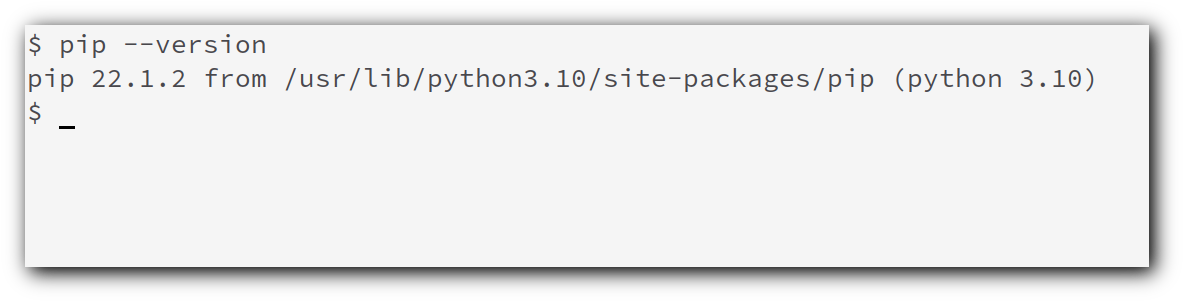
\includegraphics[width=.8\textwidth]{shots/pip-check-exists.png}
\end{center}
% }}}
% Install PIP {{{
\subsection{Install PIP}

If you do not have PIP installed, you can download and install it from this
page: \underline{\href{https://pypi.org/project/pip/}{pypi.org/project/pip}}
% }}}
% Download a Package {{{
\subsection{Download a Package}

Downloading a package is very easy.

Open the command line interface and tell PIP to download the package you want.

Navigate your command line to the location of Python's script directory, and
type the following:

\begin{center}
	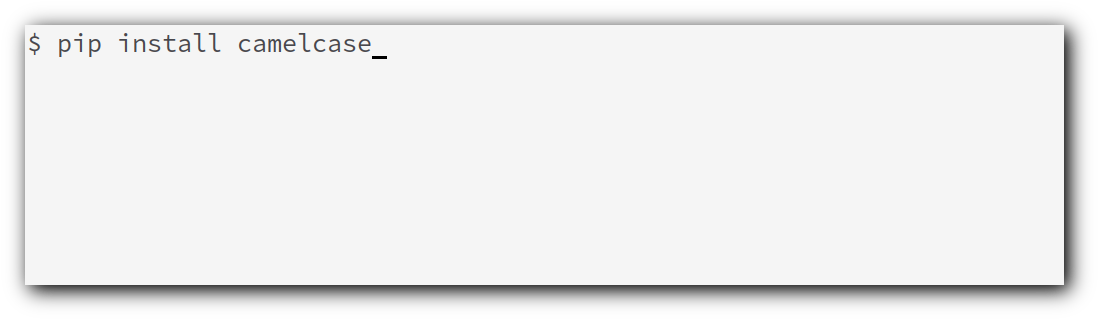
\includegraphics[width=.8\textwidth]{shots/pip-install-package.png}
\end{center}

Now you have downloaded and installed your first package!
% }}}
% Using a Package {{{
\subsection{Using a Package}

Once the package is installed, it is ready to use.

Import the ``camelcase" package into your project.

\begin{ebox}
Import and use ``camelcase":
	\begin{lstlisting}
import camelcase

c = camelcase.CamelCase()

txt = "lorem ipsum dolor sit amet"

print(c.hump(txt))

#This method capitalizes the first letter of each word.
	\end{lstlisting}
\tcblower
	\begin{vercode}
Lorem Ipsum Dolor Sit Amet
	\end{vercode}
\end{ebox}
% }}}
% Find Packages {{{
\subsection{Find Packages}

Find more packages at \underline{\href{https://pypi.org/}{pypi.org}}.
% }}}
% Remove a Package {{{
\subsection{Remove a Package}

Use the \code{uninstall} command to remove a package:

\begin{center}
	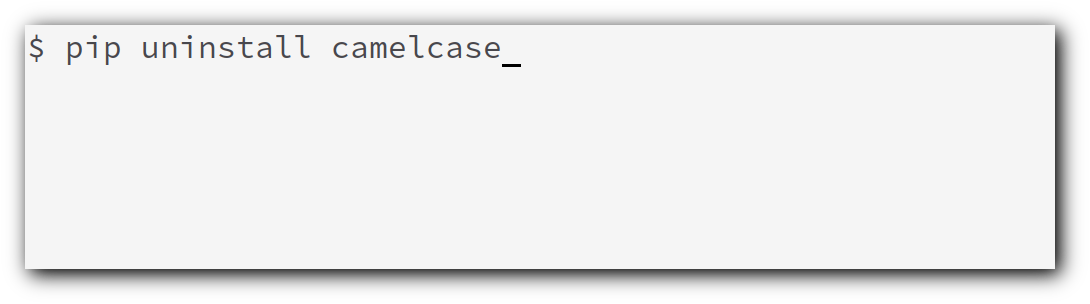
\includegraphics[width=.7\textwidth]{shots/pip-uninstall-package.png}
\end{center}

The PIP Package Manager will ask you to confirm that you want to remove the
camelcase package:

\begin{bbox}
\begin{vercode}
Uninstalling camelcase-02.1:
	Would remove:
		...
Proceed (y/n)?
\end{vercode}
\end{bbox}

Press \lcode{y} and the package will be removed.
% }}}
% List Packages {{{
\subsection{List Packages}

Use the \texttt{list} command to list all the packages installed on your system:

\begin{bbox}
	\begin{vercode}
$ pip list
Package         Version
-----------------------
camelcase       0.2
mysql-connector 2.1.6
pip             18.1
pymongo         3.6.1
setuptools      39.0.1
$_
	\end{vercode}
\end{bbox}
% }}}
% }}}
\vfill\newpage
% try...execpt {{{
\section{\textit{try ... execpt}}\label{pyTryStatement}

The \code{try} block lets you test a block of code for errors.

The \code{except} block lets you handle the error.

The \code{else} block lets you execute code when there is no error.

The \code{finally} block lets you execute code, regardless of the result of the
try and except blocks.

% Exception Handling {{{
\subsection{Exception Handling}

When an error occurs, or exception as we call it, Python will normally stop and
generate an error message.

These exceptions can be handled using the \code{try} statement:

\begin{ebox}
The \lcode{try} block will generate an exception, because x is not defined:
	\begin{lstlisting}
try:
    print(x)
except:
    print("An exception occurred")
	\end{lstlisting}
\tcblower
	\begin{vercode}
An exception occurred
	\end{vercode}
\end{ebox}

\begin{ebox}
This statement will raise an error, because \lcode{x} is not defined:
	\begin{lstlisting}
#This will raise an exception, because x is not defined:

print(x)
	\end{lstlisting}
\tcblower
	\begin{vercode}
Traceback (most recent call last):
  File "demo_try_except_error.py", line 3, in <module>
    print(x)
NameError: name 'x' is not defined
	\end{vercode}
\end{ebox}
% }}}
% Many Exceptions {{{
\subsection{Many Exceptions}

You can define as many exception blocks as you want, e.g. if you want to
execute a special block of code for a special kind of error:

\begin{ebox}
Print one message if the try block raises a \lcode{NameError} and another for other errors:
	\begin{lstlisting}
#The try block will generate a NameError, because x is not defined:

try:
    print(x)
except NameError:
    print("Variable x is not defined")
except:
    print("Something else went wrong")
	\end{lstlisting}
\tcblower
	\begin{vercode}
Variable x is not defined 
	\end{vercode}
\end{ebox}
% }}}
% Else {{{
\subsection{\textit{else}}

You can use the \code{else} keyword to define a block of code to be executed if
no errors were raised:

\begin{ebox}
In this example, the \lcode{try} block does not generate any error:
	\begin{lstlisting}
try:
    print("Hello")
except:
    print("Something went wrong")
else:
    print("Nothing went wrong")
	\end{lstlisting}
\tcblower
	\begin{vercode}
Hello
Nothing went wrong
	\end{vercode}
\end{ebox}
% }}}
% Finally {{{
\subsection{\textit{finally}}

The \code{finally} block, if specified, will be executed regardless if the try
block raises an error or not.

\begin{ebox}
	\begin{lstlisting}
try:
    print(x)
except:
    print("Something went wrong")
finally:
    print("The 'try except' is finished") 
	\end{lstlisting}
\tcblower
	\begin{vercode}
Something went wrong
The 'try except' is finished
	\end{vercode}
\end{ebox}

This can be useful to close objects and clean up resources:

\begin{ebox}
Try to open and write to a file that is not writable:
	\begin{lstlisting}
# The try block will raise an error when trying to write to a read-only file:

try:
    f = open("demofile.txt")
    try:
        f.write("Lorum Ipsum")
    except:
        print("Something went wrong when writing to the file")
    finally:
        f.close()
except:
    print("Something went wrong when opening the file")
	\end{lstlisting}
\tcblower
	\begin{vercode}
Something went wrong when writing to the file
	\end{vercode}
\end{ebox}

The program can continue, without leaving the file object open.
% }}}
% Raise an exception {{{
\subsection{\textit{raise} an \textit{exception}}

As a Python developer you can choose to throw an exception if a condition occurs.

To throw (or raise) an exception, use the \code{raise} keyword.

\begin{ebox}
Raise an error and stop the program if x is lower than 0:
	\begin{lstlisting}
x = -1

if x < 0:
    raise Exception("Sorry, no numbers below zero")
	\end{lstlisting}
\tcblower
	\begin{vercode}
Traceback (most recent call last):
  File "demo_ref_keyword_raise.py", line 4, in <module>
    raise Exception("Sorry, no numbers below zero")
Exception: Sorry, no numbers below zero
	\end{vercode}
\end{ebox}

The \code{raise} keyword is used to raise an exception.

You can define what kind of error to raise, and the text to print to the user.

\begin{ebox}
Raise a TypeError if x is not an integer:
	\begin{lstlisting}
x = "hello"

if not type(x) is int:
    raise TypeError("Only integers are allowed")
	\end{lstlisting}
\tcblower
	\begin{vercode}
Traceback (most recent call last):
  File "demo_ref_keyword_raise2.py", line 4, in <module>
    raise TypeError("Only integers are allowed")
TypeError: Only integers are allowed
	\end{vercode}
\end{ebox}
% }}}
% }}}
\vfill\newpage
% User Input {{{
\section{User \textit{input}}\label{pyUserInput}

Python allows for user input.

That means we are able to ask the user for input.

Python 3.X uses the \code{input()} method.

The following example asks for the username, and when you entered the username,
it gets printed on the screen:

\begin{ebox}
	\begin{lstlisting}
username = input("Enter username:")
print("Username is: " + username)
	\end{lstlisting}
\tcblower
	\begin{vercode}
Enter username: my user name
Username is: my user name
	\end{vercode}
\end{ebox}

\begin{nbox}
Python stops executing when it comes to the \lcode{input()} function, and
continues when the user has given some input.
\end{nbox}
% }}}
% String Formatting {{{
\section{String Formatting}\label{pyStringFormat}

To make sure a string will display as expected, we can format the result with
the \code{format()} method.

% String format() {{{
\subsection{String format()}

The \code{format()} method allows you to format selected parts of a string.

Sometimes there are parts of a text that you do not control, maybe they come
from a database, or user input?

To control such values, add placeholders (curly brackets \code{\{\}}) in the
text, and run the values through the \code{format()} method:

\begin{ebox}
Add a placeholder where you want to display the price:
	\begin{lstlisting}
price = 49
txt = "The price is {} dollars"
print(txt.format(price))
	\end{lstlisting}
\tcblower
	\begin{vercode}
The price is 49 dollars
	\end{vercode}
\end{ebox}

You can add parameters inside the curly brackets to specify how to convert the
value:

\begin{ebox}
	\begin{lstlisting}
price = 49
txt = "The price is {:.2f} dollars"
print(txt.format(price))
	\end{lstlisting}
\tcblower
	\begin{vercode}
The price is 49.00 dollars
	\end{vercode}
\end{ebox}

Check out all formatting types in \underline{String format() Reference} (Section \ref{pyRefStringFromat})
% }}}
% Multiple Values {{{
\subsection{Multiple Values}

If you want to use more values, just add more values to the format() method:

\begin{lstlisting}
print(txt.format(price, itemno, count))
\end{lstlisting}

And add more placeholders:

\begin{ebox}
	\begin{lstlisting}
quantity = 3
itemno = 567
price = 49
myorder = "I want {} pieces of item number {} for {:.2f} dollars."
print(myorder.format(quantity, itemno, price)) 
	\end{lstlisting}
\tcblower
	\begin{vercode}
I want 3 pieces of item number 567 for 49.00 dollars.
	\end{vercode}
\end{ebox}
% }}}
% Index Numbers {{{
\subsection{Index Numbers}

You can use index numbers (a number inside the curly brackets \code{\{0\}}) to be sure the values are placed in the correct placeholders:

\begin{ebox}
	\begin{lstlisting}
quantity = 3
itemno = 567
price = 49
myorder = "I want {0} pieces of item number {1} for {2:.2f} dollars."
print(myorder.format(quantity, itemno, price))
	\end{lstlisting}
\tcblower
	\begin{vercode}
I want 3 pieces of item number 567 for 49.00 dollars.
	\end{vercode}
\end{ebox}

Also, if you want to refer to the same value more than once, use the index number:

\begin{ebox}
	\begin{lstlisting}
age = 36
name = "John"
txt = "His name is {1}. {1} is {0} years old."
print(txt.format(age, name))
	\end{lstlisting}
\tcblower
	\begin{vercode}
His name is John. John is 36 years old.
	\end{vercode}
\end{ebox}
% }}}
% Named Indexes {{{
\subsection{Named Indexes}

You can also use named indexes by entering a name inside the curly brackets
\code{\{carname\}}, but then you must use names when you pass the parameter
values \code{txt.format(carname = "Ford")}:

\begin{ebox}
	\begin{lstlisting}
myorder = "I have a {carname}, it is a {model}."
print(myorder.format(carname = "Ford", model = "Mustang"))
	\end{lstlisting}
\tcblower
	\begin{vercode}
I have a Ford, it is a Mustang.
	\end{vercode}
\end{ebox}
% }}}
% }}}
%%%
% File Handling {{{
\section{File Handling}

File handling is an important part of any web application.

Python has several functions for creating, reading, updating, and deleting
files.

% Python File Open {{{
\subsection{Python File Open}

The key function for working with files in Python is the \code{open()} function.

The \code{open()} function takes two parameters; filename, and mode.

There are four different methods (modes) for opening a file:

\begin{itemize}
	\item \code{"r"} - Read - Default value. Opens a file for reading, error if the file does not exist
	\item \code{"a"} - Append - Opens a file for appending, creates the file if it does not exist
	\item \code{"w"} - Write - Opens a file for writing, creates the file if it does not exist
	\item \code{"x"} - Create - Creates the specified file, returns an error if the file exists
\end{itemize}

In addition you can specify if the file should be handled as binary or text
mode

\begin{itemize}
	\item \code{"t"} - Text - Default value. Text mode
	\item \code{"b"} - Binary - Binary mode (e.g. images)
\end{itemize}

% Syntax {{{
\subsubsection{Syntax}

To open a file for reading it is enough to specify the name of the file:

\begin{ebox}
	\begin{lstlisting}
f = open("demofile.txt")
	\end{lstlisting}
\end{ebox}

The code above is the same as:

\begin{ebox}
	\begin{lstlisting}
f = open("demofile.txt", "rt")
	\end{lstlisting}
\end{ebox}

Because \code{"r"} for read, and \code{"t"} for text are the default values,
you do not need to specify them.

% }}}
\begin{nbox}
Make sure the file exists, or else you will get an error.
\end{nbox}
% }}}
% File Read {{{
\subsection{Python File Read}

Assume we have the following file, located in the same folder as Python:

\begin{bbox}
demofile.txt:
\begin{vercode}
Hello! Welcome to demofile.txt
This file is for testing purposes.
Good Luck!
\end{vercode}
\end{bbox}

To open the file, use the built-in \code{open()} function.

The \code{open()} function returns a file object, which has a \code{read()}
method for reading the content of the file:

\begin{ebox}
	\begin{lstlisting}
f = open("demofile.txt", "r")
print(f.read())
	\end{lstlisting}
\tcblower
	\begin{vercode}
Hello! Welcome to demofile.txt
This file is for testing purposes.
Good Luck!
	\end{vercode}
\end{ebox}

If the file is located in a different location, you will have to specify the file path, like this:

\begin{ebox}
Open a file on a different location:
	\begin{lstlisting}
f = open("D:\\myfiles\welcome.txt", "r")
print(f.read())
	\end{lstlisting}
\tcblower
	\begin{vercode}
Welcome to this text file!
This file is located in a folder named "myfiles", on the D drive.
Good Luck!
	\end{vercode}
\end{ebox}

% Read Only Parts of the File {{{
\subsubsection{Read Only Parts of the File}

By default the \code{read()} method returns the whole text, but you can also
specify how many characters you want to return:

\begin{ebox}
Return the 5 first characters of the file:
	\begin{lstlisting}
f = open("demofile.txt", "r")
print(f.read(5))
	\end{lstlisting}
\tcblower
	\begin{vercode}
Hello
	\end{vercode}
\end{ebox}
% }}}
% Read Lines {{{
\subsubsection{Read Lines}

You can return one line by using the \code{readline()} method:

\begin{ebox}
Read one line of the file:
	\begin{lstlisting}
f = open("demofile.txt", "r")
print(f.readline())
	\end{lstlisting}
\tcblower
	\begin{vercode}
Hello! Welcome to demofile.txt 
	\end{vercode}
\end{ebox}

\begin{ebox}
Read two lines of the file:
	\begin{lstlisting}
f = open("demofile.txt", "r")
print(f.readline())
print(f.readline())
	\end{lstlisting}
\tcblower
	\begin{vercode}
Hello! Welcome to demofile.txt
This file is for testing purposes.
	\end{vercode}
\end{ebox}

By looping through the lines of the file, you can read the whole file, line by line:

\begin{ebox}
Loop through the file line by line:
	\begin{lstlisting}
f = open("demofile.txt", "r")
for x in f:
    print(x)
	\end{lstlisting}
\tcblower
	\begin{vercode}
Hello! Welcome to demofile.txt
This file is for testing purposes.
Good Luck!
	\end{vercode}
\end{ebox}
% }}}
% File close() Method {{{
\subsection{File close()}

It is a good practice to always close the file when you are done with it.

% Definition and Usage {{{
\subsubsection{Definition and Usage}

The \code{close()} method closes an open file.

% }}}
% Syntax {{{
\subsubsection{Syntax}

\begin{lstlisting}
file.close()
\end{lstlisting}

\begin{ebox}
Close a file after it has been opened:
	\begin{lstlisting}
f = open("demofile.txt", "r")
print(f.read())
f.close()
	\end{lstlisting}
\tcblower
	\begin{vercode}
Hello! Welcome to demofile.txt
This file is for testing purposes.
Good Luck! 
	\end{vercode}
\end{ebox}

\begin{nbox}
You should always close your files, in some cases, due to buffering, changes
made to a file may not show until you close the file.
\end{nbox}
% }}}
% }}}
% }}}
% Python File Write {{{
\subsection{Python File Write}

% Write to an Existing File {{{
\subsubsection{Write to an Existing File}

To write to an existing file, you must add a parameter to the \code{open()} function:

\begin{itemize}
	\item \code{"a"} - Append - will append to the end of the file

	\item \code{"w"} - Write - will overwrite any existing content
\end{itemize}

\begin{ebox}
Open the file ``demofile2.txt" and append content to the file:
	\begin{lstlisting}
f = open("demofile2.txt", "a")
f.write("Now the file has more content!")
f.close()

#open and read the file after the appending:
f = open("demofile2.txt", "r")
print(f.read())
	\end{lstlisting}
\tcblower
	\begin{vercode}
Hello! Welcome to demofile2.txt
This file is for testing purposes.
Good Luck!Now the file has more content! 
	\end{vercode}
\end{ebox}

\begin{ebox}
Open the file ``demofile3.txt" and overwrite the content:
	\begin{lstlisting}
f = open("demofile3.txt", "w")
f.write("Woops! I have deleted the content!")
f.close()

#open and read the file after the appending:
f = open("demofile3.txt", "r")
print(f.read())
	\end{lstlisting}
\tcblower
	\begin{vercode}
Woops! I have deleted the content!
	\end{vercode}
\end{ebox}

\begin{nbox}
	the \lcode{"w"} method will overwrite the entire file.
\end{nbox}
% }}}
% Create a New File {{{
\subsubsection{Create a New File}

To create a new file in Python, use the \code{open()} method, with one of the
following parameters:

\begin{itemize}
	\item \code{"x"} - Create - Creates the specified file, returns an error if the file exists
	\item \code{"a"} - Append - Opens a file for appending, creates the file if it does not exist
	\item \code{"w"} - Write - Opens a file for writing, creates the file if it does not exist
\end{itemize}

\begin{ebox}
Create a file called ``myfile.txt":
	\begin{lstlisting}
f = open("myfile.txt", "x")
	\end{lstlisting}
\end{ebox}

Result: a new empty file is created!

\begin{ebox}
Create a new file if it does not exist:
	\begin{lstlisting}
f = open("myfile.txt", "w")
	\end{lstlisting}
\end{ebox}
% }}}
% Delete File {{{
\subsection{Delete File}

To delete a file, you must import the OS module, and run its \code{os.remove()} function:

\begin{ebox}
Remove the file ``demofile.txt":
	\begin{lstlisting}
import os
os.remove("demofile.txt")
	\end{lstlisting}
\end{ebox}

% Check if File exist: {{{
\subsection{Check if File exist:}

To avoid getting an error, you might want to check if the file exists before
you try to delete it:

\begin{ebox}
Check if file exists, \textit{then} delete it:
	\begin{lstlisting}
import os
if os.path.exists("demofile.txt"):
    os.remove("demofile.txt")
else:
    print("The file does not exist")
	\end{lstlisting}
\end{ebox}

% }}}
% Delete Folder {{{
\subsubsection{Delete Folder}

To delete an entire folder, use the \code{os.rmdir()} method:

\begin{ebox}
Remove the folder ``myfolder":
	\begin{lstlisting}
import os
os.rmdir("myfolder")
	\end{lstlisting}
\end{ebox}

\begin{nbox}
You can only remove \textit{empty} folders.
\end{nbox}
% }}}
% }}}
% }}}
% }}}
%%%
\vfill\newpage
% Methods {{{
\section{Methods}
% String Methods {{{
\subsection{String Methods}\label{pyStringMethod}

\begin{nbox}
All string methods returns new values. They do not change the original string.
\end{nbox}

\begin{center}
	\begin{longtable}{p{.21\textwidth} p{.72\textwidth}}
	\tcol{\textbf{Method}}{\textbf{Description}}
	\tcol{\lcode{capitalize()}}
		{Converts the first character to upper case}
	\tcol{\lcode{casefold()}}
		{Converts string into lower case}
	\tcol{\lcode{center()}}
		{Returns a centered string}
	\tcol{\lcode{count()}}
		{Returns the number of times a specified value occurs in a string}
	\tcol{\lcode{encode()}}
		{Returns an encoded version of the string}
	\tcol{\lcode{endswith()}}
		{Returns true if the string ends with the specified value}
	\tcol{\lcode{expandtabs()}}
		{Sets the tab size of the string}
	\tcol{\lcode{find()}}
		{Searches the string for a specified value and returns the position of where it was found}
	\tcol{\lcode{format()}}
		{Formats specified values in a string}
	\tcol{\lcode{format_map()}}
		{Formats specified values in a string}
	\tcol{\lcode{index()}}
		{Searches the string for a specified value and returns the position of where it was found}
	\tcol{\lcode{isalnum()}}
		{Returns True if all characters in the string are alphanumeric}
	\tcol{\lcode{isalpha()}}
		{Returns True if all characters in the string are in the alphabet}
	\tcol{\lcode{isdecimal()}}
		{Returns True if all characters in the string are decimals}
	\tcol{\lcode{isdigit()}}
		{Returns True if all characters in the string are digits}
	\tcol{\lcode{isidentifier()}}
		{Returns True if the string is an identifier}
	\tcol{\lcode{islower()}}
		{Returns True if all characters in the string are lower case}
	\tcol{\lcode{isnumeric()}}
		{Returns True if all characters in the string are numeric}
	\tcol{\lcode{isprintable()}}
		{Returns True if all characters in the string are printable}
	\tcol{\lcode{isspace()}}
		{Returns True if all characters in the string are whitespaces}
	\tcol{\lcode{istitle()}}
		{Returns True if the string follows the rules of a title}
	\tcol{\lcode{isupper()}}
		{Returns True if all characters in the string are upper case}
	\tcol{\lcode{join()}}
		{Joins the elements of an iterable to the end of the string}
	\tcol{\lcode{ljust()}}
		{Returns a left justified version of the string}
	\tcol{\lcode{lower()}}
		{Converts a string into lower case}
	\tcol{\lcode{lstrip()}}
		{Returns a left trim version of the string}
	\tcol{\lcode{maketrans()}}
		{Returns a translation table to be used in translations}
	\tcol{\lcode{partition()}}
		{Returns a tuple where the string is parted into three parts}
	\tcol{\lcode{replace()}}
		{Returns a string where a specified value is replaced with a specified value}
	\tcol{\lcode{rfind()}}
		{Searches the string for a specified value and returns the last position of where it was found}
	\tcol{\lcode{rindex()}}
		{Searches the string for a specified value and returns the last position of where it was found}
	\tcol{\lcode{rjust()}}
		{Returns a right justified version of the string}
	\tcol{\lcode{rpartition()}}
		{Returns a tuple where the string is parted into three parts}
	\tcol{\lcode{rsplit()}}
		{Splits the string at the specified separator, and returns a list}
	\tcol{\lcode{rstrip()}}
		{Returns a right trim version of the string}
	\tcol{\lcode{split()}}
		{Splits the string at the specified separator, and returns a list}
	\tcol{\lcode{splitlines()}}
		{Splits the string at line breaks and returns a list}
	\tcol{\lcode{startswith()}}
		{Returns true if the string starts with the specified value}
	\tcol{\lcode{strip()}}
		{Returns a trimmed version of the string}
	\tcol{\lcode{swapcase()}}
		{Swaps cases, lower case becomes upper case and vice versa}
	\tcol{\lcode{title()}}
		{Converts the first character of each word to upper case}
	\tcol{\lcode{translate()}}
		{Returns a translated string}
	\tcol{\lcode{upper()}}
		{Converts a string into upper case}
	\tcol{\lcode{zfill()}}
		{Fills the string with a specified number of 0 values at the beginning}
	\end{longtable}
\end{center}
% }}}
%\vfill\newpage
% List Methods {{{
\subsection{List Methods}\label{pyListMethod}

\begin{table}[h]
	\begin{center}
	\begin{tabularx}{.8\textwidth}{lXl}
		\tcol{\bfseries Method}{\bfseries Description}
\tcol{\lcode{append()}}{Adds an element at the end of the list}
\tcol{\lcode{clear()}}{Removes all the elements from the list}
\tcol{\lcode{copy()}}{Returns a copy of the list}
\tcol{\lcode{count()}}{Returns the number of elements with the specified value}
\tcol{\lcode{extend()}}{Add the elements of a list (or any iterable), to the end of the current list}
\tcol{\lcode{index()}}{Returns the index of the first element with the specified value}
\tcol{\lcode{insert()}}{Adds an element at the specified position}
\tcol{\lcode{pop()}}{Removes the element at the specified position}
\tcol{\lcode{remove()}}{Removes the item with the specified value}
\tcol{\lcode{reverse()}}{Reverses the order of the list}
\tcol{\lcode{sort()}}{Sorts the list}
	\end{tabularx}
	\end{center}
\end{table}
% }}}
\vfill\newpage
% Tuple Methods {{{
\subsection{Tuple Methods}\label{pyTupleMethod}

\begin{table}[h]
	\begin{center}
		\begin{tabularx}{\textwidth}{lXl}
\tcol{\textbf{Method}}{\textbf{Description}}
\tcol{\lcode{count()}}
	{Returns the number of times a specified value occurs in a tuple}
\tcol{\lcode{index()}}
	{Searches the tuple for a specified value and returns the position of where it was found}
		\end{tabularx}
	\end{center}
\end{table}
% }}}
%\vfill\newpage
% Set Methods {{{
\subsection{Set Methods}\label{pySetMethod}

\begin{table}[h]
	\begin{center}
		\begin{tabularx}{\textwidth}{lXl}
\tcol{\textbf{Method}}{\textbf{Description}}
\tcol{\lcode{add()}}{Adds an element to the set}
\tcol{\lcode{clear()}}{Removes all the elements from the set}
\tcol{\lcode{copy()}}{Returns a copy of the set}
\tcol{\lcode{difference()}}{Returns a set containing the difference between two or more sets}
\tcol{\lcode{difference_update()}}{Removes the items in this set that are also included in another, specified set}
\tcol{\lcode{discard()}}{Remove the specified item}
\tcol{\lcode{intersection()}}{Returns a set, that is the intersection of two other sets}
\tcol{\lcode{intersection_update()}}{Removes the items in this set that are not present in other, specified set(s)}
\tcol{\lcode{isdisjoint()}}{Returns whether two sets have a intersection or not}
\tcol{\lcode{issubset()}}{Returns whether another set contains this set or not}
\tcol{\lcode{issuperset()}}{Returns whether this set contains another set or not}
\tcol{\lcode{pop()}}{Removes an element from the set}
\tcol{\lcode{remove()}}{Removes the specified element}
\tcol{\lcode{symmetric_difference()}}{Returns a set with the symmetric differences of two sets}
\tcol{\lcode{symmetric_difference_update()}}{inserts the symmetric differences from this set and another}
\tcol{\lcode{union()}}{Return a set containing the union of sets}
\tcol{\lcode{update()}}{Update the set with the union of this set and others}
		\end{tabularx}
	\end{center}
\end{table}
% }}}
\vfill\newpage
% Dictionary Methods {{{
\subsection{Dictionary Methods}\label{pyDictionaryMethod}

\begin{table}[h]
	\begin{center}
		\begin{tabularx}{\textwidth}{lXl}
\tcol{\textbf{Method}}{\textbf{Description}}
\tcol{\lcode{clear()}}{Removes all the elements from the dictionary}
\tcol{\lcode{copy()}}{Returns a copy of the dictionary}
\tcol{\lcode{fromkeys()}}{Returns a dictionary with the specified keys and value}
\tcol{\lcode{get()}}{Returns the value of the specified key}
\tcol{\lcode{items()}}{Returns a list containing a tuple for each key value pair}
\tcol{\lcode{keys()}}{Returns a list containing the dictionary's keys}
\tcol{\lcode{pop()}}{Removes the element with the specified key}
\tcol{\lcode{popitem()}}{Removes the last inserted key-value pair}
\tcol{\lcode{setdefault()}}
	{Returns the value of the specified key. If the key does not exist: insert
	the key, with the specified value}
\tcol{\lcode{update()}}{Updates the dictionary with the specified key-value pairs}
\tcol{\lcode{values()}}{Returns a list of all the values in the dictionary}
		\end{tabularx}
	\end{center}
\end{table}
% }}}
%\vfill\newpage
% Array Methods {{{
\subsection{Array Methods}\label{pyArrayMethod}

\begin{table}[h]
	\begin{center}
		\begin{tabularx}{.8\textwidth}{lXl}
			\tcol{\textbf{Method}}{\textbf{Description}}
\tcol{\lcode{append()}}{Adds an element at the end of the list}
\tcol{\lcode{clear()}}{Removes all the elements from the list}
\tcol{\lcode{copy()}}{Returns a copy of the list}
\tcol{\lcode{count()}}{Returns the number of elements with the specified value}
\tcol{\lcode{extend()}}{Add the elements of a list (or any iterable), to the end of the current list}
\tcol{\lcode{index()}}{Returns the index of the first element with the specified value}
\tcol{\lcode{insert()}}{Adds an element at the specified position}
\tcol{\lcode{pop()}}{Removes the element at the specified position}
\tcol{\lcode{remove()}}{Removes the first item with the specified value}
\tcol{\lcode{reverse()}}{Reverses the order of the list}
\tcol{\lcode{sort()}}{Sorts the list}
		\end{tabularx}
	\end{center}
\end{table}
% }}}
\vfill\newpage
% Statistics Module {{{
\subsection{\textit{statistics} Module Methods}\label{pyStatisticsModuleMethod}

Python has a built-in module that you can use to calculate mathematical
statistics of numeric data.

The \code{statistics} module was new in Python 3.4.

\begin{center}
	\begin{longtable}{p{.38\textwidth} p{.52\textwidth}}
\tcol{\textbf{Method}}{\textbf{Description}}
\tcol{\lcode{statistics.harmonic_mean()}}{Calculates the harmonic mean (central location) of the given data}
\tcol{\lcode{statistics.mean()}}{Calculates the mean (average) of the given data}
\tcol{\lcode{statistics.median()}}{Calculates the median (middle value) of the given data}
\tcol{\lcode{statistics.median_grouped()}}{Calculates the median of grouped continuous data}
\tcol{\lcode{statistics.median_high()}}{Calculates the high median of the given data}
\tcol{\lcode{statistics.median_low()}}{Calculates the low median of the given data}
\tcol{\lcode{statistics.mode()}}{Calculates the mode (central tendency) of the given numeric or nominal data}
\tcol{\lcode{statistics.pstdev()}}{Calculates the standard deviation from an entire population}
\tcol{\lcode{statistics.stdev()}}{Calculates the standard deviation from a sample of data}
\tcol{\lcode{statistics.pvariance()}}{Calculates the variance of an entire population}
\tcol{\lcode{statistics.variance()}}{Calculates the variance from a sample of data}
	\end{longtable}
\end{center}
% }}}
%\vfill\newpage
% Math Module {{{
\subsection{\textit{math} Module}\label{pyMathModuleMethod}

\begin{center}
	\begin{longtable}{p{.18\textwidth} p{.72\textwidth}}
\tcol{\textbf{Method}}{\textbf{Description}}
\tcol{\lcode{acos()}}{Returns the arc cosine of a number}
\tcol{\lcode{acosh()}}{Returns the inverse hyperbolic cosine of a number}
\tcol{\lcode{asin()}}{Returns the arc sine of a number}
\tcol{\lcode{asinh()}}{Returns the inverse hyperbolic sine of a number}
\tcol{\lcode{atan()}}{Returns the arc tangent of a number in radians}
\tcol{\lcode{atan2()}}{Returns the arc tangent of y/x in radians}
\tcol{\lcode{atanh()}}{Returns the inverse hyperbolic tangent of a number}
\tcol{\lcode{ceil()}}{Rounds a number up to the nearest integer}
\tcol{\lcode{comb()}}{Returns the number of ways to choose k items from n items
		without repetition and order}
\tcol{\lcode{copysign()}}{Returns a float consisting of the value of the first
		parameter and the sign of the second parameter}
\tcol{\lcode{cos()}}{Returns the cosine of a number}
\tcol{\lcode{cosh()}}{Returns the hyperbolic cosine of a number}
\tcol{\lcode{degrees()}}{Converts an angle from radians to degrees}
\tcol{\lcode{dist()}}{Returns the Euclidean distance between two points (p and
		q), where p and q are the coordinates of that point}
\tcol{\lcode{erf()}}{Returns the error function of a number}
\tcol{\lcode{erfc()}}{Returns the complementary error function of a number}
\tcol{\lcode{exp()}}{Returns E raised to the power of x}
\tcol{\lcode{expm1()}}{Returns Ex - 1}
\tcol{\lcode{fabs()}}{Returns the absolute value of a number}
\tcol{\lcode{factorial()}}{Returns the factorial of a number}
\tcol{\lcode{floor()}}{Rounds a number down to the nearest integer}
\tcol{\lcode{fmod()}}{Returns the remainder of x/y}
\tcol{\lcode{frexp()}}{Returns the mantissa and the exponent, of a specified number}
\tcol{\lcode{fsum()}}{Returns the sum of all items in any iterable (tuples,
		arrays, lists, etc.)}
\tcol{\lcode{gamma()}}{Returns the gamma function at x}
\tcol{\lcode{gcd()}}{Returns the greatest common divisor of two integers}
\tcol{\lcode{hypot()}}{Returns the Euclidean norm}
\tcol{\lcode{isclose()}}{Checks whether two values are close to each other, or not}
\tcol{\lcode{isfinite()}}{Checks whether a number is finite or not}
\tcol{\lcode{isinf()}}{Checks whether a number is infinite or not}
\tcol{\lcode{isnan()}}{Checks whether a value is NaN (not a number) or not}
\tcol{\lcode{isqrt()}}{Rounds a square root number downwards to the nearest integer}
\tcol{\lcode{ldexp()}}{Returns the inverse of math.frexp() which is x * (2**i)
		of the given numbers x and i}
\tcol{\lcode{lgamma()}}{Returns the log gamma value of x}
\tcol{\lcode{log()}}{Returns the natural logarithm of a number, or the
		logarithm of number to base}
\tcol{\lcode{log10()}}{Returns the base-10 logarithm of x}
\tcol{\lcode{log1p()}}{Returns the natural logarithm of 1+x}
\tcol{\lcode{log2()}}{Returns the base-2 logarithm of x}
\tcol{\lcode{perm()}}{Returns the number of ways to choose k items from n items
		with order and without repetition}
\tcol{\lcode{pow()}}{Returns the value of x to the power of y}
\tcol{\lcode{prod()}}{Returns the product of all the elements in an iterable}
\tcol{\lcode{radians()}}{Converts a degree value into radians}
\tcol{\lcode{remainder()}}{Returns the closest value that can make numerator
		completely divisible by the denominator}
\tcol{\lcode{sin()}}{Returns the sine of a number}
\tcol{\lcode{sinh()}}{Returns the hyperbolic sine of a number}
\tcol{\lcode{sqrt()}}{Returns the square root of a number}
\tcol{\lcode{tan()}}{Returns the tangent of a number}
\tcol{\lcode{tanh()}}{Returns the hyperbolic tangent of a number}
\tcol{\lcode{trunc()}}{Returns the truncated integer parts of a number}
	\end{longtable}
\end{center}

\subsubsection{Math Constants}

\begin{center}
	\begin{longtable}{p{.25\textwidth} p{.65\textwidth}}
\tcol{\textbf{Constant}}{\textbf{Description}}
\tcol{\lcode{math.e}}{Returns Euler's number (2.7182...)}
\tcol{\lcode{math.inf}}{Returns a floating-point positive infinity}
\tcol{\lcode{math.nan}}{Returns a floating-point NaN (Not a Number) value}
\tcol{\lcode{math.pi}}{Returns PI (3.1415...)}
\tcol{\lcode{math.tau}}{Returns tau (6.2831...)}
	\end{longtable}
\end{center}
% }}}
%\vfill\newpage
% Random Module {{{
\subsection{\textit{random} Module}\label{pyRandomModuleMethod}

\begin{center}
	\begin{longtable}{p{.28\textwidth} p{.65\textwidth}}
\tcol{\textbf{Method}}{\textbf{Description}}
\tcol{\lcode{seed()}}{Initialize the random number generator}
\tcol{\lcode{getstate()}}{Returns the current internal state of the random number generator}
\tcol{\lcode{setstate()}}{Restores the internal state of the random number generator}
\tcol{\lcode{getrandbits()}}{Returns a number representing the random bits}
\tcol{\lcode{randrange()}}{Returns a random number between the given range}
\tcol{\lcode{randint()}}{Returns a random number between the given range}
\tcol{\lcode{choice()}}{Returns a random element from the given sequence}
\tcol{\lcode{choices()}}{Returns a list with a random selection from the given sequence}
\tcol{\lcode{shuffle()}}{Takes a sequence and returns the sequence in a random order}
\tcol{\lcode{sample()}}{Returns a given sample of a sequence}
\tcol{\lcode{random()}}{Returns a random float number between 0 and 1}
\tcol{\lcode{uniform()}}{Returns a random float number between two given parameters}
\tcol{\lcode{triangular()}}{Returns a random float number between two given
		parameters, you can also set a mode parameter to specify the midpoint
		between the two other parameters}
\tcol{\lcode{betavariate()}}{Returns a random float number between 0 and 1
		based on the Beta distribution (used in statistics)}
\tcol{\lcode{expovariate()}}{Returns a random float number based on the
		Exponential distribution (used in statistics)}
\tcol{\lcode{gammavariate()}}{Returns a random float number based on the Gamma
		distribution (used in statistics)}
\tcol{\lcode{gauss()}}{Returns a random float number based on the Gaussian
		distribution (used in probability theories)}
\tcol{\lcode{lognormvariate()}}{Returns a random float number based on a
		log-normal distribution (used in probability theories)}
\tcol{\lcode{normalvariate()}}{Returns a random float number based on the
		normal distribution (used in probability theories)}
\tcol{\lcode{vonmisesvariate()}}{Returns a random float number based on the von
		Mises distribution (used in directional statistics)}
\tcol{\lcode{paretovariate()}}{Returns a random float number based on the
		Pareto distribution (used in probability theories)}
\tcol{\lcode{weibullvariate()}}{Returns a random float number based on the
		Weibull distribution (used in statistics)}
	\end{longtable}
\end{center}
% }}}
%\vfill\newpage
% Requests Module {{{
\subsection{\textit{requests} Module Methods}\label{pyRequestsModuleMethod}

\begin{ebox}
Make a request to a web page, and print the response text:
	\begin{lstlisting}
import requests

x = requests.get('https://w3schools.com/python/demopage.htm')

print(x.text)
	\end{lstlisting}
\tcblower
	\begin{vercode}
<!DOCTYPE html>
<html>
<body>

<h1>This is a Test Page</h1>

</body>
</html> 
	\end{vercode}
\end{ebox}
% Definition and Usage {{{

\subsubsection{Definition and Usage}

The \code{requests} module allows you to send HTTP requests using Python.

The HTTP request returns a Response Object with all the response data (content,
encoding, status, etc).
% }}}
% Download and Install the Requests Module {{{
\subsubsection{Download and Install the Requests Module}

Navigate your command line to the location of PIP, and type the following:

\begin{bbox}
	\begin{vercode}
$ pip install requests
	\end{vercode}
\end{bbox}
% }}}
% Syntax {{{
\subsubsection{Syntax}

\begin{bbox}
	\begin{vercode}
requests.methodname(params)
	\end{vercode}
\end{bbox}
% }}}
% Methods {{{
\subsubsection{Methods}

\begin{center}
	\begin{longtable}{p{.389\textwidth} p{.52\textwidth}}
\tcol{\textbf{Method}}{\textbf{Description}}
\tcol{\lcode{delete(url, args)}}{Sends a DELETE request to the specified url}
\tcol{\lcode{get(url, params, args)}}{Sends a GET request to the specified url}
\tcol{\lcode{head(url, args)}}{Sends a HEAD request to the specified url}
\tcol{\lcode{patch(url, data, args)}}{Sends a PATCH request to the specified url}
\tcol{\lcode{post(url, data, json, args)}}{Sends a POST request to the specified url}
\tcol{\lcode{put(url, data, args)}}{Sends a PUT request to the specified url}
\tcol{\lcode{request(method, url, args)}}{Sends a request of the specified method to the specified url}
	\end{longtable}
\end{center}

% }}}
% }}}
%\vfill\newpage
% }}}

% }}}
% }}}
\end{document}
